\newcommand{\microns}{$\upmu$m\xspace}
\newcommand{\etal}{\textit{et al.}\xspace}
\newcommand{\Ef}{$E_{F}$\xspace}
\newcommand{\SiO}{SiO$_{2}$\xspace}
\newcommand{\insitu}{\textit{in situ}\xspace}
\newcommand{\Ohms}{$\Omega$\xspace}


\newcommand{\InsertFig}[3]{
  \begin{figure}[!htbp]
    \begin{center}
      \leavevmode
      #1
      \caption{#2}
      \label{#3}
    \end{center}
  \end{figure}
}




\documentclass[oneside,11pt]{Classes/myThesis}
%%%%%%%%%%%%%%%%%%%%%%%%%%%%%%%%%%%%%%%%%%%%%%%%%%%%%%
%%%%%%%%%%%%%%% file path for figures - add extra chapters as necessary %%%%%%%%%
%%%%%%%%%%%%%%%%%%%%%%%%%%%%%%%%%%%%%%%%%%%%%%%%%%%%%%
\graphicspath{{./Chapters/Chapter_1_Introduction}     
              {./Chapters/Chapter_2_Background}
              {./Chapters/Chapter_3_Numerical_Simulation}
              {./Chapters/Chapter_4_Parameter_Space_Paper}
              {./Chapters/Chapter_5_Real_Systems_Paper}
              {./Chapters/Chapter_6_Terminal_Velocity_Paper}
              {./Chapters/Chapter_7_Final_Notes}
              {./ThesisFigs/}}

%%%%%%%%%%%%%%%%%%%%%%%%%%%%%%%%%%%%%%%%%%%%%%%%%%%%%%
%%%%%%%%%%%%% Constants - fill these in for use throughout the thesis %%%%%%%%%%%%
%%%%%%%%%%%%%%%%%%%%%%%%%%%%%%%%%%%%%%%%%%%%%%%%%%%%%%
\newcommand{\theAuthor}{Joseph Eatson}
\newcommand{\authorEmail}{py13je@leeds.ac.uk}
\newcommand{\myTitle}{Numerical Simulations of Dusty Colliding Wind Binaries}

%%%%%%%%%%%%%%%%%%%%%%%%%%%%%%%%%%%%%%%%%%%%%%%%%%%%%%
\pdfinfo { /Title  (\myTitle)
           /Creator (TeX)
           /Producer (pdfTeX)
           /Author (\theAuthor \authorEmail)
           /ModDate (D:\pdfdate)
           /CreationDate (D:\pdfdate)  %format D:YYYYMMDDhhmmss
           /Subject (Astrophysics)
           /Keywords (PhD, Thesis)}    
		\pdfcatalog { /PageMode (/UseOutlines)
                  /OpenAction (fitbh)  }

%%%%%%%%%%%%%%%%%%%%%%%%%%%%%%%%%%%%%%%%%%%%%%%%%%%%%%
%%%%%%%%%%%%% Title Page Information %%%%%%%%%%%%%%%%%%%%%%%%%%%%
%%%%%%%%%%%%%%%%%%%%%%%%%%%%%%%%%%%%%%%%%%%%%%%%%%%%%%
\title{\myTitle}
\author{\href{mailto:\authorEmail}{\theAuthor}}
\crest{
\includegraphics[width=35mm]{Leeds_Crest.eps}}
%%%%%%%%%%%%%%%%%%%%%%%%%%%%%%%%%%%%%%%%%%%%%%%%%%%%%%
%% Define these as empty to omit the two logos on the title page
%%%%%%%%%%%%%%%%%%%%%%%%%%%%%%%%%%%%%%%%%%%%%%%%%%%%%%
\logo{
\includegraphics[width=50mm]{Leeds.pdf}} %University Logo
\deptlogo{} %\includegraphics[width=50mm]{UoL_logo}} % Institute Logo
%%%%%%%%%%%%%%%%%%%%%%%%%%%%%%%%%%%%%%%%%%%%%%%%%%%%%%
\collegeordept{\href{http://physics.leeds.ac.uk}{School of Physics and Astronomy}}
\university{\href{http://www.leeds.ac.uk}{University of Leeds}}

\degree{Doctor of Philosophy}
\degreedate{\monthdate\today}

%Different font in captions
%Different font in caption
%%%%%%%%%%%%%%%%%%%%%%%%%%%%%%%%%%%%%%%%%%%%%%%%%%%%%%
%%%%%%%%%%%%%%%% Optional Packages  %%%%%%%%%%%%%%%%%%%%%%%%%%%
%%%%%%%%%%%%%%%%%%%%%%%%%%%%%%%%%%%%%%%%%%%%%%%%%%%%%%
%\usepackage{StyleFiles/watermark}
%\usepackage{xspace}  %add a space after maths if not already there
%\usepackage{booktabs} %better tables
%\usepackage{rotating}  %rotating figures and tables
%\usepackage{array} %enhanced tables
%\usepackage{ctable} %include a figure command
%\usepackage{footnote}
%\usepackage{multirow} %for merging cells on tables
%\usepackage{times} % The "Times" font
%\usepackage{Utopia} % The "Utopia" font

\usepackage{siunitx} % Better units, especially SI
\sisetup{separate-uncertainty=true,   % Allow uncertainties
         print-unity-mantissa=false,  % If 1e2, write as 10^2 not 1x10^2
         group-minimum-digits=4,      % Start separating > 999, not > 9,999
         group-separator = {,}}       % Unit now 1,000 instead of 1000

\usepackage{mathtools}
% Better tables
\usepackage{longtable}
\usepackage{booktabs}
\usepackage{floatrow}
\DeclareFloatFont{scriptsize}{\scriptsize}
\floatsetup[table]{font=scriptsize}
%Captions for subfigures
% \usepackage[format=hang,labelfont=bf]{caption}
\usepackage[format=hang,labelfont={bf,scriptsize},font=scriptsize]{caption}

\usepackage{tikz}
\usetikzlibrary{shapes.geometric, arrows}
\usepackage{spreadtab}

% Hyphen texttt{}
\usepackage[htt]{hyphenat}

% Define block styles
\tikzstyle{decision} = [diamond, draw, fill=blue!20, 
    text width=8em, text badly centered, inner sep=0pt]
\tikzstyle{block} = [rectangle, draw, fill=blue!20, 
    text width=8em, text centered, rounded corners, minimum height=4em]
\tikzstyle{line} = [draw, -latex']
\tikzstyle{cloud} = [draw, ellipse,fill=red!20, node distance=3cm, text width=5em, minimum height=2em]

\usepackage{listings}
\usepackage{xcolor}
\usepackage[super]{nth} % Allows for superscripting numbers

% Colour style for programming markup, using nord scheme https://www.nordtheme.com/
\definecolor{codetext}{HTML}{2e3440}
\definecolor{codegreen}{HTML}{a3be8c}
\definecolor{codegray}{HTML}{d8dee9}
\definecolor{codeblue}{HTML}{5e81ac}
\definecolor{codeorange}{HTML}{d08770}
\definecolor{backcolour}{HTML}{eceff4}
\lstdefinestyle{nord}{
    backgroundcolor=\color{backcolour},
    commentstyle=\color{codegreen},
    keywordstyle=\color{codeorange},
    numberstyle=\ttfamily\footnotesize\color{codegray},
    stringstyle=\color{codeblue},
    basicstyle=\ttfamily\footnotesize\color{codetext},
    breakatwhitespace=false,
    breaklines=true,
    captionpos=b,
    keepspaces=true,
    numbers=left,
    numbersep=5pt,
    showspaces=false,
    showstringspaces=false,
    showtabs=false,
    tabsize=2
}
\lstset{style=nord}

% Text macros
\newcommand{\tx}{\text}
\newcommand{\ts}{\textsuperscript}
\newcommand{\mg}{\texttt{MG}}
\newcommand{\athena}{\texttt{Athena++}}
\newcommand{\link}[1]{\texttt{\href{#1}{#1}}}
\newcommand{\footlink}[2]{\href{#2}{#1}\footnote{\texttt{\href{#2}{#2}}}}

% Math macros 
\newcommand{\swr}{\ensuremath{_{\text{WR}}}}
\newcommand{\sob}{\ensuremath{_{\text{OB}}}}
\newcommand{\rms}[1]{\ensuremath{_\text{#1}}}
\newcommand{\mdot}{\ensuremath{\dot{\text{M}}}}
\newcommand{\mass}{\ensuremath{\text{M}}}
\newcommand{\lumin}{\ensuremath{\text{L}}}
\newcommand{\vinf}{\ensuremath{v^\infty}}
\newcommand{\dsep}{d\rms{sep}}

\newcommand{\sol}{\ensuremath{_{\odot}}}

\newcommand{\atom}[3]{\prescript{#2}{#3}{\text{#1}}}

% Setup for BibLaTeX, used instead of BibTeX as it is more flexible
\usepackage[
  style=apa,        % Use American Psychological Association style
  backref=true,     % Link back to citation pages in bibliography
  backend=biber,    % Use biber to process citations
  bibencoding=utf8, % Ensure UTF8 encoding for fancy characters
  url=false,        % Don't show URLs
  doi=true,        % Don't show DOIs
  isbn=true        % Don't show ISB numbers
]{biblatex}
% Point biber towards bibliography
\addbibresource{References/library-biblatex.bib} 
% Sylistic changes to bibliography 
\DefineBibliographyStrings{english}{
  backrefpage = {cit. p.},     % originally "cited on page"
  backrefpages = {cit. p.},   % originally "cited on pages"
}
\DeclareFieldFormat{doi}{\\ \footnotesize{DOI: \texttt{\href{https://doi.org/#1}{#1}}}}
% \DeclareFieldFormat{url}{\\ \footnotesize{URL: \texttt{\url{#1}}}}

% Ensure addendums are not shown
\AtEveryBibitem{\clearfield{note}\clearfield{addendum}\clearfield{annotation}} 
\AtEveryCitekey{\clearfield{note}\clearfield{addendum}\clearfield{annotation}}
% Ensure annotations are not shown
\AtEveryBibitem{\clearfield{note}}
\AtEveryCitekey{\clearfield{note}\clearfield{annotation}}

\linespread{1.3} %1.5 line spacing

%%%%%%%%%%%%%%%%%%%%%%%%%%%%%%%%%%%%%%%%%%%%%%%%%%%%%%
%%%%% Uncommon units %%%%%%%%%%%%%%%%%%%%%%%%%%%%%%%%%

\DeclareSIUnit[]\solarmass
{\text{\ensuremath{\textup{M}_{\odot}}}}
\DeclareSIUnit[]\solarluminosity
{\text{\ensuremath{\textup{L}_{\odot}}}}
\DeclareSIUnit[]\solarradius
{\text{\ensuremath{\textup{R}_{\odot}}}}
\DeclareSIUnit[]\year
{\text{yr}}
\DeclareSIUnit[]\au
{\text{AU}}
\DeclareSIUnit[]\parsec
{\text{pc}}
\DeclareSIUnit[]\erg
{\text{erg}}
\DeclareSIUnit[]\arcsecond
{\text{as}}
\DeclareSIUnit[]\angstrom{\textup{\AA}}

\newlength\longest

\begin{document}
%\baselineskip=18pt plus1pt

\maketitle
%set the number of sectioning levels that get number and appear in the contents
\setcounter{secnumdepth}{2}
\setcounter{tocdepth}{2}
\pagenumbering{roman}
\frontmatter
%%%%%%%%%%%%%%%%%%%%%%%%%%%%%%%%%%%%%%%%%%%%%%%%%%%%%%
%%%%%%%%%%%% Include sections are required, or comment out to skip over %%%%%%%%%
%%%%%%%%%%%%%%%%%%%%%%%%%%%%%%%%%%%%%%%%%%%%%%%%%%%%%%
% Thesis Dedictation ---------------------------------------------------

\begin{dedication} %this creates the heading for the dedication page

To my Mum, without her help these past 27 years there's no way I would have gotten this far.

Thank you so much, for everything.

\end{dedication}

% ----------------------------------------------------------------------

%%% Local Variables: 
%%% mode: latex
%%% TeX-master: "../thesis"
%%% End: 

% % Thesis IP Statement ---------------------------------------------------

\begin{ipstatement} %this creates the heading for the dedication page

I am aware that the University defines plagiarism as presenting someone else’s work, in whole or in part, as your own. Work means any intellectual output, and typically includes text, data, images, sound or performance.

I promise that in the attached submission I have not presented anyone else’s work, in whole or in part, as my own and I have not colluded with others in the preparation of this work. Where I have taken advantage of the work of others, I have given full acknowledgement.I have not resubmitted my own work or part thereof without specific written permission to do so from the University staff concerned when any of this work has been or is being submitted for marks or credits even if in a different module or for a different qualification or completed prior to entry to the University. I have read and understood the University’s published rules on plagiarism and also any more detailed rules specified at School or module level.I know that if I commit plagiarism I can be expelled from the University and that it is my responsibility to be aware of the University’s regulations on plagiarism and their importance.

I re-confirm my consent to the University copying and distributing any or all of my work in any form and using third parties (who may be based outside the EU/EEA) to monitor breaches of regulations, to verify whether my work contains plagiarised material, and for quality assurance purposes. 

I confirm that I have declared all mitigating circumstances that may be relevant to the assessment of this piece of work and that I wish to have taken into account.I am aware of the University’s policy on mitigation and the School’s procedures for the submission of statements and evidence of mitigation. I am aware of the penalties imposed for the late submission of coursework.
\\
\vspace{1cm}

{\large Signed :\space}\rule{7cm}{0.2pt}{\large \space Date}\hrulefill\\

\hspace*{1.5cm}\theAuthor

\vspace{1cm}

\copyright \yeardate\today The University of Leeds and \theAuthor.

\end{ipstatement}

% ----------------------------------------------------------------------

%%% Local Variables: 
%%% mode: latex
%%% TeX-master: "../thesis"
%%% End: 


\clearpage

% \pagestyle{plain}
% \null\vfill
% \begin{center}
%   \parbox{0.5\textwidth}{%
%     \raggedright{\large\itshape%
%     ``Space is \textbf{big}. Really big. You just won't believe how vastly, hugely, mind-bogglingly big it is. I mean, you may think it's a long way down the road to the chemist's, but that's just peanuts to space.''
%     \par%\bigskip
%     }
%     \rule{\linewidth}{0.4pt}
%     \raggedleft{\Large\MakeUppercase{Douglas Adams}\\\large\itshape{The Hitchhiker's Guide to the Galaxy}\par}%
%   }
% \end{center}
% \vfill\vfill

\begin{dedication}
  \begin{center}
    \parbox{0.5\textwidth}{
      \raggedright{
        \emph{
          ``Space is \textbf{big}. Really big. You just won't believe how vastly, hugely, mind-bogglingly big it is. I mean, you may think it's a long way down the road to the chemist's, but that's just peanuts to space.''
        }
        \par
      }
      \raggedleft{
        \rule{\linewidth}{0.5pt}
        \Large
        \MakeUppercase{Douglas Adams}
        \\
        \large
        \emph{The Hitchhiker's Guide to the Galaxy}
        \par
      }
    }
    \vfill
  \end{center}
\end{dedication}

\begin{dedication}
  \begin{center}
    \parbox{0.5\textwidth}{
      \vspace{1em}
      \raggedright{
        \emph{
          ``I am aware that quoting Douglas Adams in an astrophysics thesis is an absolutely enormous clich\'{e}, but I want to do it anyway.''
        }
        \par
      }
      \raggedleft{
        \rule{\linewidth}{0.5pt}
        \Large
        \MakeUppercase{Me}
        \\
        \large
        \emph{This Thesis}
        \par
      }
    }
  \end{center}
  \vfill
\end{dedication}

\clearpage

% Thesis Acknowledgements ------------------------------------------------


%\begin{acknowledgementslong} %uncommenting this line, gives a different acknowledgements heading
\begin{acknowledgements}      %this creates the heading for the acknowlegments

\setlength{\parindent}{17.62482pt}
\setlength{\parskip}{0.0pt plus 1.0pt}

\textbf{If you're reading this ahead of time and wondering where you are, don't worry, I'm getting to you, just writing the thesis first!}

I suppose a good place to start when thanking people in a thesis is to start with family.
To my mum, when I asked you to for help funding my doctoral degree, you said yes, instantly, and without hesitation, considering all you have done and sacrificed for me throughout my life, your agreeing to help was another act of kindness that I can barely repay (trust me, I've done the maths).
You've been there for me, every step of the way, I could not ask for a more wonderful mum, and I hope I can make you proud.

I also owe a debt to my supervisor, Dr. Julian Pittard, you've gone above and beyond when it came to my supervision, you've solved bugs, found mistakes and gotten me out of a jam more times in this project than I can count.
I'm still amazed how you can rattle off a paper or three from memory when I've come into your office asking questions about a very specific part of my work.
Honestly, how do you do that? It's very impressive.

No good thesis\footnote{Though the quality of this one is debatable.} wouldn't be complete without a commitment to the authors friends.
I first met some of you on the literal first day of my undergraduate degree, it's really quite incredible how you've all tolerated my nonsense for so long.
From essentially forcing my way into Rob's house so I could cook some disastrous fried chicken, to playing \textit{Super Smash Bros.} all night long on it's release day, to watching trashy movies over the internet at the height of a global pandemic, these are moments I'll treasure for the rest of my life.
In particular, those who are still in Leeds, Rob\footnote{\emph{``People can put whatever they want in footnotes, nobody reads them.''} - Dr. Rob Welch}, Matt, Kelsie, Alex and Sam; as well as those who aren't, Martin, Caz, Andy, and Devon.
Thank you all, for filling my life with joy this past decade.
To my partner Pruthvi, I cannot stress how unlikely it is that the two of us even met - two people finding and falling for each other on the more esoteric circles of the internet is like two particles colliding in the tenuous interstellar medium, if you'll excuse the extremely trite metaphor.
You've been loving, kind, helpful, and the most wonderful partner anyone could ask for.
I truly am blessed to know you and love you.

I would also like to thank the fantastic team at Leeds' ARC High Performance Computing department, considering the bulk of this work involves many 3D numerical simulations my use of ARC 4's compute nodes can be described as somewhere from ``excessive'' to ``taking the piss''.
I also apologise for running my earlier simulations on the login nodes for multiple days, I swear it was an accident.

I would also like to thank two figures from my formative years for inspiring me.
The first is my 9\textsuperscript{th} year Physics teacher, Isobel Why, who re-kindled my interest in the field, she was the finest teacher I ever had, turning me from an underachieving student to a keen and committed aspiring physicist.
She truly had faith in all of her students, and pushed them far beyond what they thought themselves capable of.
Whilst she left teaching shortly after that year, I will never forget her impact on my life and my work.
Another is quite indirect, but still important, I would be amiss to thank Winchell ``Nyrath'' Chung, curator of the website \footlink{Atomic Rockets}{http://projectrho.com/public\_html/rocket/}.
Winchell's work is perhaps one of the most complete and exhaustive archive of real life and fictional rocketry and space exploration resources - whilst I haven't called on his work much during my career in astrophysics, I pored over this website when I was younger (perhaps reading it more thoroughly than any of my course textbooks).
It was fascinating, insightful and inspiring not only to me, but thousands of readers; the number of projects, from hard SFF novellas to honest-to-goodness research proposals hinge on his tireless efforts to catalogue humankind's exploration of space in both reality and fiction.
I learned of his cancer diagnosis whilst writing this thesis, and it cut me to my core, without his work I don't think I would have turned a fascination with space into a lifelong passion.
Thank you so much, both of you, you may not realise it, you may not ever read this, but you changed my life.

% This one might need to be moved, considering the above paragraph 
Finally, I would like to thank Leandro Panizzon and his wife, Margarita, though Methylphenidate was originally synthesised by him to treat her low blood pressure, it also works quite well for dragging my attention-deficit disorder riddled brain through this PhD.

\end{acknowledgements}
%\end{acknowledgmentslong}

% ------------------------------------------------------------------------

%%% Local Variables: 
%%% mode: latex
%%% TeX-master: "../thesis"
%%% End: 


% Thesis Abstract -----------------------------------------------------


%\begin{abstractslong}    %uncommenting this line, gives a different abstract heading
\begin{abstracts}        %this creates the heading for the abstract page

\setlength{\parindent}{17.62482pt}
\setlength{\parskip}{0.0pt plus 1.0pt}

\note{Colliding Wind Binary (CWB) systems are relatively rare phenomena, but have a significant influence on galactic evolution in terms of dust production -- especially in the early universe.
The mechanisms behind this dust production, however, are poorly understood.
The strong winds from both partners in the binary system drive shocks that heat the dust forming region to temperatures in excess of \SI{1e8}{K}; whilst this region does rapidly cool, the initial shock temperatures would destroy any dust grains that formed outside the collision region.
Furthermore, this collision region is difficult to observe and simulate, limiting our understanding of how grains form and evolve in this region.}

\note{This thesis attempts to improve our understanding of the evolution of dust grains within these systems, particularly growth of these grains from small dust grain cores to micron-scale grains.
A co-moving dust grain model was implemented that simulates growth through accretion of gas onto the dust grains, as well as destruction through gas-grain sputtering.
The model also simulates cooling through collisional excitation and subsequent emission for both dust grains and gas.
Overall, the goal of this model was to determine how dust growth was influenced by the wind and orbital characteristics of the system, and which of these characteristics were most important for dust growth.}

\note{First, a parameter space exploration of dust producing CWB systems (WCd systems) was conducted, varying the orbital separation ($\dsep$), the wind terminal velocity ($\vinf$) and the mass loss rate ($\mdot$) of each star.
It was found that dust production is strongly influenced by the ratio of wind terminal velocities between each star, as well as the orbital separation.
Following up on this, a limited simulation of the episodic dust forming system WR140 was conducted, in order to understand how variance in orbital separation through eccentricity changed dust production rates over the course of a periastron passage.
Furthermore, it was determined that dust production occurs over a very short period immediately prior to periastron passage and a small period after, with an ``active'' phase of approximately 1 year, or $1/8$\textsuperscript{th} of the systems orbital period}

\note{Whilst there is much to be done in the future, and many more systems to be simulated (in particular the recently discovered WR+WR CWB systems WR48a and WR70-16) this model is a good first step towards shedding light on these elusive and dust-shrouded systems.}

\end{abstracts}
%\end{abstractlongs}

% ----------------------------------------------------------------------

%%% Local Variables: 
%%% mode: latex
%%% TeX-master: "../thesis"
%%% End: 

\newpage
\tableofcontents
\newpage
\listoffigures
\newpage
\listoftables
\newpage

\begin{abbreviations}
List of common abbreviations, if an abbreviation is important enough to warrant a section in this thesis, the section will be referenced.

\begin{table}[h]
  \centering
  \begin{tabular}{l|l|l}
    
    \hline

    3$\alpha$ & Triple-$\alpha$ helium burning & \ref{sec:evolvedstars} \\
    AGB & Asymptotic Giant Branch & \ref{sec:evolvedstars} \\
    BODMAS & Binary Orbit Dust Model with Accretion and Sputtering & Section \ref{sec:bodmas} \\
    CAK & Castor, Abbott \& Klein (\citeyear{castor_radiation-driven_1975}) theory \& Section \ref{sec:cak} \\
    CWB & Colliding Wind Binary  & Section \ref{sec:obtype} \\
    FGC & Fighting Game Community & Section \ref{sec:wcrcooling} \\
    GCR & Galactic Cosmic Ray & Section \ref{sec:wcrcooling} \\
    GMC & Giant Molecular Cloud & Section \ref{sec:obtype}\\
    ISM & Interstellar Medium & Section \ref{sec:earlytype} \\
    KH  & Kelvin-Helmholtz & \ref{sec:earlytype} \\ 
    LBV & Luminous Blue Variable & Section \ref{sec:obtype} \\
    OB  & O or B type star & Section \ref{sec:obtype} \\ 
    RSG & Red Supergiant & Section \ref{sec:obtype} \\
    WC  & WR Carbon Phase & Section \ref{sec:wrtype} \\
    WCd & Dust forming WC star & Section \ref{sec:cwbdust} \\
    WCR & Wind Collision Region & Section \ref{sec:wcr} \\
    WN  & WR Nitrogen Phase & Section \ref{sec:wrtype} \\
    WO  & WR Oxygen Phase & Section \ref{sec:wrtype} \\
    WR  & Wolf-Rayet & Section \ref{sec:wrtype} \\

    \hline

    JIT & Just In Time & Section \ref{sec:visualisation} \\

  \end{tabular} 
  \label{tbl:Abbreviations}
\end{table}



\end{abbreviations}

\begin{Common_Symbols}

List of common symbols, if symbol requires a derivation, the appropriate equation within this thesis will be referenced. If the symbol is a unit, the value in CGS units will be provided instead. 

\begin{longtable}[c]{l|l|l}
  \hline
  \endhead
  \hline
  \endfoot


  % Include symbols requiring derivation here, try and sort them by alphabet/greek alphabet
  % Perhaps could also be ordered by chapter/function?

  % Alphabetical symbols

  $a$ & Grain radius & \\
  $C$ & Courant-Friedrichs-Lewy condition & \\
  $f$ & Wind shock fraction & Equation \ref{eq:windshockfraction} \\
  $h_e$ & Electron transparency & Section \ref{sec:wcrcooling} \\
  $H_{coll}$ & Grain heating rate due to ions & \\
  $H_{el}$ & Grain heating rate due to electrons & \\
  $i$ & Inclination & \\
  $L_*$ & Stellar luminosity & \\
  $M_*$ & Stellar mass & \\
  $\dot M$ & Mass loss rate & \\
  $v_\infty$ & Wind terminal velocity & \\
  $z$ & Dust-to-gas mass ratio  & \\

  % Greek symbols

  $\beta$ & Electron ion ratio & \\
  $\eta$ & Wind momentum ratio  & \\
  
  $\Lambda(T)$ & Plasma Cooling function & \\
  $\Lambda_d(h,a,T)$ & Dust cooling function & \\

  $\xi$ & Grain sticking efficiency & \\

  $\theta_c$ & WCR conic opening angle & Equation \ref{eq:conic} \\
  
  $\tau_\text{KH}$ & Kelvin-Helmholtz timescale & Equation \ref{eq:khtime} \\
  $\tau_\text{ff}$ & Free-fall timescale & Equation \ref{eq:fftime} \\
  $\tau_\text{cool}$ & Cooling timescale & Equation \ref{eq:taucool} \\
  $\tau_\text{esc}$ & Escape timescale & Equation \ref{eq:tauesc} \\

  $\mu$ & Mean molecular mass & \\

  $\kappa$ & Sub-timestep fraction & \ref{eq:kappafirstuse} \\

  $\chi$ & Cooling parameter  & Equation \ref{eq:coolingparameter} \\

  % Include Units from here

  \hline

  $\sigma$ & Stefan-Boltzmann constant & \SI{5.670e-5}{erg.cm^{-2}.s^{-1}.K^{-4}} \\

  \si{\solarmass} & Solar mass & \num{1.988e+33} \si{\gram} \\
  \si{\solarmass\per\year} & Solar mass per year & \SI{6.301e+25}{\gram\per\second} \\
  \si{\solarluminosity} & Solar Luminosity & \SI{3.828e+33}{\erg\per\second} \\
  \si{\au} & Astronomical Unit & \SI{1.496e+13}{\centi\metre} \\
  \si{\parsec} & Parsec & \SI{3.086e+18}{\centi\metre} \\
  ``Warm'' & Warm temperature regime & \num{1e4}-\SI{1e5}{\kelvin}\footnote{Personally} \\

\end{longtable}


\end{Common_Symbols}


\mainmatter
\pagenumbering{arabic}

\setlength{\parskip}{0.5em}

% Each chapter has its own individual folder, containing a tex file and figures folder
\chapter{Introduction \& Motivation}

\begin{figure}[H]
  \centering
  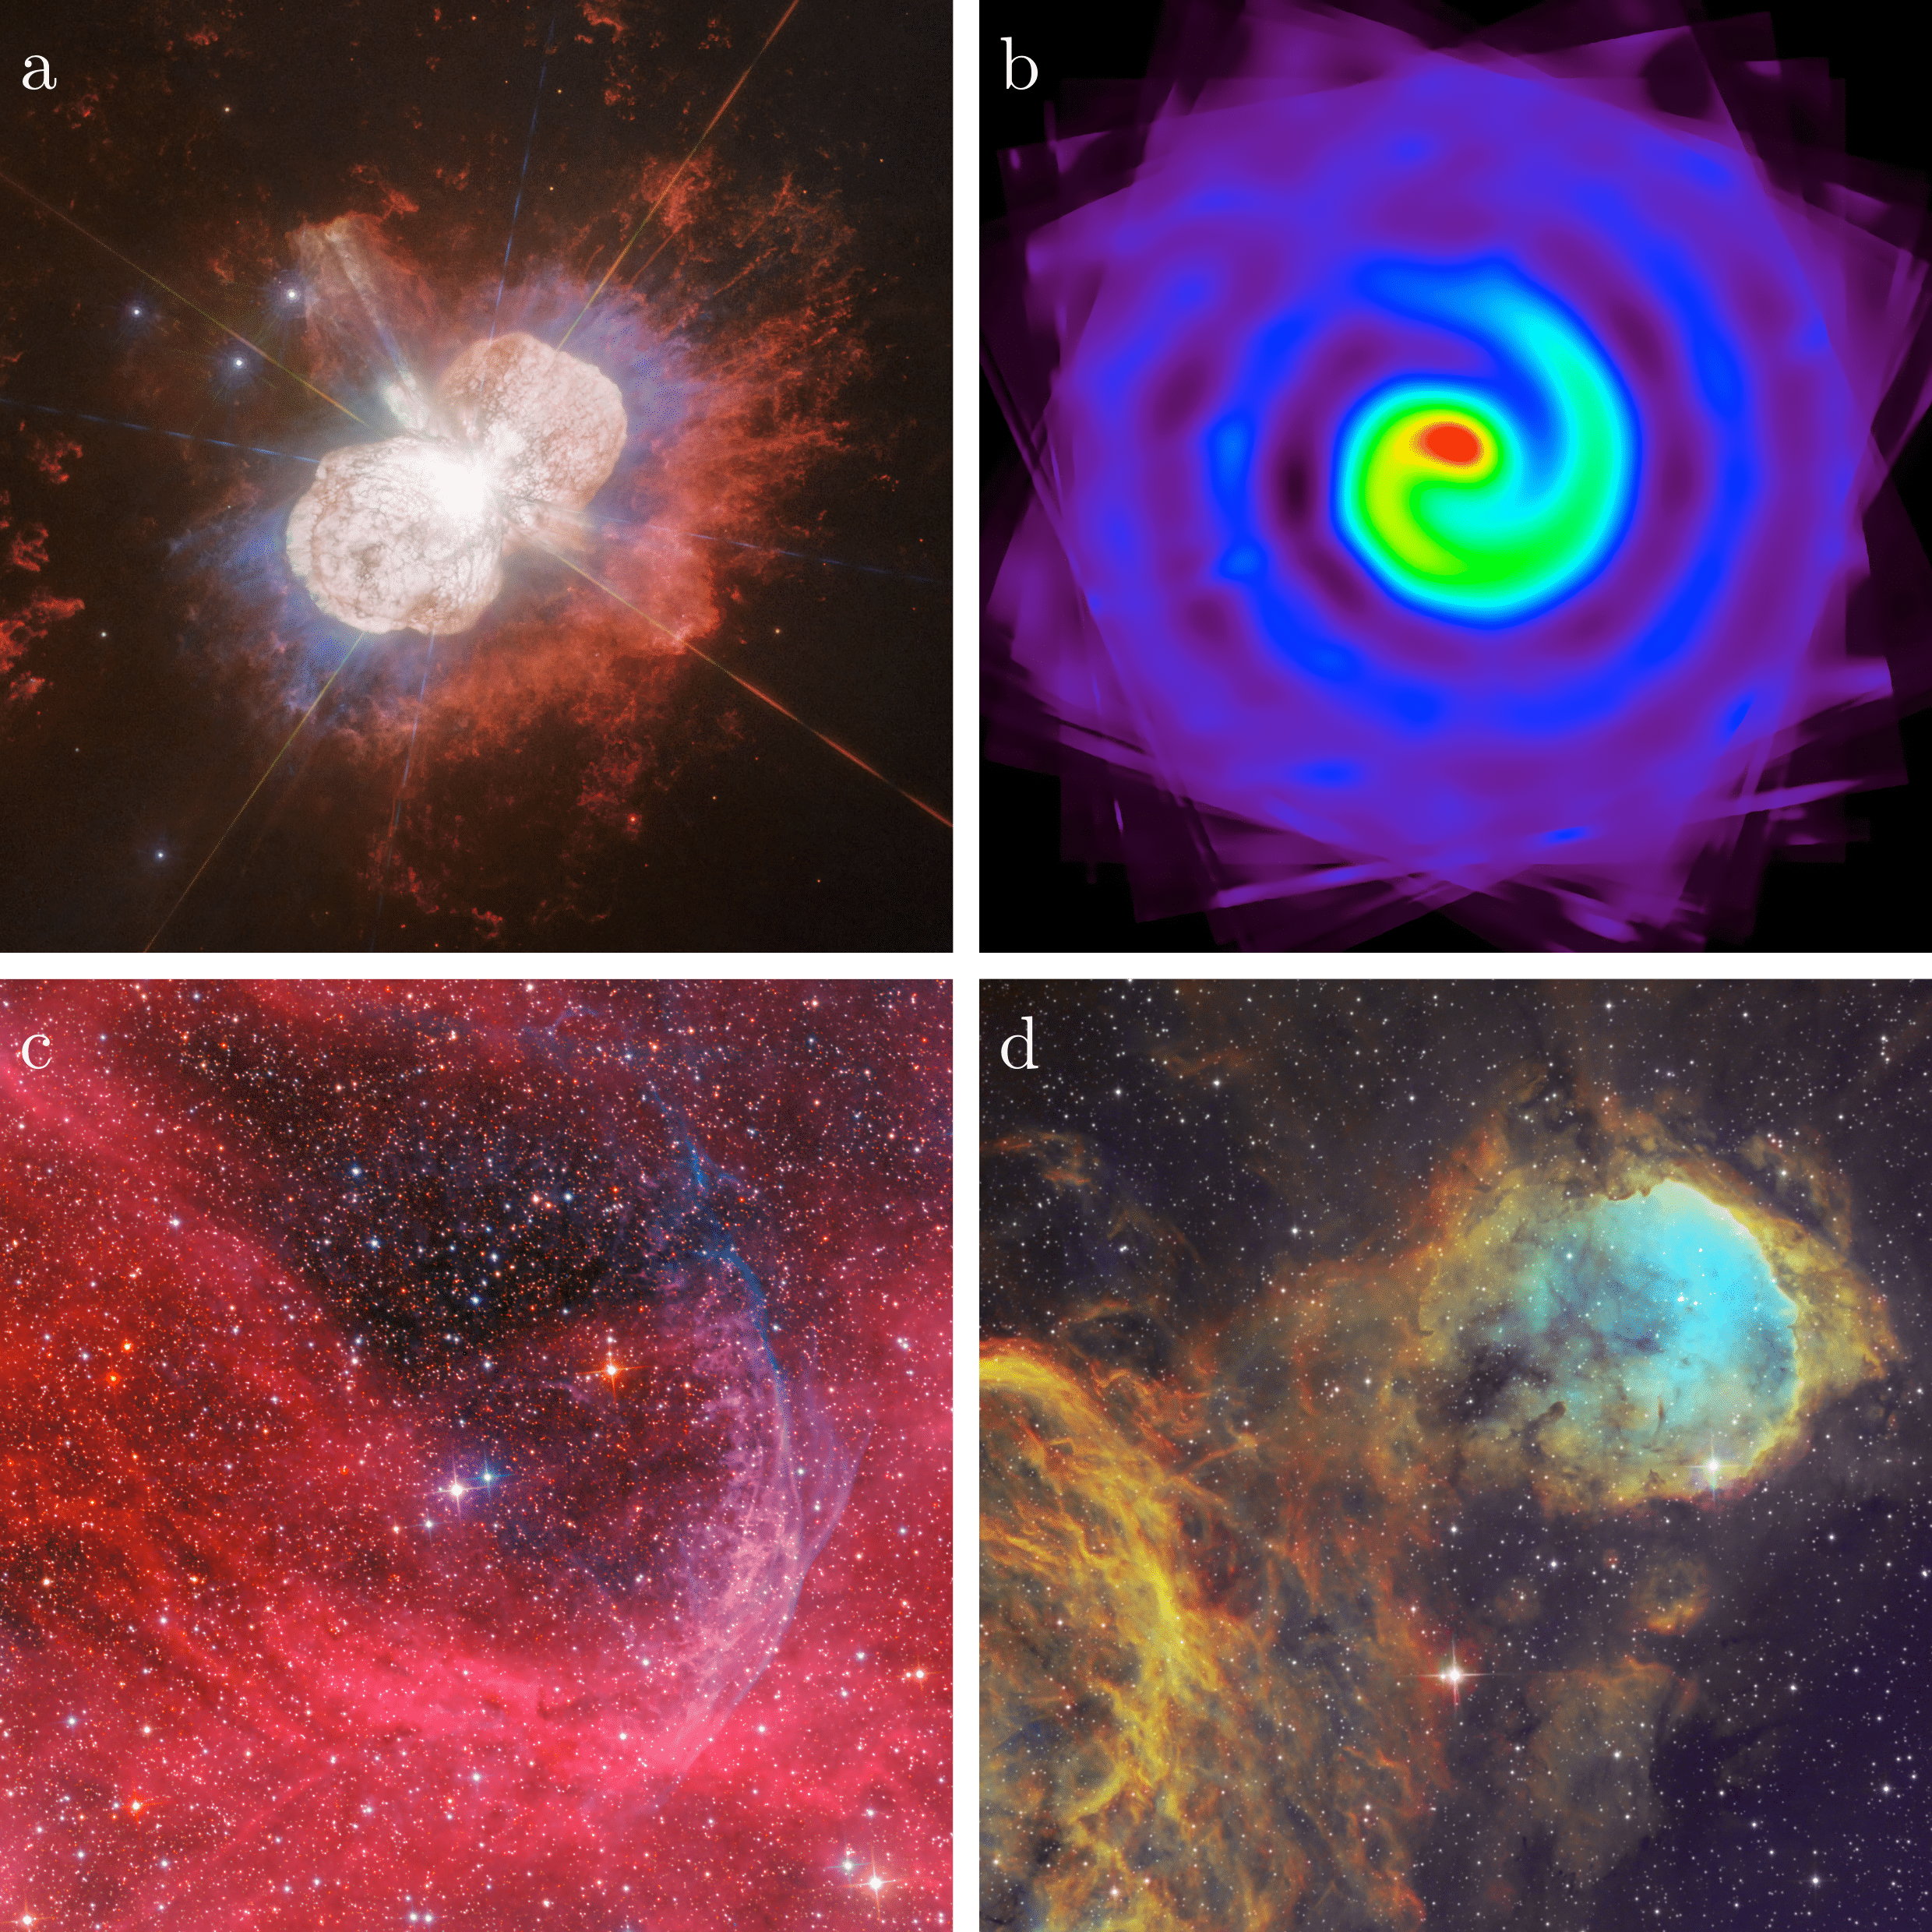
\includegraphics[width=5in]{assets/wolf-rayets/wolf-rayets.png}
  \caption[NASA APOD images of Wolf-Rayet and CWB systems]{NASA Astronomy Picture of the Day (APOD) images of Wolf-Rayet and CWB systems. (a) The LBV+O system $\eta$ Carinae (\link{https://apod.nasa.gov/apod/ap190220.html}). (b) The persistent dust forming colliding wind binary (WCd) system WR 104 (\link{https://apod.nasa.gov/apod/ap140603.html}). (c) The WR134 ring nebula (\link{https://apod.nasa.gov/apod/ap120621.html}). (d) The Wolf-Rayet nebula surrounding WR23 (\link{https://apod.nasa.gov/apod/ap210208.html}). Wolf-Rayet and CWB systems are, without a doubt, some of the most striking systems in the galaxy.}
  \label{fig:cwbexamples}
\end{figure}

Colliding Wind Binary (CWB) systems are perhaps one of the most striking types of stellar system.
% Notes on beauty
Beauty, as they say, is in the eye of the beholder -- and nearly every astrophysicist believes that parts of their specialist subjects hold tremendous aesthetic qualities.

Figure \ref{fig:cwbexamples}, however, really does show off the intrinsic beauty of both Wolf-Rayet (WR) and the much rarer CWB systems.

These systems can produce a variety of beautiful outbursts.
From Wolf-Rayet nebulae, to delicate interstellar dust clouds forming around them in the infrared.
The latter form either fine filaments, or pinwheels extending out for parsecs, with an enormous amount of structural variety.
On top of the visible and infrared, these systems are also visible from the radio to gamma rays, emitting copious amounts of radiation though both thermal and non-thermal mechanisms.

Massive stars on the whole have an incredibly outsized influence on their local interstellar medium (ISM).
Even in a single system, these stars produce winds capable of perturbing their local medium, forming pockets of high density material that can drive star formation, as well as ionising this medium, producing HII regions.
Wolf-Rayet (WR) stars turn the metaphorical dial of this influence up to 11, driving enormous quantities of hot, ionised wind into the ISM.
These stars literally tear themselves apart over a period of around 500,000 years, flinging many solar masses worth of material into space at an appreciable fraction of the speed of light.
These stars too, are destined to die in violent, chaotic, and beautiful\footnote{Provided you are not in the blast radius.} ways, such as supernovae and gamma-ray bursts (GRBs).

If these stars form a close binary with colliding winds we observe incredibly powerful shocks, as the mechanical energy equivalent to the luminance of a thousand suns acts on a region only a few solar radii in size.
This heats this wind collision region (WCR) to temperatures in excess of $10^8 \, \si{K}$ as these winds crash headlong into each other.
These systems are among the brightest continuous x-ray sources in the night sky (Fig. \ref{fig:intro-xray}), and provoked much scientific debate before the discovery of their true nature. 

\begin{figure}[ht]
  \centering
  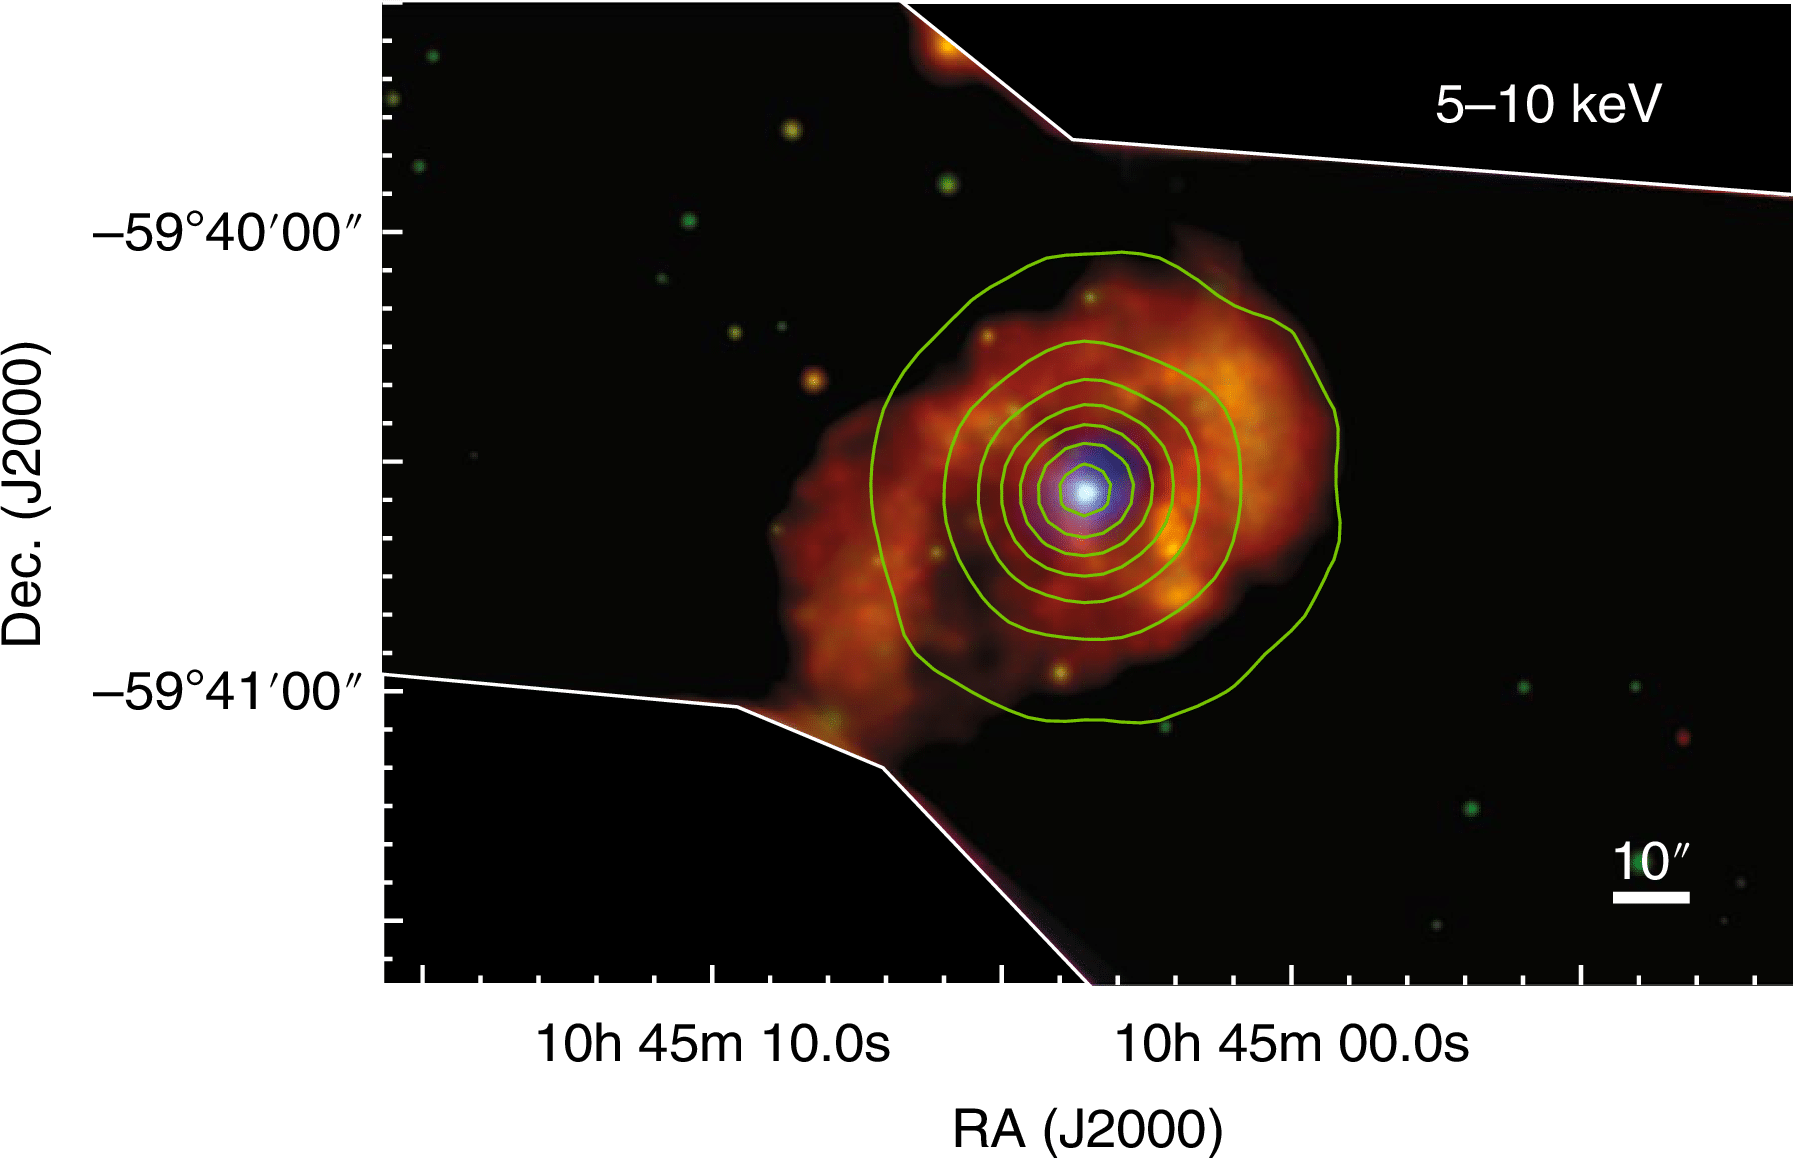
\includegraphics[width=4in]{assets/wolf-rayets/x-ray.png}
  \caption[\emph{Chandra \& NuSTAR imagery of $\eta$ Carinae \parencite{hamaguchiNonthermalXraysColliding2018}}]{Chandra x-ray imagery of $\eta$ Carinae at the soft x-ray minimum of 2009, with contours from the NuSTAR $5-10 \, \si{\kilo\electronvolt}$ x-ray band. CWB systems are incredibly bright in x-ray bands due to the powerful shock heating driving thermal x-ray processes. Image sourced from \textcite{hamaguchiNonthermalXraysColliding2018}.}
  \label{fig:intro-xray}
\end{figure}

However, the most puzzling question is how dust forms in certain CWB systems (so-called WCd systems).
These systems have violent shocks, incredibly high temperatures, and produce copious amounts of ionising radiation, so how can it be that something as tenuous as interstellar dust can form?
The mechanisms behind formation and growth are extremely poorly understood, and as such we intend to glean some information on the mechanisms and yields of dust production processes in these systems.

\section{Motivation \& Goals}
\label{sec:projectgoals}

% Initial motivation
Dust formation in early-type star systems is a relatively poorly understood phenomenon.
As the grains should be readily destroyed by shocks and ionising radiation, this requires some form of shielding or additional dust growth mechanisms.
% Point of dust formation
We find that these systems -- if in a binary -- can produce volumes of dust equivalent to asymptotic giant branch stars, the most prolific late-type dust forming systems.
Dust formation is also vital for the formation of planets and complex organic molecules throughout the galaxy, so understanding the mechanisms behind its formation is of significant scientific interest.
% Stellar feedback and massive stars 
CWB systems are -- for a variety of reasons -- very difficult to both observe \emph{and} simulate.
CWB systems are typically quite distant, with the nearest systems being approximately \SI{2}{\kilo\parsec} from Earth, making the wind collision region (WCR) very difficult to observe.
The WCR is also shrouded by dense stellar winds, occluding the shock region.
These systems are also comparatively rare, making it more difficult to typify these systems.
If we simulate these systems, we find other difficulties such as a requirement of 3D simulation in order to model orbital effects.
These systems also have a large variation in length scales that render the simulations very computationally challenging.

% Development of a dust model
The main goal of the project was to develop a dust model that was computationally inexpensive to implement, such that it could be included in large-scale numerical models 

% Broad outline of feature set, link to sections
This dust formation model\footnote{Christened \bidmas{}, or binary interaction dust model with accretion and sputtering.} was designed to be as modular as possible, and to be relatively straightforward to implement additional dust evolution mechanisms.
By the end of the project, dust evolution and destruction mechanisms were implemented, as was dust cooling through gas-grain collisional excitation.

% MOdel two types of system
The second goal of the project was to simulate a variety of WCd systems using this dust model running within a hydrodynamical simulation.
WCd systems can be sub-categorised by the time dependence of their dust formation:

\begin{itemize}
  \item ``Episodic'' systems that produce dust over a small section of their orbit. 
  \item ``Variable'' systems whose dust production varies significantly over their orbital period.
  \item ``Persistent'' systems whose dust did not vary significantly over the orbital period.
\end{itemize}

\noindent
It was intended from the beginning of the project to observe at least two of these systems, with the work on each system constituting a journal paper.
% Overall, two such systems archetypes, variable and episodic, were simulated.
% Persistent dust forming systems -- WR98a

The first type of WCd system observed was the variable dust forming system WR98a.
We found that this system was the easiest to simulate, due to its comparatively sedate winds and larger orbital spacing. 
% Parameter space search 
In addition to simulating a system with parameters similar to WR98a, a parameter space search was conducted using WR98a as a baseline, wind properties predicted to be influencing the dust production rate were varied, in order to understand their effects.
% Episodic dst forming systems -- WR140
The episodic dust forming system WR140 was also simulated, whose dust formation is theorised to be due to its high orbital eccentricity.
This was a more complex affair, as the system was far more complex to simulate than WR98a.
This section of the project had to be partially truncated due to time constraints, and a partial orbit of the system near periastron was opted for in lieu of a full orbit of the system.

% Missed opportunities, time limitations
It should be noted that there were a number of technical difficulties throughout the project, and as such, a lot of the project was conducted on a very time-constrained basis.
Whilst the main goals of the project were completed, there is still much that is not understood about dust formation in these systems.
Development of a more complex model, as well as synthetic astronomical imaging through radiative transfer models were topics considered for later stages of this project but could not be accomplished due to time.
However, these projects present interesting avenues of future research.
Other wind features, such as radiative line driving, would also be included in future models, in order to understand their role in dust formation, and how they influence grain growth and dust yields.
Furthermore, simulation of other systems, such as the WR+WR systems WR70-16 ``Apep'' and WR48a would be interesting follow-up simulation targets.

\section{Thesis Structure}

The structure of this thesis could be described as somewhat unconventional, this is because of two primary reasons:

\begin{itemize}
  \item Difficulties in the early and middle sections of the project.
  \item The field itself requiring a significant degree of explanation.
\end{itemize}

\noindent
Throughout the \nth{2} and \nth{3} years of this PhD, there were many issues with getting this project to progress at all.
This was mostly due to failing to get the original hydrodynamical code used in this experiment to work.
This code was ultimately abandoned by the \nth{3} year and replaced with a more modern and easier to develop code, \athena{} (Sections \ref{sec:mgcode} \& \ref{sec:athenapp}).
Additionally, the outbreak of a global pandemic put a significant degree of stress on the work, and meant that there was a lot of time to develop the codebase and theorise on the nature of these systems; but much of the actual data collection was performed in the last few months of the project.
As such, there is a great deal of discussion of the background and methodology, and an enormous amount of discussion on the future of this particular field.
While the primary objectives of this PhD were achieved, many aspects of this work that were laid out at the start of the project were unfortunately truncated or removed.
This was extremely disappointing, of course, but I hope to continue work on this field outside of this PhD, and develop a more advanced dust model for numerical simulation.

% Two introductory sections
Astrophysical fluid dynamics straddles two particularly complex fields, physics and computer science.
Unfortunately universities don't award two PhDs for work involving this subject, instead we have to discuss these two fields at great length.
Because of this, the first two chapters of this thesis are both background chapters\footnote{A friend of mine wrote their thesis on computational biophysics that had not one, not two, but \emph{three} background chapters, so it could be worse.}.
In Chapter \ref{ch:background} we discuss the physics of massive stars and dust, before synthesising these two sections in order to discuss dust producing CWB systems.
Whereas in Chapter \ref{ch:numsim} we will discuss the underlying principles of numerical simulation, and discuss our model, from the choice of numerical code to the underlying mechanisms and methodology.
% Paper chapters
Afterwards, we will move on to Chapters \ref{chap:parameterspace} \& \ref{ch:wr140}.
These chapters have been adapted from two papers written concurrently with this thesis:

\begin{enumerate}
  \item \emph{\firstpapertitle} \turbo{Include first paper citation}.
  \item \emph{\secondpapertitle} \turbo{Include second paper citation}.
\end{enumerate}

\noindent
These chapters serve to provide more concise explanations of our work, while also providing the results of this research, particularly dust formation rates of both persistent and episodic WCd systems.
Finally, we will conclude with some remarks on future work that could be performed in this field, as well as with some observations made over the course of this project.
\chapter{Background}

\section{Early-Type Stars}
\label{sec:earlytype}

%//TODO I quite like this joke but it needs a bit of work
The term Early-type stars is quite possibly the epitome of bad naming conventions in astrophysics, it's a very old term, coming from the dawn of astrophysics itself, quite opaque as to what it means, and also by definition \textit{completely wrong}. In fact it is one of the most wrong pieces of terminology I can think of.\footnote{Aside from astrophysicists calling something ``warm'', of course. That can quite literally mean anything from 10 to 10,000 Kelvin, depending on who you ask, what they're writing about, or how they're feeling at that particular moment. In fact, I'll probably end up falling into this same trap somewhere in this thesis as well!}
The first generation of astrophysicists found themselves asking very important questions such as ``what even \textit{are} stars?'' and ``what possible mechanism can allow a star to burn for so long?'' Each of these questions was rather pressing for the burgeoning field, and the scientific community was aching for an answer.

Of course, like all pressing questions of the \nth{19} century, it fell to Lord Kelvin to provide a convincing but incorrect answer. Kelvin assumed that gravitational collapse was the mechanism for a stars long-term heating, with younger, ``early'' type stars shining the brightest. Not only was the mechanism incorrect, but typically older main sequence stars are more luminous than their younger counterparts of a similar mass! However, as is the case with astrophysical terminology, the term stuck, to the confusion of many young astrophysicists.

%//FIXME POTENTIAL maybe put this part in with OB stars? allows for more seamless switching from diatribe to the main body

Instead, we now know that stars produce their energy through fusion. These reactions vary from sub-stellar deuterium and lithium burning, to main sequence p-p \& CNO hydrogen burning processes, and finally to the triple-$\alpha$ and other exotic fusion processes for evolved massive stars. The more massive the star the greater the internal pressure, allowing for more exotic fusion processes.
The bigger a star, the greater the core pressure and temperature, as all fusion reactions are highly dependent on temperature, stars with only a few dozen solar masses are thousands of times more luminous than our sun, but only live a fraction of the time \parencite{carrollIntroductionModernAstrophysics2014}.

\subsection{OB-type stars}
\label{sec:obtype}

And with that we shift our gaze to high-mass stars, with the most massive of all being the O and B type stars, these are extremely luminous ($\sim 10^4 \,\si{\solarluminosity}$), and relatively short lived ($\sim 10 \, \si{\mega\year}$) stars. The age-old adage of a candle burning twice as bright lasting half as long applies to our studies of the cosmos, but it is more apt to compare a candle and a stick of dynamite when considering stars on opposing ends of the Harvard classification system.

% Formation of OB stars, note binary systems!

The most common formation mechanism of stars is through the collapse of a giant molecular cloud\footnote{GMC}, an enormous cool cloud many parsecs across with a mass of around $10^4 \si{\solarmass}$.
As this GMC collapses and radiates energy, lowering the radius of thermostatic equilibrium for the cloud, as collapsing progresses the cloud fragments into many smaller regions with a critical density, capable of collapsing further, forming a star.
The collapse of a GMC can be described with a series of timescale.
First, the Kelvin-Helmholtz timescale, $\tau_{KH}$, which describes the timescale required for the radiating cloud to collapse.
The second important timescale is the free-fall timescale, $\tau_{ff}$, which is the time taken for a cloud to collapse. These timescales are described by the following equations:

\begin{subequations}
  \begin{align}
      \tau_{KH} & \approx \frac{GM_*^2}{R_*L_*} \label{eq:khtime} ,\\
      \tau_{ff} & = \sqrt{\frac{3\pi}{32G\bar{\rho}}} \label{eq:fftime} ,
  \end{align}
  \label{eq:khfreefalltimes}
\end{subequations}

where $M_*$ is the protostellar mass, $R_*$ is the protostellar radius, $L_*$ is the protostellar luminosity, and $\rho$ is the mean density of the collapsing cloud \parencite{ward-thompsonIntroductionStarFormation2011}.

%//TODO is the above section completely necessary? it might be better to just describe star formation.

Perhaps the most important distinction between massive star formation and its better understood counterpart is as a young protostar approaches the main sequence, the KH timescale is less than the free-fall timescale, meaning the material at the center of the collapsing cloud begins fusion while the bulk of core has collapsed onto the site of the future star. This burgeoning star begins to drive the weakly gravitationally coupled collapsing material away due to its sheer luminosity, driving this material outwards, causing it to accrete and shock material within the GMC. 

Another important consideration is the role of angular momentum as the star collapses.
The particularly massive cloud involved in massive star formation is more prone to fragmentation, meaning that massive stars typically form with an orbital partner, whilst approximately 2/3\textsuperscript{rds} of low-mass stars are part of a binary or multiple system, this value is near-total.
As such, the environment within an OB association after star formation consists of numerous young stars in tightly-knit groups disrupting the entire local area.\footnote{This is a bit like living in Headingley, Hyde Park, or any other area with lots of Undergraduates.}

%//TODO cite "near total" statistic, it's in one of the more recent papers you've had a look at, maybe a williams one?

Above a stellar mass of $1.3 \si{\solarmass}$ pressures and temperatures within a stellar core favour the fusion of hydrogen into helium through the catalytic CNO cycle, instead of the more direct p-p fusion process. 

\begin{subequations}
  \begin{align*}
    \prescript{12}{6}{C} + \prescript{1}{1}{H} & \rightarrow \prescript{13}{7}{N} + \gamma \\ 
    \prescript{13}{7}{N} & \rightarrow \prescript{13}{6}{C} + e^+ + \nu_e \\
    \prescript{13}{6}{C} + \prescript{1}{1}{H} & \rightarrow \prescript{14}{7}{N} + \gamma \\
    \prescript{14}{7}{N} + \prescript{1}{1}{H} & \rightarrow \prescript{15}{8}{O} + \gamma \\
    \prescript{15}{8}{O} & \rightarrow \prescript{15}{7}{N} + e^+ + \nu_e \\
    \prescript{15}{7}{N} + \prescript{1}{1}{H} & \rightarrow \prescript{12}{6}{C} + \prescript{4}{2}{He} 
  \end{align*}
\end{subequations}
%//FIXME sort out italics, use regular fonts
%//TODO add net energy gains losseslosses
%//TODO Check to see if this is correct


%//FIXME mechanism less efficient, 0.6MeV per nucleon, but reaction rate just quite a lot faster, temperature sensitivity, series of power laws, t^40 for 1e8k and t^20 for 2e8k
The reaction rate of CNO rises much faster, resulting in a convective core, surrounded by a radiative envelope \parencite{salarisEvolutionStarsStellar2005}. This is the driving force behind the incredible luminosities of an OB star as it hurtles along the main sequence.

%//TODO might be a good idea to include that one graph with fusion rates?

% Influence of OB stars on surrounding environment, outsized influence etc.

% Touch on stellar winds, expand in next section

% Evolution and fate of massive stars, evolution, depletion of hydrogen products, then onto helium burning

Unfortunately for massive stars, pesky fundamental laws such as the conservation of energy come into play. With only an order of magnitude or two of additional mass more than our sun and shining $10^4$ times as brightly, this curtails the life of the brightest stars to lifespans not much more than $10^7$ years.
If we define a galactic year as the time it takes for a star to orbit the Milky Way, these poor stars don't even make it to their first birthdays, which is quite sad really.\footnote{Continuing this analogy our sun can drink, might have voted if they felt like it, and may be racking up vast quantities of student debt.}


As the available hydrogen begins to become depleted, the lowering reaction rates force the star to shrink, this raises the internal temperature until the core begins to burn helium through the triple-$\alpha$ process:

\begin{subequations}
  \begin{align*}
    \prescript{4}{2}{\text{He}} + \prescript{4}{2}{\text{He}} & \rightarrow \prescript{8}{4}{\text{Be}} \\
    \prescript{8}{4}{\text{Be}} + \prescript{4}{2}{\text{He}} & \rightarrow \prescript{12}{6}{\text{C}} + 2\gamma
  \end{align*}
\end{subequations}

The sudden spike in energy radiating from the core shifts the calculus of hydrostatic equilibrium in the favour of outward forces, causing the star to rapidly expand in the form of a Red Supergiant or Luminous Blue Variable \parencite{ryanStellarEvolutionNucleosynthesis2010a}.
During this phase the energy output of the star is even greater, with a timescale of $\sim 10^6$ years, this is only temporarily prolonging the life of the star, which will inevitably begin burning heavier and heavier elements, faster and faster.
Once the star starts producing iron its fate is sealed, the star stops fusing, and collapses, annihilating itself in the form of a supernova and leaving behind a remnant of its core in the form of a neutron star or black hole 
\parencite{ward-thompsonIntroductionStarFormation2011}.

Whilst the stars end is as inevitable as it is violent, the intermediate stage as the star leaves the main sequence is in itself extremely interesting, and for the context of this thesis, no product of this stage is more interesting than the Wolf-Rayet.



\subsection{Wolf-Rayet stars}
\label{sec:wrtype}


%Notes: Evolution type 
% Jumping off point, wiki wolf-rayet current models, research papers therein
% For WC formation O->RSG->WNE->WC 20-45 msol
% WR in general O->LBV->WR

% History and background of Wolf-Rayet stars

% Description of Wolf-Rayet star, introducing concept of strong stellar wind

As we now know, Wolf-Rayets\footnote{Abbreviated to WR.} are evolved forms of O-type stars, and are a short lived component of the life-cycle of massive stars, typically lasting for around \num{5e5} years \parencite{crowther_physical_2007}.
Despite this relatively transient length of this stage, the influence of a WR star on its local medium is extremely outsized.
WR stars in particular are known for having dense, fast winds, typically between 2 and 3 orders of magnitude than their main sequence O-type progenitors, with mass loss rates on the order of $10^{-5} \, \si{\solarmass\per\year}$ and wind velocities of $\num{1.5e3} \, \si{\kilo\metre\per\second}$.
This extremely dense wind is driven by the highly energetic helium burning core, which is luminous enough as to drive away the outer layers of the stars envelope, exposing the core.
The observed spectroscopic lines are due to heating of the envelope from the core, which is enriched with by-products of hydrogen and helium burning, the lack of hydrogen lines is due to the stars evolved nature, as all the hydrogen has been burned, there is simply nothing left to observe!

%Subcategorising wolf-rayets into WN, WC and WO

Wolf-Rayet stars can be subcategorised through spectroscopic observation, which indicates enrichment in a particular element, the 3 major sub-types, WN, WC and WO are defined by their strong nitrogen, carbon and oxygen lines respectively.
The important distinction between WN and WC/WO stars is that WN stars are enriched through hydrogen burning, whilst WC and WO are enriched through the by-products of helium burning \parencite{vinkVeryMassiveStars2015}.

% WR star subcategorisation and evolution
As a Wolf-Rayet continues to lose its envelope, additional products of fusion processes are dredged up from the centre of the star.
In the case of the WN sub-type, the broad nitrogen lines correspond to the outer layer of the envelope, enriched through the CNO process; after this outer envelope is cast off, the remainder of the envelope exhibits carbon and oxygen lines, indicating enrichment from the triple-$\alpha$ process.
Finally, the star evolves further and the innermost region of the envelope is revealed, observed as the strong oxygen lines of a WO sub-type \parencite{neugentWolfRayetContent2019,oswaltPlanetsStarsStellar2013}.

%//TODO this needs rewriting

As an O-type star transitions to a Wolf-Rayet, it typically undergoes an intermediary LBV or RSG stage as helium burning begins, this is mass dependent, with the various transitional states described by \cite{crowther_physical_2007}:

\begin{subequations}
  \begin{align*}
    \text{O} \rightarrow \text{LBV/RSG} \rightarrow \text{WN(H-poor)} \rightarrow \text{WC} \rightarrow \text{SN 1b} & ,~~ \text{for } 25 \, \si{\solarmass} < \text{M}_{\text{WR}} < 40 \, \si{\solarmass} \\
    \text{O} \rightarrow \text{LBV} \rightarrow \text{WN(H-poor)} \rightarrow \text{WC} \rightarrow \text{SN 1c} & ,~~ \text{for } 40 \, \si{\solarmass} < \text{M}_{\text{WR}} < 75 \, \si{\solarmass} \\
    \text{O} \rightarrow \text{WN(H-rich)} \rightarrow \text{LBV} \rightarrow \text{WN(H-poor)} \rightarrow \text{WC} \rightarrow \text{SN 1c} & ,~~ \text{for } \text{M}_{\text{WR}} > 75 \si{\solarmass} 
  \end{align*}  
\end{subequations}

%//TODO add binary formation mechanism paragraph

% subcategorisation through numerical system

%//TODO include table of approximate mass loss rates, numerical classification

% Wolf-Rayets in a binary
Wolf-Rayet stars are important in the context of this work due to their outsized influence within a WR+OB binary pair.
The WR component of a WR+OB binary has an outsized contribution in returning material to the ISM, whilst also dominating the dynamics of the system, with their winds completely overpowering those of their O-type neighbours.
In some cases, the dense, fast wind from the WR can collide with the much more tenuous wind from its partner, forming a strong shock, and a variety of fascinating effects.
However, I wouldn't want to spoil too much too soon, but you can skip ahead to section \ref{sec:cwb}, where this phenomena is covered in more detail.
%//HMM This may be a bit too jovial!


\section{Stellar Winds}
\label{sec:winds}

% Section covers wind driving mechanisms, while wind is touched on in the previous section, this covers the mechanisms more thoroughly

Stellar winds have already been discussed to some extent in the previous section, however, due to the significance of winds within this body of work, further detailing of winds must be discussed to gain a better understanding of the dynamics of Colliding Wind Binary systems. This section will cover in brief the study of stellar winds, particularly driving mechanisms from low and high mass stars.

% Background of stellar winds, particularly history of the subject

% Define the mass loss rate, mdot
% Single wind estimates and densities

%Define the terminal velocity, discuss why this may not be completely accurate

The study of stellar winds is of course, rather hard from our vantage point on Earth, as direct observation of a non-stellar solar wind is difficult, and sampling of the winds themselves significantly more difficult than that due to the inconvenient distances involved in interstellar travel.
Because of this, extrasolar wind properties are derived from spectrography, with velocities derived through Doppler shift.
The important parameters to consider in a wind, especially for this thesis, is the mass loss rate, $\dot M$, the wind terminal velocity, $v^\infty$ and the abundances within the wind.

%https://www.ifa.hawaii.edu/users/kud/windsfromhotstars/hotwinds.html

\begin{equation}
  \frac{dM}{dt} = 4 \pi \rho(\boldsymbol{r}) v(\boldsymbol{r}) \boldsymbol{r}^2, \label{eq:massloss}
\end{equation}

\begin{equation}
  \rho_w = \frac{\dot{\text{M}}}{4 \pi v^\infty r^2}, \label{eq:smoothwind}
\end{equation}

This section will cover the different driving mechanisms winds from low and high mass stars, the typical wind parameters and driving mechanisms are broken down in table \ref{tab:windcomp}.


\subsection{Stellar winds in low mass stars}
\label{sec:lowmasswinds}
% Introduction, refer to table


% Low mass main sequence

Low mass stellar main sequence stellar winds are quite paltry for an astrophysical phenomenon, the sun, for instance, drives thin, comparatively slow winds, with a mass loss rate of $\sim 10^{-14}$ \si{\solarmass\per\year} and a terminal velocity of 400 \si{\kilo\metre\per\second}. The mechanism behind this is gas pressure from coronal heating, with outward pressure driving gas within stellar atmosphere away from the star, this results in a transonic wind that quickly reaches its terminal velocity as the coronal temperature and subsequent pressure quickly drops off.

% Short section on red dwarf winds

% Off the main sequence, dust driven winds

As a low mass star exits the main sequence, ballooning in size to become a red giant, the density of the stellar wind increases dramatically. 

As dust condenses in the upper atmosphere of the red giant, these grains can readily adsorb photons, utilising radiation pressure to be driven away from the more luminous giant star, easily achieving escape velocity against the low surface gravity of the red giant.
Gas is also driven away, coupled to the dust, this provides an efficient form of momentum transfer, allowing for an extremely dense albeit slow stellar wind

\label{sec:dustdriven}

\subsection{Stellar winds in high mass stars}
\label{sec:radlinedriving}

In the same way that high-mass stars are many orders of magnitude brighter than their low mass counterparts despite a comparatively low increase in mass, the same can be said of the density of stellar wind. A main sequence OB star typically has a mass loss rate of $10^{8}$ \si{\solarmass\per\year}, 6 orders of magnitude higher than a solar mass star.
This discrepancy in wind density cannot be explained by stronger coronal heating, in fact, the lack of a convective envelope ensures that coronal heating is not even feasible as a driving method!
Instead we must look towards the higher luminosities that massive stars exhibit to find a suitable mechanism.

Simple radiation pressure from these stars would not be enough to explain the observed dense, highly supersonic winds emanating from these massive stars.

Resonance lines were also considered, a photon with an energy equal to the excitation energy of an ion is absorbed by that ion, gaining the momentum of this ion.
The ion subsequently de-excites over a timescale on the order of $10^{-8}$ \si{\second}, emitting a photon at a random angle relative to the radial direction, $\alpha$. The resultant change in radial velocity, $\Delta v_r$, for the adsorption of a photon at the resonance frequency $\nu_0$ is

\begin{equation}
  \Delta v_r = v''_r - v_r = \frac{h\nu_0}{mc} (1-\cos\alpha),
\end{equation}

where $v''_r$ is the radial velocity after the absorption and emission events, and $m$ is the ion mass.
These ions are accelerated away from the star, along with the rest of the stellar wind which is coupled through Coulomb forces.
The opacity of such resonance lines can be up to six orders of magnitude larger than the opacity of a Thomson scattering event \parencite{lamersIntroductionStellarWinds1999}. Additionally, this effect is not observed in low-mass stars, whose spectra typically peak in the visible light, while resonance lines typically have energies equivalent to UV photons (figure \ref{fig:planck-comp}).
O-type stars and Wolf-Rayets, however, emit much of their radiation within the UV range.

\begin{figure}
  \centering
  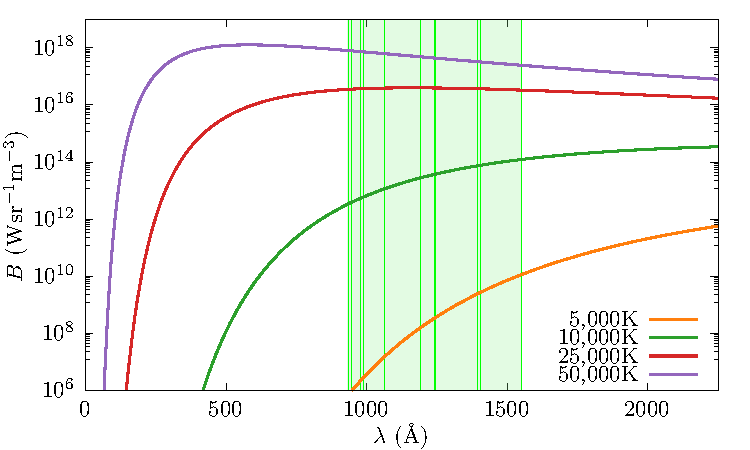
\includegraphics{assets/plancks-law/plancks-law.pdf}
  \caption[Planck's law radiance comparison with resonance lines]{Spectral radiance against wavelength for black body objects at various effective temperatures, $T_{\text{eff}}$, a series of wavelengths corresponding with important resonance lines in table 1 of \cite{lucy_mass_1970} have been included. As temperature increases the spectral radiance at resonance line wavelengths dramatically increases, with a minimum of 6 orders of magnitude difference between the effective temperatures of a solar equivalent main sequence star and an O-type main sequence or Wolf-Rayet star.}
  \label{fig:planck-comp}
\end{figure}

% Need to briefly explain P-Cygni profiles as well

% Radiative line driving, this section may need to be beefed up

Early computations involving resonance lines from \cite{lucy_mass_1970} provided a more reasonable mass loss rate calculation, but were still off by approximately two orders of magnitude.
Building off of the work by Lucy \& Solomon, a vital paper in the solidification of radiative lines as the main driving mechanism behind massive star outflows was produced by Castor, Abbott and Klein\footnote{Hereafter abbreviated as CAK.}.
The CAK formalism calculated reasonably close wind velocities, while being accurate to within a factor of 3 for mass loss rates \parencite{castor_radiation-driven_1975}.
Further work allowed for more accurate computations of the line driving effect, such as the mCAK prescription, the Sobolev approximation and the finite disk correction factor \parencite{pauldrachRadiationdrivenWindsHot1986}.

% Evolved OB stars, WR stars

As previously mentioned, evolved massive stars progress into a helium burning WR phase, at this point, mass loss rates due to radiative line driving are extreme, in the order of $10^{-5}$ \si{\solarmass\per\year}.
This outsized influence on the local medium can be seen in the production of ejecta nebula, such as M1-67 produced by WR 124 (figure \ref{fig:wr124}).

%//FIXME this is a placeholder, additionally how should I cite this?
\begin{figure}[h]
  \centering
  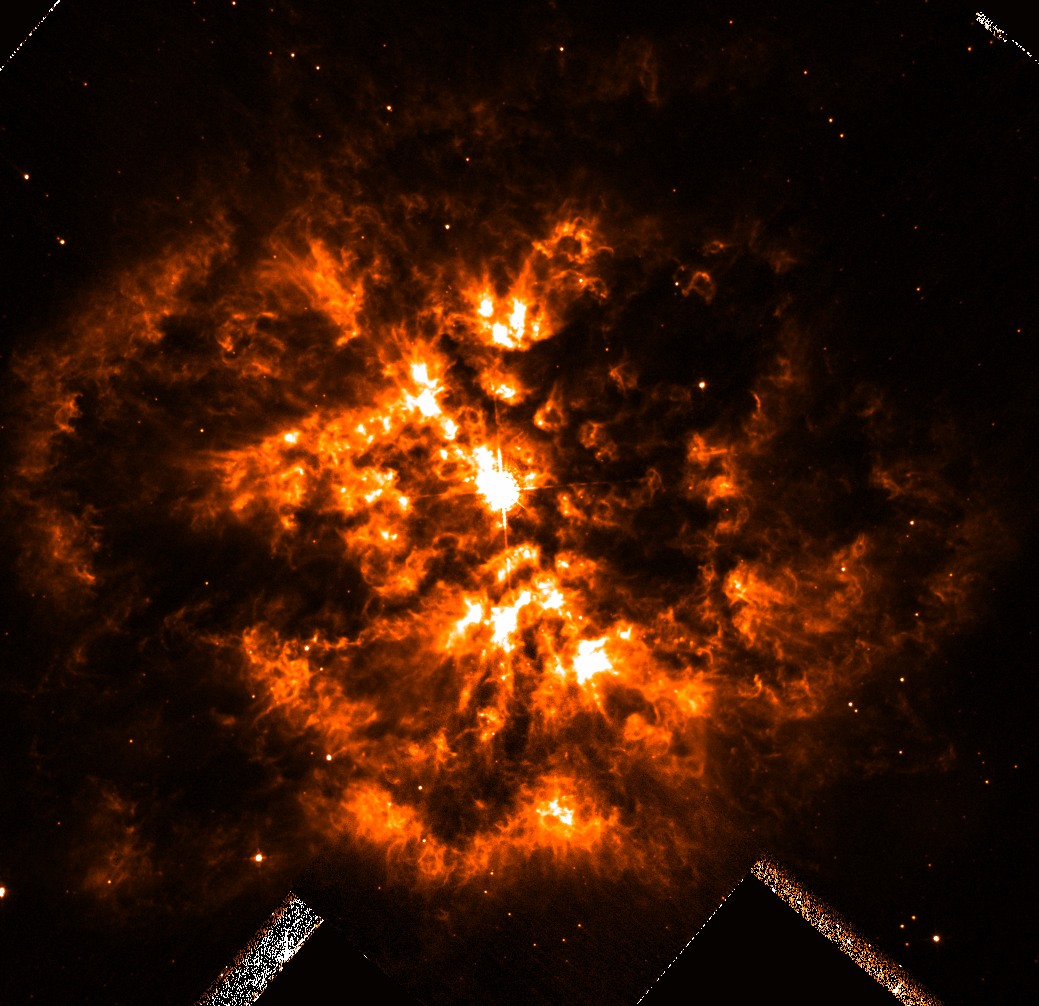
\includegraphics[width=4in]{assets/WR124.png}
  \caption[\textit{M1-67 nebula around WR 124 \parencite{2010ApJ...724L..90M}}]{Reduced Hubble WFPC2 data of the WN star WR 124, its extreme mass loss is currently producing the ejecta nebula M1-67 \parencite{2010ApJ...724L..90M}.}
  \label{fig:wr124}
\end{figure}

\begin{table}[h]
  \centering
  % \resizebox{\textwidth}{!}{%
  \begin{tabular}{cccc}
  \hline
  \multicolumn{1}{c}{Star} & \multicolumn{1}{c}{$\dot M$} & \multicolumn{1}{c}{$v_\infty$} & \multicolumn{1}{c}{Mechanism} \\
  \multicolumn{1}{c}{}     & \multicolumn{1}{c}{$\si{\solarmass\per\year}$}         & \multicolumn{1}{c}{$\si{\kilo\metre\per\second}$}           & \multicolumn{1}{c}{}          \\ \hline
  Sun            & $10^{-14}$        & 400  & Thermal heating \\
  Pre Main Sequence & $10^{-4}-10^{-7}$ & 200-500 & Rotation \& magnetic fields \\
  Red Giant      & $10^{-7}-10^{-9}$ & 30   & Radiation pressure on dust grains        \\
  OB Star        & $10^{-7}-10^{-8}$ & 2500 & Radiation pressure \& line driving      \\
  Wolf-Rayet     & $10^{-5}$         & 1500 & Radiation pressure \& line driving       \\ \hline
  \end{tabular}%
  % }
  \caption[Stellar wind comparison]{Comparison winds emitted from various types of star.}
  \label{tab:windcomp}
\end{table}

\begin{figure}
  \centering
  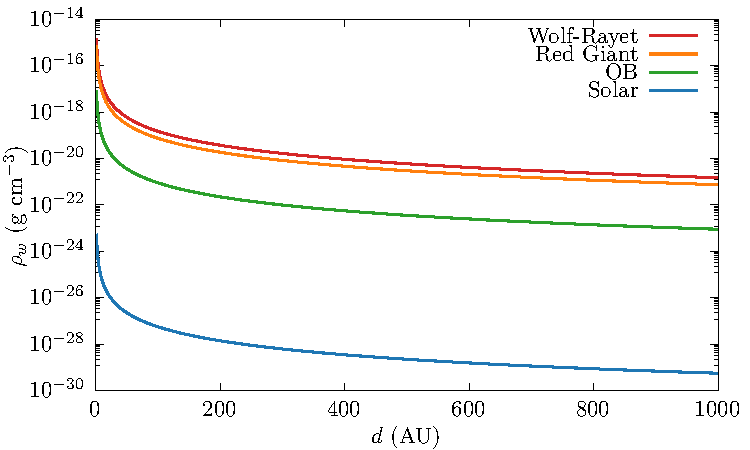
\includegraphics{assets/wind-comparison/wind-comp.pdf}
  \caption[$\rho_w$ comparison of main sequence winds]{Comparison of the densities of various main sequence winds using the parameters specified in table \ref{tab:windcomp}, wind densities are estimated using the smooth wind approximation described in equation \ref{eq:smoothwind}.}
  \label{fig:windrhocomp}
\end{figure}

\subsection{The CAK formalism}
\label{sec:cak}

\section{Interstellar Dust}
\label{sec:dust}

\subsection{The importance of interstellar dust}
\label{sec:dustimportance}

\subsection{Interstellar dust in massive star systems}
\label{sec:dustmassivestars}

\subsection{Radiation processes in interstellar dust}
\label{sec:dustcooling-background}

\section{Colliding Wind Binary Systems}
\label{sec:cwb}

% Introduction 


% //TODO Cannot get into the groove of this paragraph, please fix this future Joe
Colliding Wind Binaries\footnote{Abbreviated to CWBs.}, in opposition to all known laws of astrophysical nomenclature, is a easy to understand term - it is a binary system where stellar winds from the member stars undergoing collision.
Unfortunately, the simplicity of the systems ends here, CWB systems are extremely complex and poorly understood as they are difficult environments to observe or simulate.

%History and classification, useful sources in Stevens & Pollock 1994 

Early observations beyond visual spectrum led to the discovery of many new astrophysical phenomena, one such discovery were extremely bright persistent thermal x-ray sources, with x-ray 
The first classification and analysis of Colliding Wind Binary systems were independently performed by \textcite{prilutskii_x_1976} and \textcite{cherepashchukDetectabilityWolfRayetBinaries1976}, these systems were found to contain a close binary system, consisting of an evolved WR star and an OB counterpart, as their winds collide, a strong shock forms, heating the winds to temperatures in the order of $10^8$ \si{\kelvin} in the immediate post-shock environment, these extreme temperatures and the large quantity of shocked material accounted for the extremely bright thermal x-ray emission. The evidence was further compounded as the variation of the x-ray flux could be attributed to orbital motion of these binary systems.

% Early work categorising, using gamma 2 vel and V444Cyg

% Analysis pollock 1987 determined binary systems\cite{pollockEinsteinViewWolfRayet1987} 

% Formation 


\subsection{The Wind Collision Region}
\label{sec:wcr}

% What is this region
The Wind Collision Region\footnote{WCR} is the most violent and turbulent region of a CWB system, a region where strong shocks lead to temperatures in excess of $10^8$ $\si{\kelvin}$.
These strong shocks contain enormous amounts of mechanical energy, in the region of $10^3$ $\si{\solarluminosity}$, WCRs are engines capable of producing huge quantities radiation through multiple thermal and non-thermal mechanisms \parencite{eichler_particle_1993,grimaldoProtonAccelerationColliding2019}.
Despite these extreme conditions, these regions are capable of producing amorphous carbon dust grains at a rate on the order \num{1e-8} \si{\solarmass\per\year}.
As these grains are extremely fragile, this is a conundrum that has plagued researchers in this field, as direct observation of the innermost regions of even nearby WCRs is difficult, bordering on impossible, much of the work in this area involves hydrodynamical simulation.

% Properties of region

%//TODO This needs a lot of work, writing equation sections is boring

% Equations
The properties of the WCR can be described by a small number of parameters.
The first of such parameters is the wind momentum ratio, $\eta$, which describes the available \parencite{usov_stellar_1991}.


\begin{equation}
  \eta = \frac{\dot M_\text{OB} v_\infty^\text{OB}}{\dot M_\text{WR} v_\infty^\text{WR}},
\end{equation}

%Theres a particular paper on improved analytical observations 

This momentum ratio can also be used to estimate the distance of the apex of the WCR to each star, using the following equations:

\begin{equation}
  r_\text{WR} = \frac{1}{1+\eta^{1/2}} , ~~~ r_\text{OB} = \frac{\eta^{1/2}}{1+\eta^{1/2}},
\end{equation}

where $r_{WR}$ is the distance from the WR star to the WCR apex, and $r_\text{OB}$ is the distance from the OB star to the WCR apex.
Work by \cite{eichler_particle_1993} goes further to utilise the momentum ratio to approximate the shape of the wind collision region, further out from the apex of the WCR, the region forms an approximately conical shape with an opening angle, $\theta_c$ of:

\begin{equation}
  \theta_c \simeq 2.1 \left(1 - \frac{\eta^{2/5}}{4}\right) \eta^{-1/3}, ~~ \text{for } 10^{-4} \leq \eta \leq 1, \label{eq:conic}
\end{equation}


% Considerations due to stagnation point flow \cite{stevens_stagnation-point_1994}

% Brief notes on astrophysical shocks, link to appendix

%Detailed breakdown of Wind collision region

\subsection{Cooling in the WCR}
\label{sec:wcrcooling}
%//TODO clean up this caption
%//TODO remove grid from plot
\begin{figure}[h]
  \centering
  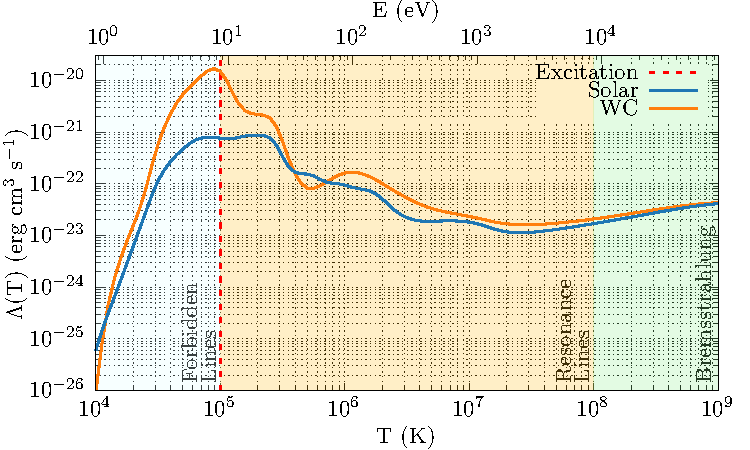
\includegraphics{assets/cooling-breakdown/cooling-curve-solar-withev.pdf}
  \caption[WC \& solar abundance plasma cooling curves]{Normalised plasma cooling rates as a function of temperature and thermal energy for solar abundance and WC abundance winds. The regions where forbidden line, resonance line and bremsstrahlung emission are dominant are highlighted, with H ionisation and recombination occuring between the forbidden and resonance line sections at $10^5$ \si{\kelvin}.}
  \label{fig:wcsolcooling}
\end{figure}

\begin{table}[h]
  \centering
  \begin{tabular}{lll}
  \\ \hline 
  \textbf{Temperature range} & \textbf{Dominant process} & \textbf{Spectral region} \\ \hline
  $\SI{5e3}{\kelvin} \lesssim T \lesssim \SI{1e5}{\kelvin} $ & Forbidden lines & IR, Optical \\
  $T \approx \SI{1e5}{\kelvin}$ & H excitation/ionisation & Optical, UV \\
  $\SI{5e3}{\kelvin} \lesssim T \lesssim \SI{1e5}{\kelvin} $ & Resonance lines & Far UV, soft X-ray \\
  $T \gtrsim \SI{1e8}{\kelvin} $ & Bremsstrahlung & Radio \\ \hline
  \end{tabular}
  \caption[Cooling processes at various temperature ranges]{Breakdown of dominant cooling processes at various temperature ranges from \cite{dysonPhysicsInterstellarMedium2021}, whilst H excitation/ionisation occurs over a very short temperature range, it is extremely influential, causing a global peak in the cooling rate at $\approx 10^5$ \si{\kelvin}. These temperature ranges are depicted in figure \ref{fig:wcsolcooling}.}
  \label{tab:coolprocess}
  \end{table}

% Radiative cooling, include graphs, mechanisms

Cooling due to radiation emission in a hot plasma can be broken down into a variety of processes that occur over series of temperature ranges.
Ions inside a plasma can become excited through collisions or photon absorption resulting in emission of photons as the ions de-excited. 

Mechanisms that are significant within the warm\footnote{See what I mean about the phrase ``warm''?} and hot gas phases include forbidden line emission, hydrogen excitation and ionisation, resonance lines and bremsstrahlung \parencite{dysonPhysicsInterstellarMedium2021}.
The influence of each mechanism waxes and wanes as temperature increases, with each mechanism dominant over a certain temperature range (table \ref{tab:coolprocess}).

% Section on forbidden line emission

The first mechanism to be discussed is forbidden line emission\footnote{Like many other phenomena discussed in this thesis, this too is a misnomer, while initially assumed to be prohibited under the contemporary understanding of atomic physics, it is in fact just astrophysicists jumping the gun again.}.
This process dominates the cooling process of cooler gas that is not fully ionised, where collisions with free electrons excite metals within the gas, causing them to de-excite through photon emission through these forbidden lines.
Forbidden lines themselves arise from magnetic dipole and quadrupole fine structure states within typical energy levels, despite having a much lower probability of occurring compared to conventional energy level transitions.
This process dominates at these temperatures as the transition energies are significantly lower, on the order of 1 \si{\electronvolt}, as the photon is also of a comparatively long wavelength, it can more easily escape from the gas without being re-absorbed by it.

% Section on ionisation/recombination

As the temperature increases there is a spike in the cooling rate of the gas as the hydrogen present begins to fully ionise, at this temperature a hydrogen ion and an electron may recombine, releasing a cascade of photons as the electron de-excites.

% Section on resonance line emission

As the plasma heats further resonance lines can

% Section on braking radiation

As the particle energy reaches the range of tens of \si{\kilo\electronvolt}, bremsstrahlung\footnote{Or braking radiation when you can't remember how to spell it.} becomes dominant (figure \ref{fig:wcsolcooling}). High velocity electrons are deflected by ions, emitting radiation in the process due to conservation of energy. 

% \parencite{1993ApJS...88..253S}
\parencite{schureNewRadiativeCooling2009}
\parencite{rybickiRadiativeProcessesAstrophysics2004}




%//TODO clean up this caption
%//FIXME use the new cooling code for this graph, early changes in ionisation fraction result in a different appearance from 1e4 to 1e6 kelvin!
\begin{figure}
  \centering
  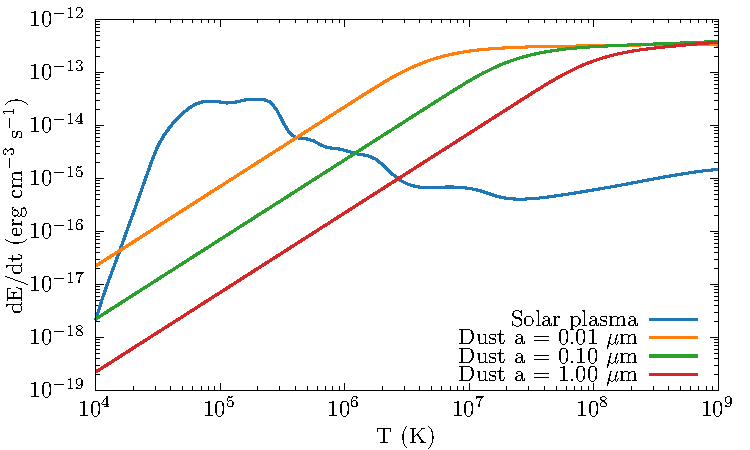
\includegraphics{assets/dust-plasma-cooling-comparison/cooling-comparison.pdf}
  \caption[Dust cooling vs. plasma cooling]{Comparison of plasma cooling to dust cooling with different grain sizes in a solar abundance gas, where $\rho_g = 10^{-20}$ \si{\gram\per\centi\metre\cubed} and a dust-to-gas mass ratio of 0.01.}
  \label{fig:dustplasmacomparison}
\end{figure}

% Needs to be spun off into a subsection

% Cooling parameter

\begin{subequations}
  \begin{align}
    \tau_\text{cool} & = \frac{k_B T_s}{4n_w \Lambda(T_s)} \label{eq:taucool} ,\\ 
    \tau_\text{esc}  & = \frac{d_\text{sep}}{c_s} \label{eq:tauesc} ,
  \end{align}
\end{subequations}

\begin{equation}
  \chi = \frac{\tau_\text{cool}}{\tau_\text{esc}} \approx \frac{v^4_{\infty,8} d_\text{sep,12}}{\dot M_{-7}} \label{eq:coolingparameter} ,
\end{equation}

% Dust cooling? Might need to move CWB dust formation up
The presence of dust within the immediate post-shock environment significantly increases the cooling rate.
Figure \ref{fig:dustplasmacomparison} compares rate of cooling due to dust emission of various types of grains to plasma cooling at solar abundances, 
As $\Lambda_g$ and $\Lambda_D$ are both proportional to $\rho_g^2$, dust cooling will dominate at high temperatures so long as there is sufficient amounts of dust.
%//TODO Lengthen paragraph, introduction to dust cooling

As dust grains collide with ionised gas and electrons, this imparts kinetic energy into the grains, heating them and causing them to emit infrared radiation. Assuming that there is a net accretion of ions and electrons onto the dust grains and the gas is optically thin in the infrared regime, energy is efficiently removed from the gas.
At particularly high temperatures this effect can dominate over high-temperature plasma cooling processes such as bremsstrahlung, as seen in figure \ref{fig:dustplasmacomparison}.
Figure \ref{fig:collisionalheatingcomparison} compares dust grain heating rates due to electron and ion collisional excitation in a solar abundance and WC abundance flow.
At lower temperatures the dust grain cooling rate is dominated by electron excitation, especially in the WC case as the ratio of free electrons to ions is significantly higher, as the WC flow is enriched by heavier elements.
However, as the grain temperature increases, collisional heating due to ions becomes more prevalent as the electrons are sufficiently energetic to pass through the grain without significant energy transfer; this is referred to as the electron transparency, $h_e$ \parencite{dwek_infrared_1981}.

\begin{figure}[h]
  \centering
  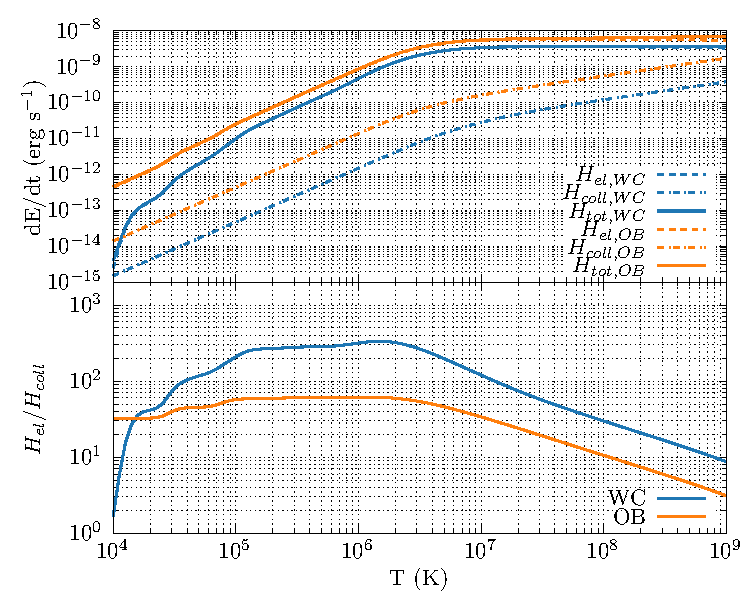
\includegraphics{assets/dust-electron-contribution/coll-el-comp.pdf}
  \caption[$H_{el}$ and $H_{coll}$ comparison]{Comparison of grain heating rate due to ion collisional excitation, $H_{coll}$, and electron excitation, $H_{el}$. The dust grain has a grain radius of \SI{5e-3}{\micro\metre} and is travelling through a gas with a density of $10^{-20}$ \si{\gram\per\centi\metre\cubed} with solar and WC abundances.}
  \label{fig:collisionalheatingcomparison}
\end{figure}


Work by \cite{dwek_infrared_1981} is used predominantly in this project to simulate cooling due to dust, a fast method for calculating the cooling rate due to dust was integrated into the numerical code for this project, which is elaborated on in section \ref{sec:dustcoolingmodel}.
% Finish and link to below paragraph

%Find citation for spitzer 1978

The heating rate of a dust grain due to collisions 

\begin{equation}
  \begin{split} 
      H_\text{coll} = & n \pi a^2 \langle Q(E,q,U) \rangle \\
      & \times \langle v (E-qU) f(a,E-qU) f(a,E-qU) \rangle \, \si{\erg\per\second}
  \end{split}
\end{equation}

%Explain constants
This can be simplified and expressed in the equation:

\begin{equation}
  \begin{split}
    H_\text{coll} & = \left(\frac{32}{\pi m}\right)^{1/2} n\pi a^2 (k_B T)^{3/2} h(a,T) \\
    & = \num{1.26e-19} \frac{n}{A^{1/2}} a^2 (\si{\micro\metre}) T^{3/2} h(a,T) \, \si{\erg\per\second}
  \end{split}
\end{equation}

% This part is very dry and is going to explain the equations more in depth
% Main source will be dwek 1981 appendix 2



% Instabilities due to cooling, might spin off into it's own appendix chapter?
% Theres a particular paper that covers this 
% Mainly need to discuss KH instabilities, and how they relate to cooling



\subsection{Dust formation in CWB systems}
\label{sec:cwbdust}

%Intro to dust formation in said systems
Despite the extremely violent conditions thus far described in CWB systems, these systems appear to be extremely prolific producers of interstellar dust.
Whilst single star WC systems can produce small amounts of dust in the form of amorphous carbon grains (though this could be observed to be extremely rare, pending the results of \textcite{medinaAreAllWCd2021}), binary systems have been observed to convert up to $10^{-3}$ of their wind masses from ionised carbon into amorphous carbon dust grains, this results in a typical dust production rate of $10^{-8} \, \si{\solarmass\per\year}$, on part with a typical Asymptotic Giant Branch (AGB) star.
This dust forming behaviour has only been observed in particularly energetic WC stars (predominantly WC9, with some WC7-8 examples), WN and WO systems have not been observed producing dust, this is most likely due to amorphous grains being significantly more chemically stable and resilient to effects such as sublimation and photoevaporation than water ice or silicate grains \parencite{salpeter_formation_1977,draineDestructionMechanismsInterstellar1979}.
Dust formation is also observed to form within the WCR, which can form quite beautiful pinwheel-shaped patterns, as dust streams away from the stars in the post-shock outflow.

\begin{table}[]
  \centering
  \begin{tabular}{ccccccc}
    & \multicolumn{2}{c}{Persistent} & \multicolumn{2}{c}{Variable} & \multicolumn{2}{c}{Episodic} \\ \cline{2-7} 
    & Total & Example & Total & Example & Total & Example \\ \hline
   WC4 & 1 & WR19 & 0 & --- & 0 & --- \\
   WC5 & 0 & --- & 0 & --- & 1 & WR47C \\
   WC6 & 1 & WR124-10 & 0 & --- & 0 & --- \\
   WC7 & 3 & WR102-22 & 0 & --- & 4 & WR140 \\
   WC8 & 6 & WR13 & 1 & WR48a & 3 & WR122-14 \\
   WC9 & 45 & WR104 & 6 & WR98a & 1 & WR75-11 \\ \hline
   Total & 56 &  & 7 &  & 9 &  \\ \hline
  \end{tabular}
  \caption[Numer of confirmed WCd systems]{Number of confirmed WCd systems with known spectral type and dust formation type from the Galactic Wolf Rayet Catalogue \parencite{rossloweSpatialDistributionGalactic2015}, systems with uncertain spectral types not included, while systems labelled ``d'' are included within the ``persistent'' category for their associated spectral type.}
  \label{tab:wc-summated-list}
\end{table}

% Rarity
Whilst beautiful, they are sadly an elusively rare beauty...
The Galactic Wolf Rayet Catalogue\footnote{The most recent version of this catalogue is available at \texttt{\href{http://pacrowther.staff.shef.ac.uk/WRcat}{http://pacrowther.staff.shef.ac.uk/WRcat}}} \parencite{rossloweSpatialDistributionGalactic2015} has a collection of 667\footnote{At time of time of writing, with the last update being August 2020.} known galactic WR stars, 106 of such stars are contained within a binary system, with 41 such binaries containing WC stars.
\textcite{rossloweSpatialDistributionGalactic2015} notes that there are a total of 42 confirmed WCd systems, approximately 35\% of all WC systems, though this value is somewhat out out date and includes single star systems.
A more up-to-date estimate performed for this thesis using the updated dataset estimates a total of 80 WCd systems, of which 72 have well-determined spectral subtypes (table \ref{tab:wc-summated-list}).
% Impact of systems 
\textcite{rossloweSpatialDistributionGalactic2015} goes on to estimate that out of an estimated total of 1900 galactic WR stars, approximately 300 of these stars are predicted to be dusty WC stars.
Whilst this is a far cry from the number of galactic AGB stars - of which carbon-rich AGBs outnumber WCd stars by approximately 3 orders of magnitude \parencite{ishiharaGalacticDistributionsCarbon2011} - these systems can still significantly impact the surrounding interstellar medium, with strong stellar feedback propagating large quantities of dust into the surrounding medium.

% Number of WCd systems, reasoning for only certain subtypes being dust forming
Table \ref{tab:wc-summated-list} contains an excerpt of the observed WCd systems with clearly defined spectral subtypes, most dust producing stars are either WC8 or WC9 subtypes, which are markedly cooler and less luminous than their WC4 counterparts.
This reduced luminosity is potentially the driving factor for dust formation in the system.
As WC8-9 systems have slower, cooler winds \parencite{niedzielskiKinematicalStructureWolfRayet2002}, they are more strongly influenced by post-shock cooling, allowing for greater dust formation within the WCR.
A small number of these systems have somewhat variable or episodic dust production cycles, such as WR98a and WR140, which are the two systems being observed within this thesis.
Furthermore, the bulk of WCd systems do appear to be in binary systems with a close periastron passage, in fact, this orbit itself appears to be a driving force behind how dust is produced in these systems, as we will later discuss.

%Theories as to why
A good starting point to understanding dust formation is to understand how the WCR can mitigate the mechanisms resulting in dust destruction, whilst aiding the processes involved in dust formation.
As previously discussed, dust can be destroyed through high-velocity collisions with grains, as well as evaporation through heating or ionising radiation.
These processes are mitigated through the cooling, as well as the high level of UV extinction due to the high density of the WCR.
Meanwhile, the dust production rate increases within high density regions, as collisions between dust grains and gas occur at a much higher rate.
The same can be said with dust grains, allowing for fast growth from gas and impinging ion accretion, and grain-grain collision as the number density of dust grains begins to increase.
The accumulation of these effects would be a very fast initial growth rate, which tapers off as the post-shock region diffuses and expands, resulting in a reduction in density.

% Role of instabilities
The presence of instabilities driven by cooling and other factors can lead to pockets of high density post-shock material, as high density drives dust formation, this can lead to ``clumps'' of highly dust-enriched post-shock stellar wind.
These clumps would have additional protection from UV photons, and would also be cooled enough for dust to form, thus, the driving hypothesis for this theory is that these are regions where the bulk of dust formation would occur.
% How to make lots of dust + reminder of aims of project.
As such, it is theorised in order to achieve a high rate of dust formation, a dense, highly radiative post-shock WCR must be formed, as cooling in the post-shock region is dependent on separation distance, wind velocity and mass loss rate, these parameters should first be explored, with the knowledge gleaned used to direct an analysis of observed systems such as WR140.

%Observational data Link to Crowther papers in particular, dust formations only around WC
% Discuss role of eccentricity
Eccentricity appears to play an important factor in the production of dust, highly eccentric systems can vary their dust production rates significantly.
Figure \ref{fig:periodicmags} shows the periodic change in mid-IR emission that can be explained as dust emission from small amorphous carbon grains, in the case of systems such as WR140 or WR125 dust production can be reduced to the point where associated emissions can drop by several magnitudes.
This relation is clearly periodic, with a peak in dust production production coinciding with the periastron passage of these systems.
This implies that dust production is dependent on orbital separation, which will influence the degree of cooling occurring within the WCR, it could potentially also alter the wind velocity on collision, which will also influence dust production in the same manner.
% Metastudy
Further analysis of available dust producing CWB systems suggests that \textit{all} WCd systems with circular orbits produce dust either persistently or with a degree of variability, while eccentric WCd systems are solely produce dust episodically.

\begin{figure}
  \centering
  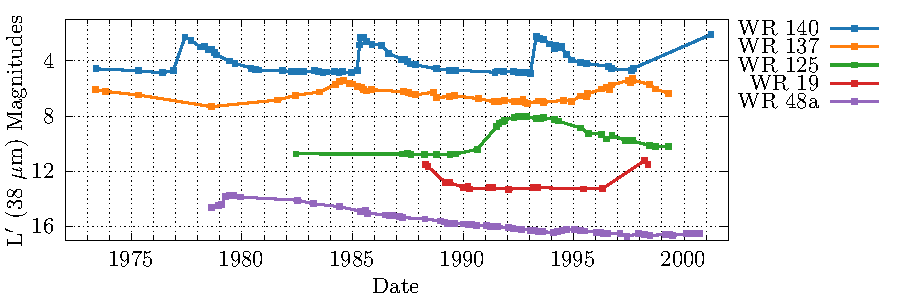
\includegraphics[]{assets/magnitudes/magnitudes.pdf}
  \caption[L$^\prime$ photometry of episodic dust making stars]{L$^\prime$ photometry for episodic dust making stars, data derived from \textcite{crowther_dust_2003}, and provided by PM Williams in private correspondence. WR 140 and WR 137 in particular have extremely predictable dust forming events which correspond to periastron passage in both systems.}
  \label{fig:periodicmags}
\end{figure}


\subsection{Important WCd systems}

The principle systems that are being observed in this thesis are the variable dust forming system, WR98a, and the episodic dust forming system WR140.
The archetypal continuous dust forming system WR104 was also proposed for simulation, but had to be cut due to time constraints, this system will also be discussed to provide a point of comparison between the two systems.

\begin{table}[h]
  \centering
  \begin{tabular}{cccccccc}
  \hline
  System & $\dot{\text M}_{\text{WR}}$ & $\dot{\text M}_{\text{OB}}$ & $v_{\text{WR}}^\infty$ & $v_{\text{OB}}^\infty$ & $\eta$ & $\chi_\text{min}$ & $\dot{\text M}_\text{D}$ \\
   & (\si{\solarmass\per\year}) & (\si{\solarmass\per\year}) & (\si{\km\per\second}) & (\si{\km\per\second}) & (AU) & & (\si{\solarmass\per\year}) \\ \hline
  WR98a & \num{5.0e-6} & \num{5.0e-8} & 900  & 2000 & 0.0222 & 0.7970 & $\left(6.10^{+1.77}_{-1.38}\right) \times 10^{-7}$ \\ 
  WR104 & \num{3.0e-5} & \num{6.0e-8} & 1220 & 2000 & 0.0033 & 0.2430 & $\left(4.39^{+1.27}_{-0.97}\right) \times 10^{-6}$ \\
  WR140 & \num{5.6e-5} & \num{1.6e-6} & 2895 & 3200 & 0.0314 & 2.6866 & $\left(8.11^{+4.83}_{-4.15}\right) \times 10^{-10}$ \\ \hline
  \end{tabular}
  \caption[Wind properties of systems considered for simulation]{Wind properties of systems considered for simulation in this thesis.}
  \label{tab:systems-wind-properties}
\end{table}

\begin{table}[h]
  \centering
  \begin{tabular}{ccccccc}
  \hline
  System & Period & Eccentricity & $M_{\text{WR}}$ & $M_{\text{OB}}$ & Periastron & Apastron \\
   & (d) & ($e$) & (\si{\solarmass}) & (\si{\solarmass}) & (AU) & (AU) \\ \hline
  WR98a & 556 & $\sim 0$ & 10.0 & 18.0 & 4.06 & 4.06 \\
  WR104 & 245 & 0.0600 & 10.0 & 20.0 & 2.20 & 2.48 \\
  WR140 & 2869 & 0.8993 & 10.31 & 29.27 & 1.53 & 26.9 \\ \hline
  \end{tabular}
  \caption[Orbital properties of systems considered for simulation]{Orbital properties of systems considered for simulation in this thesis.}
  \label{tab:systems-orbital-properties}
\end{table}

\subsubsection{WR98a}

\begin{figure}
  \centering
  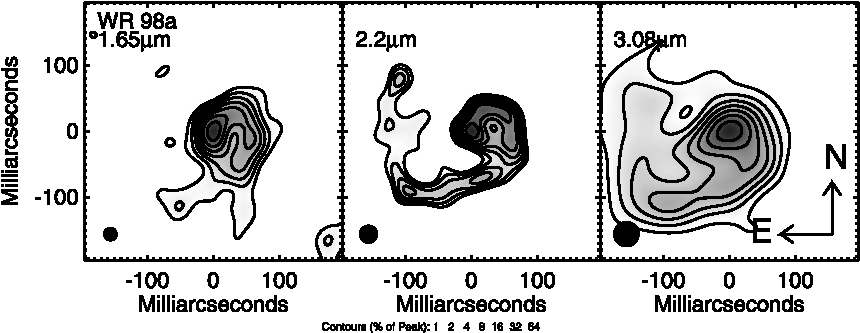
\includegraphics{assets/systems/wr98a-monnier2007.pdf}
  \caption[\textit{Multiwavelength image of WR98a \parencite{monnierKeckAperturemaskingExperiment2007}}]{Multiwavelength aperture synthesis images of WR98a taken on June \nth{24} 2000, at 1.65, 2.2, and \SI{3.08}{\micro\metre}. Plot sourced from \textcite{monnierKeckAperturemaskingExperiment2007}, the significant IR excess is a clear sign of ongoing dust production. The system also has a pronounced pinwheel structure most prominent at \SI{2.2}{\micro\metre}.}
\end{figure}

% Physical properties

WR98a is a  

% Historical observation 

% Hendrix paper dust formation monnier 2002 radio domain

% Questions as to orbit shape, approximately circular

% Ease of simulation, good starting point

% Parameter space exploration
Because of this relative ease of simulation and relatively slow wind velocity for both stars in the system, WR98a was chosen to be the baseline system for the research conducted in chapter \ref{chap:parameterspace}.

\subsubsection{WR140}

% Physical properties

% Historical observation
WR140 is significant in that it is the first system to be observed with episodic dust forming CWB properties, \textcite{williamsCondensationShellHD1978} notes a rapid brightening in the infrared, suggesting the formation of a new shell of dust around the system.
WR140 has undergone frequent observations, with spectroscopic data going back to 1972, and is perhaps the most well-observed episodic WCd system, for this it was immediately considered for 

% Eccentric orbit, variable dust formation

% Difficulty of simulation
As it is a highly eccentric system with a particularly long period orbit, a number of difficulties 

with the constraints of only having SMR available throughout this project, with AMR not currently being stable in this particular hydrodynamical code, 
% Snippet
As such, it was decided to only simulate the system as it undergoes closest approach, from $\phi = 0.95$ to $\phi = 1.10$, as a full orbit of the system would require AMR to undertake within the time constraints remaining in this project. 


\subsubsection{WR104}

\begin{figure}
  \centering
  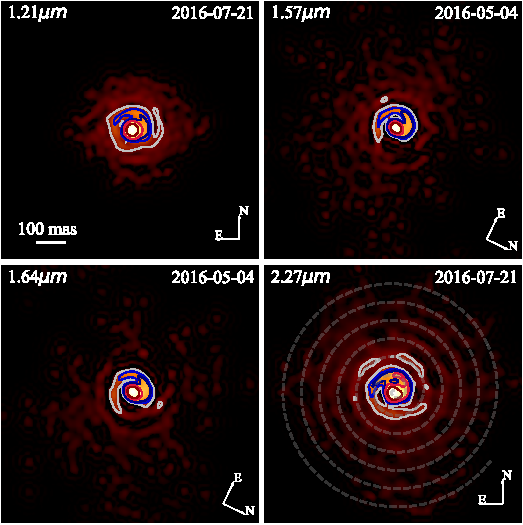
\includegraphics[]{assets/systems/soulain-2018-wr104.pdf}
  \caption[\textit{Spiral structure of WR104 \parencite{soulainSPHEREViewWolfRayet2018}}]{Deconvolution of J, H, K, and \SI{2.27}{\micro\metre} bands of WR104 sourced from \textcite{soulainSPHEREViewWolfRayet2018}. The spiral pattern and first revolution is visible in all images, in particular at \SI{2.27}{\micro\metre}.}
  \label{fig:soulain-wr104}
\end{figure}

% Physical properties
WR104 is an archetypal example of a continuous WCd system, it is a comparatively tight binary with a semi-major axis of \SI{2.34}{\au} and a period of $\sim 241$ days, the orbit is also relatively circular, with an eccentricity of $e = 0.06$ \parencite{lamberts_colliding_2012}.
The system consists of a WC9 star with a B0.5V partner \parencite{williamsSpectroscopyWC9WolfRayet2000}, this combination of a WC star and a comparatively weak B partner results in a severely imbalanced wind, with a momentum ratio of $0.003$, an order of magnitude lower than WR98a.
This imbalanced wind, combined with the tight orbit, results in an extremely strong WCR that is constantly churning out dust.
% Mass loss rate
Using radiative transfer models, \textcite{harries_three-dimensional_2004} calculated a dust production rate of \SI{8(1)e-7}{\solarmass\per\year}, corresponding to 2\% of the carbon mass loss rate of 
A more advanced model by \textcite{lauRevisitingImpactDust2020}, which is used to assess the dust formation rates of systems in this thesis, calculated the dust formation rate to be $\left(4.39^{+1.27}_{-0.97}\right) \times 10^{-6}\, \si{\solarmass\per\year}$.

% Why is it archetypal 

WR104 can be considered to be an ideal example of a continuous dust forming system, the system is relatively close, at a distance of \SI{2.5}{\kilo\parsec}, and is at an inclination that is almost face-on relative to Earth, at $i \lesssim 16^\circ$. 
As such, the pinwheel outflow from the system can be clearly resolved, with infrared excess due to dust clearly observed within the pinwheel structure (\textcite{soulainSPHEREViewWolfRayet2018}, see figure \ref{fig:soulain-wr104}).
Due to the systems parameters and well defined observable dusty pinwheel structure, along with prior observations and simulations of the system, it is an ideal candidate for simulation 

There are a number of reasons for this prodigious dust formation rate, as the systems orbit is comparatively close and circular with a very dense primary wind, the wind is expected to be highly radiative throughout the entire orbital period, this suggests a cool post-shock WCR that can continuously produce dust.
The estimated cooling parameter is more than an order of magnitude lower than the other systems considered for simulation, leading to a

% Why it wasn't assessed, difficulty of simulation, needed AMR
Unfortunately, despite being a very strong candidate for simulation, attempting to simulate the system proved to be exceptionally difficult.
% Many level simulation required for large-scale observation
The very close orbit of the system would mandate a very high simulation resolution, increasing the amount of compute time required to finish the simulation, only simulating a small region would prevent the pinwheel from being formed and observed, which we would have ideally wanted to include.
% Instability required running at very low Courant number
In addition the strong radiative cooling resulted in the simulation being very unstable unless the Courant number is exceedingly small, this also significantly increases compute time.
With a limited amount of compute resources as well as a limited amount of time, this stretched the feasibility of simulating this system.
% Physical effects, gayley
As the wind from the primary star is significantly stronger than its partners, WR104 has a much lower momentum ratio than the other systems being considered, as such, the WCR is situated much closer to the secondary star.
At closest approach, $r_\text{OB} \approx \SI{60}{\solarradius}$, which would require WR104 to be simulated at a much higher resolution, in turn demanding significantly more computational resources.
Physical effects, such as radiative inhibition and sudden braking may also significantly alter the wind velocity and post-shock environment, reducing the pre-shock primary wind velocity \textcite{gayley_sudden_1997}.
The pre-shock secondary wind velocity would also be influenced, due to insufficient acceleration from line driving before the winds collide.
As radiative line driving is not simulated these effects cannot be taken into account, and would have resulted in an inaccurate simulation of the system.
The effect of incomplete acceleration and sudden braking in highly wind-imbalanced systems is discussed more substantially in section \ref{sec:simassumptions}.
% Why it was discarded
With limited time remaining in the project, as well as the above factors, simulation work on WR104 was abandoned in favour of a parameter space search of a system with baseline properties similar to WR98a, as well as a limited simulation of WR140. 
Simulating this system however, is a particularly enticing avenue of future research.

\subsection{WR+WR systems}

Recently, two candidates of a theorised subset of CWB have been discovered - WR+WR systems, which have a \textit{second} Wolf-Rayet star as their partner, with a secondary wind around 3 orders of magnitude denser than a WR+OB system, this would of course result in a truly titanic wind collision.
These candidates are the recently discovered WR70-16 \parencite{callinghamAnisotropicWindsWolf2019}, and the previously discovered WR48a system \parencite{danksInfraredSpectroscopyInfrared1983}, which exhibits the spectroscopic lines of both a WC and WN system \parencite{williamsVariableDustEmission2019}.
These systems are predicted to be comparatively rare, even among CWB systems, this is largely due to unlikelihood that both stars in the system would be in their Wolf-Rayet phase at the same time.
Despite these systems having an enormous combined mass-loss rate, initial estimates of the dust production rates of both systems indicate that their dust conversion efficiencies are comparatively low compared to less energetic systems, and overall quite mundane dust production rates in general.
Whether this suppressed dust production rate is a common phenomena among WR+WR systems remains to be seen, as more systems would need to be discovered in order to determine this.

\subsubsection{WR70-16 (``Apep'') -- a recently discovered WR+WR system}

\begin{figure}
  \centering
  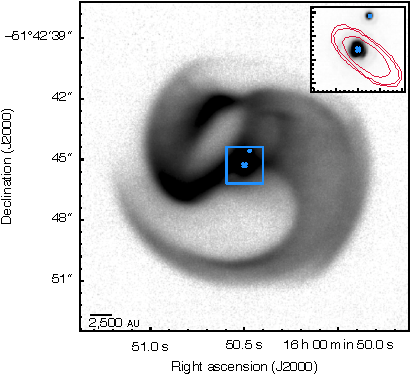
\includegraphics[]{assets/systems/apep-callingham-2019.pdf}
  \caption[\textit{VLT image of Apep \parencite{callinghamAnisotropicWindsWolf2019}}]{\textcite{callinghamAnisotropicWindsWolf2019}}
  \label{fig:apep-callingham}
\end{figure}

A potential avenue of research for this field is the simulation of WR+WR systems such as the recently discovered WR70-16 system (hereafter referred to as ``Apep''), this system was discovered due to the significant difference between the spectroscopically derived wind velocity of \SI{3400(200)}{\kilo\metre\per\second} and the observed expansion speed of \SI{570(70)}{\kilo\metre\per\second}  \parencite{callinghamAnisotropicWindsWolf2019}.
This inhibited wind velocity, far below any categorised WR wind velocity, suggests that much of the wind undergoes collision with the wind of a binary partner.
The extremely luminous non-thermal and infrared emission, suggested two extremely high mass loss rate stars within the system, as well as evidence for a third, distant partner in a loose trinary system \parencite{callinghamTwoWolfRayet2020}.
Spectroscopic analysis suggested that the central component of the Apep system consists of a nitrogen sequence WN4-6b and a carbon sequence WC8 star, with more more massive and luminous WN4-6b star kinematically dominating the system.
This discovery is very significant as it is the first galactic WR+WR system discovered, other systems have been identified, but are extragalactic in nature.

Further work by \textcite{hanExtremeCollidingwindSystem2020} has estimated the orbital parameters of Apep, finding that it is a highly eccentric system with a period of \SI{125(20)}{\year} and an eccentricity of \num{0.7(0.1)}, inclined at $\pm \ang{30} \pm \ang{5}$ towards Earth.
An initial estimate of the dust formation rate was made, finding a dust production rate of $\sim \SI{5e-7}{\solarmass\per\year}$, while observation of the surrounding dust shell suggests that it is a periodic dust forming system, which is sensible considering the systems high eccentricity.

The opening angle of the WCR was found to be very wide, at $\ang{125}\pm\ang{10}$, further suggesting the presence of two very high mass loss rate objects within the system, suggesting relatively balanced wind momenta for a CWB system.
Additional calculations by \textcite{marcoteAUscaleRadioImaging2021} estimated the systems wind momentum ratio to be $0.44\pm 0.08$, again in line with WR+WR hypothesis. 
Finally, pre-print work by \textcite{delpalacioNonthermalEmissionCollidingwind2021} finds a mass loss rate of \SI{4e-5}{\solarmass\per\year} for the WN star and \SI{2.9e-5}{\solarmass\per\year} for the WC star, which all but confirms the presence of a WR+WR binary at the heart of Apep.

With an estimated combined mass loss rate of \SI{6.9e-5}{\solarmass\per\year} we can estimate that the system has a dust conversion efficiency of 0.7\%;
whilst this system is therefore not a prodigious producer of dust this is most likely due to the extremely high wind terminal velocity and high separation distance, which would suggest a fairly smooth and adiabatic post-shock region. 
We can estimate the cooling parameter of the system to be $\sim 80$, based on angular separation from \textcite{hanExtremeCollidingwindSystem2020}, confirming that at present, the winds are adiabatic.
In order to estimate the closest approach of the system, and therefore the minimum cooling parameter an accurate measure of the stellar mass of both objects would need to be made, there is insufficient data for this at the time of writing.

\subsubsection{WR48a -- revisiting a WR+WR candidate}

% Why simulate it? And difficulties therein
WR+WR systems appear to be incredibly rare, with only a small number of extragalactic WN sequence examples in the LMC \parencite{shenarWolfRayetBinaries2019}, as well as an additional galactic WR+WR binary candidate, WR48a, \parencites(){zhekovMultiwavelengthViewDusty2014}{williamsVariableDustEmission2019}{zhekovChandraRevisitsWR2022}.
In the case of WR48a, its change in classification from a dust forming WC8 with an unknown partner to a WC8-WN8 is contemporaneous with the discovery and classification of Apep, though there is a distinct lack of recent observations of the system compared to the more recent WR+WR candidate.

\textcite{lauRevisitingImpactDust2020} calculated a dust formation rate for WR48a of $\left(8.46^{+3.48}_{-4.38}\right) \times 10^{-8} \, \si{\solarmass\per\year}$ with a dust conversion efficiency of $0.12\%$, markedly less than other systems with much less available material.
A future avenue of research would be to simulate these systems to understand why the dust formation rate is comparatively low, despite the readily available stellar material.
The main difficulty of simulating these systems is the lack of orbital parameters and accurate mass loss rates, as WR48a has insufficient data and Apep has only been recently discovered, there are currently too many unknown factors in order to build an adequate simulacrum of the systems\footnote{A lack of accurate orbital parameters is also an issue in devising simulations for more conventional WR+OB systems}.
Another difficulty is the large degree of orbital separation, high eccentricity and long orbital timescales required to simulate these systems.
The current limitations of the hydrodynamical code being used in this project render it difficult to simulate entire orbital passes of highly elliptical systems with long periods, if these issues are resolved in later versions of the hydro code however, this would present an interesting avenue of future research.

\chapter{Methodology \& Numerical Simulation}
\label{ch:numsim}

% Brief summation of computational work
Observational astrophysics is a curious field based on snapshots.
The universe can be thought of as a near-infinite number of laboratory experiments, that are viewed from the astronomer from a fixed perspective, through a very large telescope.
Most phenomena too, evolve over incredibly long timescales, it may in some cases take the entire lifetime of a researcher to collect enough information on a single system - in other cases, they may be long dead before their predictions can be validated.
Despite this, by observing many systems at once, we can overcome this limit, piecing together the properties and formation of phenomena from a thousand disparate snapshots in space and time.
This kind of ``natural parallelisation'' works, to a point, and where it doesn't numerical simulation can step in.
While a comparatively recent method of research, and only within the last two decades has computing hardware been up to the task of simulating 3D environments, numerical simulation is vital for gaining insight on regions that are hard to observe.
The WCR of a CWB system is extremely difficult to observe, and as such, we turn to simulation in order to understand the region better.
Unfortunately, it is also comparatively difficult to simulate as well, as we will discuss.

% Why is this it's own chapter?
As mentioned in the introduction to this thesis, theoretical astrophysics straddles two complex fields, astrophysics and computer science.
To this end, while we have discussed the underlying physics and physical phenomena of this project, we have so far neglected to cover the simulationist aspects of this work.
Some astrophysicists reading this thesis may be unfamiliar with the computational side of the work, and vice versa for computer scientists - as such it is best to describe both in detail.
Furthermore, discussing our methodology in its own section consolidates it and makes it easier for the reader to understand and replicate it.
% Breakdown of chapter, what this involves
This chapter primarily deals with detailing numerical simulations, in particular how they work and why they are being utilised, as well the development and implementation of a CWB model inside the \athena{} hydrodynamical code.
We also detail our attempts to implement radiative cooling, as well as our advected scalar dust model, \bidmas.

\section{The History \& Mathematics of Numerical Simulations}
\label{sec:numerical-math}
\label{sec:numsim}

% Numerical solvers/Riemann problems
In astrophysical fluid dynamics, the most fundamental of equations are the Euler equations.
These are a specific case of the more general Navier-Stokes equations of fluid dynamics, covering the case of an inviscid fluid lacking thermal conductivity.
These properties make the equations ideal for application to astrophysical fluids.
At vast length scales the aggregate properties of a collection of molecules in near vacuum are essentially in-line with what is predicted by inviscid fluid dynamical equations.
Because of the general lack of physical contact, being both rare and fleeting, the influence of thermal conduction and convection on the fluid are essentially ruled out.
Astrophysical fluids at first appear strange and unintuitive compared to the more familiar fluid dynamics that we have an almost innate understanding of as human beings.
However, if one zooms out enough and starts thinking in terms of parsecs and astronomical units, some similarities do appear, such as instabilities, turbulence and shocks.

In a one-dimensional adiabatic case, with a fluid of density $\rho$, a velocity of $u$, a fluid pressure of $P$ and a total energy, $E$, the Euler equations take the form:

\begin{subequations}
  \begin{align}
    \frac{\partial \rho}{\partial t} & + \frac{\partial}{\partial x} (\rho u) = 0 ,\\
    \frac{\partial \rho u}{\partial t} & + \frac{\partial}{\partial x} (\rho u^2 + P) = 0 ,\\
    \frac{\partial E}{\partial t} & + \frac{\partial}{\partial x} \left[ u(E+P) \right] = 0 .
  \end{align}
\end{subequations}

\noindent
As the Euler equations are a non-linear series of partial differential equations, no general analytical solution exists, to make it worse, numerical solutions aren't exactly easy either.
% Godunov method and other exact methods
The basest method of numerically solving such problems is Godunov's scheme \parencite{godunov_difference_1959}; this scheme is a finite-volume method wherein the problem is split into a series of cells, with a Riemann problem between the interfaces of each cell (Fig. \ref{fig:riemann}), an approximate solution to the Euler equations can then be made by solving all of these Riemann problems in sequence and integrating across a time-step, $dt$.
The problem can be simulated and solved by marching through many time-steps, until the required advection time is achieved.
This provides a first-order accurate approximation in a more general form, compared to the otherwise intractable set of PDEs. 
Whilst this piecewise method of solving many thousands of Riemann problems may provide a more generalised method of calculating fluid dynamics, performing it by hand would invoke a terrible strain on a mathematician's wrists.

\begin{figure}[ht]
  \centering
  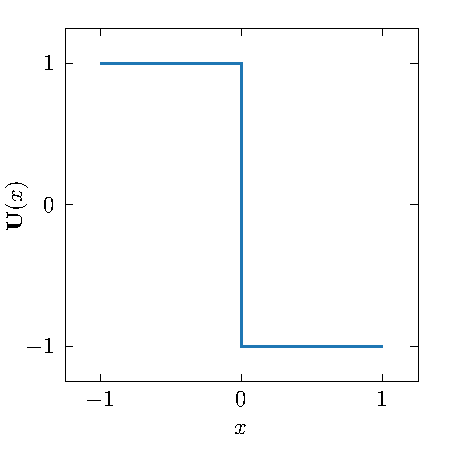
\includegraphics[]{assets/riemann-interface/riemann.pdf}
  \caption[Initial conditions of a Riemann problem]{The initial conditions of a Riemann problem, where $\mathbf{U}$ is a conserved variable.}
  \label{fig:riemann}
\end{figure}

Godunov's scheme however, coincided with the burgeoning field of computer science.
Computers are extremely well suited to this type of calculation, and can solve Riemann problems many orders of magnitude faster than a mathematician with repetitive strain injury.
Solving a higher-dimensional problem is a conceptually trivial extension to the original 1-D problem.
In the 2-D case the number of interfaces increases to 4, with each interface being the analogous to each side of a square or rectangle, while in the 3-D case the interfaces can be thought of as the 6 faces of a cuboid.
As such, the general formulation of the Euler equations becomes:

\begin{equation}
  \frac{\partial \mathbf{U}}{\partial t} + \nabla \cdot \left[ \mathbf{F}(\mathbf{U}) \right] = 0 ,
\end{equation}

\noindent
where $\mathbf{U}$ is a vector of conserved variables and $\mathbf{F}(\mathbf{U})$ is a vector of the corresponding fluxes of the conserved variables:

\begin{equation}
  \mathbf{U} = 
  \begin{bmatrix}
    \rho \\
    \rho u \\
    E
  \end{bmatrix}
  , ~
  \mathbf{F}(\mathbf{U}) =
  \begin{bmatrix}
    \rho \boldsymbol{u} \\
    \rho u \boldsymbol{u} + P \\
    \boldsymbol{u}(E + P)
  \end{bmatrix} .
\end{equation}

In practise however, solving higher-dimensional problems are significantly more computationally intensive, due to the increased number of interfaces and the drastically increased number of cells required to simulate the problem.

% HLLC method, as used in project

Initial methods involved exact solutions to the Riemann problems, however, this is a time consuming method.
Instead, approximate methods were developed to improve numerical performance.
However, early methods were less exact, and could not preserve the contact surface, these methods were also markedly less stable, limiting their effectiveness.
Later models, such as the Harten-Lax-van Leer-Contact (HLLC) solver \parencite{toroRestorationContactSurface1994} are approximate solvers that offer a similar order of accuracy to the exact solution, while being significantly faster than the exact solution and more numerically stable than earlier approximate solvers.
As such, this method is commonly used in hydrodynamical codes, and is used in this project as one of the methods included in \athena.

% Piecewise methods
Godunov's method is commonly used as a base for higher-order extensions, which employ methods to interpolate and reconstruct the flow between the interfaces of each Riemann problem.
Piecewise linear linearly interpolates fluxes between cells to reconstruct the cell interfaces, and is generally considered to be significantly more versatile than a simple piecewise \parencite{vanleerUltimateConservativeDifference1979}
The piecewise parabolic method performs a parabolic interpolation step instead, this is generally more accurate for a smooth and continuous flow, but most schema must account for and detect discontinuities
\parencite{colella_piecewise_1984}.
Throughout this project we use the piecewise linear method, which is the default for \athena{} and \mg{}.
This was found to be more than suitable for our work.

% Integration
In order to solve the problem, the fluxes along each cell interface are integrated across time, in the case of this project, a third-order accurate Runge-Kutta (RK) method is used.
% Courant number
The integration timestep is typically much smaller than the 
Overall, with $n$ spatial dimensions and 1 time dimension, it is clear how computationally intensive these simulations are.
This timestep must be carefully calibrated to ensure that the duration of the integration step is less than the time taken for a fluid to advect through to an adjacent cell.
If a clump of gas, for instance, travels across two adjacent cells in a single timestep, the interaction occurring in the middle cell would be lost, and unphysical behaviour would occur.
This is especially a problem in the case of highly supersonic flows, where the fluid is moving extremely fast.
This problem is further compounded with multiple dimensions, which must all be accounted for in a similar manner.
The Courant-Friedrichs-Lewy condition determines that the maximum integration time should not be higher than the time taken for a fluid to advect between adjacent cells in a numerical grid.
This condition defines a value $C$, or the CFL number, and is the ratio between the wave propagation speed, $u$, and the grid speed, $\Delta x / \Delta t$.
For multiple dimensions, the CFL number is calculated with the formulae

\begin{equation}
  C = \Delta t \left(\sum^n_{i=1} \frac{u_{x_i}}{\Delta x_i}\right) ,
\end{equation}

\noindent
where $\Delta t$ is the timestep, $u_{x_i}$ is the velocity of the fluid along dimension $i$ and $\Delta x_i$ is the cell spacing for dimension $i$ \parencite[Ch.~5]{toro_riemann_2013}.
Hydrodynamical codes typically allow the user to define $C$ such that the code can calculate the necessary timestep.
For instance, in the case of a three-dimensional problem, $\Delta t$ is found to be

\begin{equation}
  \Delta t = \frac{C}{(u_x/\Delta x) + (u_y/\Delta y) + (u_z/\Delta z)}.
\end{equation}

\noindent
For an explicit time-integration problem such as numerical simulation, the value of $C$ is typically $\leq 1$, with the timestep decreasing with additional dimensions for a given value of $C$.
For 3-dimensional problems in this work, we typically start at $C = 0.15$, and decrease if necessary.

\section{The Purpose of Numerical Simulations}
\label{sec:numerical-purpose}

% Why are they useful in general
Numerical simulation, thanks to its generalised but calculation-intensive approximation of partial differential equations, has an enormous range of uses, especially in the field of astrophysics.
In particular, numerical simulation excels in modelling over large timescales and regions that are difficult or impossible to observe.
The laws of physics have remained fairly consistent over the last 13.8 billion years\footnote{With some earlier exceptions.}, because of this we have managed to simulate the conditions of the early universe, showing the collapse of over-dense regions of the burgeoning universe into filaments and eventually galaxies provides our only continuous look into the long-term evolution of the universe, with deep-sky observations able to catch snapshots of these effects.
Regions that undergo too much extinction or that are too distant to observe can be simulated, as a reasonable estimation of the initial system parameters can be made.
Numerical simulation, in a sense, fills in the gaps and weaves together the many snapshots of the universe we can make from our lone vantage point in a more uneventful part of the cosmos.

This is of course not me screwing my simulationist hat firmly onto my head and claiming that theoretical methods of astrophysics are inherently superior.
Whilst an immensely versatile and useful weapon in an astrophysicists arsenal, numerical simulations are entirely reliant on the understanding of the laws of physics as we know them, as well as the skill of the programmer.
If a simulationist gets too far into the weeds, wielding numerical simulations like a hammer, every astrophysical problem begins to look like a nail.

% Why are they useful in the context of a colliding wind binary problem

Colliding wind binaries in particular are a class of astrophysical phenomena that need to rely on numerical modelling in order to better understand them.
The WCR is particularly difficult to observe, there is no nearby prototypical WCd system, meaning observation of fine-detail features requires extremely high angular resolution telescopes to begin with, this is compounded by the relatively small size of the region of the WCR where dust is rapidly produced.
Whilst observing the large-scale structure of the WCR is possible with current telescopes, and clear observation of the surrounding dust cloud is possible (such as in the case of the recently discovered \textcite{callinghamAnisotropicWindsWolf2019}), observing the dust producing region is markedly more difficult.
In the typical case of a dust producing region \SI{50}{\au} across embedded in a WCd system at a distance of \SI{3000}{\kilo\parsec} an angular resolution greater than \SI{30}{\micro\arcsecond} would be required to resolve the region, ruling out even the highest resolution instrumentation.
As such, numerical simulation with a dust evolution model must be used to simulate the dust producing region, whilst the overall dust production rate from the simulation can be compared with observational estimates.
This can be improved further, by the use of a radiative transfer model to model the dust production rate of the systems, however this was not feasible in the constraints of this projects timescale, but could be performed as a follow-up project.

% Why are colliding wind binary systems such a pain to solve

It is a shame that CWB systems are difficult to \textit{simulate} as well!

Numerical simulations can be vastly simplified by reducing the number of dimensions in the simulation, single object systems can be typically reduced to a 1-D spherically symmetric or 2-D cylindrically axisymmetric simulation, in the case of supernovae or jets, for instance.
In the case of a CWB system with orbits however no dimensions can be reduced, a single dimension simulation will not simulate the WCR, while a 2-D axisymmetric simulation will not properly simulate the effect of orbital motion, which as we observe, is essential to determine the morphology of a WCd system.
In addition to this, in order to see how dust evolves over the large length-scales of the WCR requires very large simulation domains, while accurately resolving the apex of the WCR requires a fairly high number of cells between the stars in the system (this was found to be approximately 100 cells for a typical system).
The combination of these two factors is quite terrible, as the simulation is both 3-D and requires an extremely large effective resolution, enough to tax even the most capable of our available compute resources.
Fortunately, mesh refinement techniques can improve this situation by drastically reducing the number of cells that need processing, simplifying our problem from ``\textit{impossibly} intensive'' to ``\textit{extremely} intensive''.

\section{Computational Hydrodynamics}
\label{sec:hydrodynamics}

\subsection{Comparison of hydrodynamical methods}

% This section will cover hydrodynamical solvers, a brief history of the problem, cover the lineage of 

\subsection{The \mg{} hydrodynamical code}
\label{sec:mgcode}

% briefly cover MG hydrodynamical code, since this was used for the first half of this work before adopting a more modern hydro code

The \mg{} hydrodynamical code was utilised at the start of the project, as problem generators for CWB systems had already been written, while also being fairly well understood throughout the department.
\mg{} is a relatively easy to use hydrodynamics code many of the required features for this project, it is fairly extensible and supports MPI and AMR for fast and effective numerical simulation, it was initially estimated that this would take a little more than a year to implement the dust model, cooling models, and be on our way to running large-scale simulations -- how wrong we were.

% why we didn't use it in the end

Unfortunately, the crux of the project -- the advected scalar dust model -- never adequately worked, either producing dust rates measurable in grams per year, or the simulation rapidly converting remapped wind into dust, despite it being too hot to do so according to our dust model.
Attempts to implement the dust model through modification of the conserved variables or through a rate-based source function were made, with many different implementation attempts, none of these panned out, unfortunately, resulting in a large amount of work being discarded.
Using strict constraints to prevent rigorous dust production resulted in strange looking systems, that did not behave as observations suggested.
Furthermore, building a model that relies on dozens of constraints based on limited empirical data is rarely a good model, and is a bit like building a clock that doesn't move at all, so that it is at the very least right twice a day.

In addition to incompatibility with the dust model, numerous technical issues compounded this work.
Mapping the wind onto the CWB also proved difficult when combined with AMR, as the provided implementation of wind remapping required a circular region with a radius of 3 coarse cells.
In order to get the required separation for systems with close orbits, a very high coarse resolution would be required, massively increasing memory usage.
using a source function for wind mapping allowed for more refined cells to be used, but this could also produce artefacts at level transitions, while also producing extremely hot winds as the temperature could not be correctly defined.

In general, while being very extensible in terms of being able to implement a problem generator fairly easily, low-level manipulation of the code was found to be extremely difficult due to limited documentation and a complex, linked-list mesh structure.
As such, writing workarounds and fixes to the issues described was very time-consuming, slowing progress in the project significantly.
Compounding on this, iteration time was extremely long, requiring multiple hours to run a simulation to determine if the fixes worked, debugging was rendered difficult by the use of OpenMPI, and the general structure of the code rendered the setting of breakpoints difficult even in the single-threaded case.
Finally, the numerical integrator was found to not be particularly stable in the face of extremely radiative cooling environments, complex multi-step cooling processes were considered and implemented, but even these could not handle such rapid cooling without breakdown if a reasonable Courant number was to be used.
The solution was to artificially limit cooling to a fraction of the energy in the cell per timestep, however this reduces the simulation accuracy, and results in much slower cooling within the post-shock WCR\footnote{I understand, reader, that this section reads like a series of complaints\ldots This is because it is. I recommend that you humour me, as attempting to debug \mg{} ate up more than two years of my life and was the direct cause of many, \textit{many} sleepless nights. Thankfully this is the last time we will ever speak of it, unless you and I share a pint or two at a local pub.}.

In the end, the decision was made to switch from \mg{} to the new \athena{} hydrodynamical code.
This decision was made in mid-2020, by the end of 2020 the problem generators were build, the necessary modification to the underlying code of \athena{} were completed and the dust model was fully implemented.

\section{The \athena{} hydrodynamical code}
\label{sec:athenapp}

The \footlink{\athena{}}{https://github.com/PrincetonUniversity/athena} hydrodynamical code was found to be a much more suitable fit for this project.
\athena{} is a total re-write of the older Athena MHD code in \texttt{C++} with a focus on implementing Adaptive Mesh Refinement, source code clarity, modularity, and generally improved performance \parencite{stoneAthenaAdaptiveMesh2020}. 
This clarity and modularity allowed us to port over our dust model from \mg{} to \athena{} in a few months.
% Problem generators 
This modularity is best exemplified by the use of ``problem generators'' to define a specific hydrodynamical problem.
% issue with MG, code portability and modularity
A problem generator is a \texttt{C++} file that is included at compile-time, containing the initialisation conditions, run-time functions, source terms and refinement conditions needed to generate and simulate a hydrodynamical problem.
As problem generator is defined at compile-time this ensures that only the required problem files are included in compilation, preventing any accidental overloading of function names or compiler issues.
This also allows for switching between different versions of a problem without complication, requiring only a quick reconfiguration and recompilation to change problem. 

Multiple time-integration and spatial reconstruction methods have been implemented into \athena{}, which requires essentially zero modification on the user's end, a startling revelation coming from other numerical codes.
Time-integration method vary from a computationally simple \nth{2} order van Leer \parencite{vanleerUltimateConservativeDifference1979} method to strong stability preserving methods \parencite{ruuthHighOrderStrongStabilityPreservingRungeKutta2005} to super time-stepping Runge-Kutta-Legendre \parencite{meyerStabilizedRungeKuttaLegendreMethod2014} methods;
changing of the time-integration method can be implemented without recompilation, and can even be changed upon restart of an in-progress simulation, which was found to be useful for if a simulation was having trouble running at a certain point.
\athena{} must be recompiled for the specific spatial reconstruction method, as the number of overlapping ``ghost'' cells needs to be defined at compile-time. 
In this project, either the \nth{3} order accurate strong stability preserving Runge-Kutta method (\texttt{rk3}) or the \nth{4} order accurate, five-stage, 3 register, SSPRK method was utilised (\texttt{ssprk5\_4}), depending on the instability of the simulation.
The \texttt{rk3} method was found to be more than twice as fast as the \texttt{ssprk5\_4} method in the case of a CWB system, though could crash in the cases of rapid cooling and dust production, if a simulation crashed multiple times the simulation would be altered to use \texttt{ssprk5\_4}. 
The Riemann solver can also be changed at compile-time, however this was left to the default solver, the Harten-Lax-van Leer-Contact (HLLC) solver \parencite{toroRestorationContactSurface1994}.

\begin{table}[h]
  \centering
  \begin{tabular}{cccc}
  \hline
  Integrator & Elapsed Time & Relative Time & $\tau_f$ \\ \hline
  \texttt{rk3}       & \SI{1444.6}{\second} & 100.0\% & \SI{5.467E+05}{\second}\\
  \texttt{ssprk5\_4} & \SI{2352.4}{\second} & 163.1\% & \SI{5.542E+05}{\second}\\ \hline
  \end{tabular}
  \caption{Time elapsed}
  \label{tab:rkssprkcomparison}
\end{table}


% Meshblock system

One of the reasons outside of stability for choosing \athena{} was its very high parallel performance, the problem is divided into a regular array of sub-volumes containing $X \times Y \times Z$ cells.
This array, referred to as a ``meshblock'' is then distributed to a processing node available to the programme to calculate the next time-step.
The meshblocks are encoded in a tree structure, in the 3D case an octree \parencite{stoneAthenaAdaptiveMesh2020}, as the relationship between parent and child blocks must be preserved for mesh refinement to work.
%Check this is correct, based on notes from year 2
This is in comparison to the linked-list method of distribution which is used in \mg{}, which is not performant in distributed multiprocessing systems such as ARC, as this can result in lots of communication of relatively small packets between nodes as a time-step is being calculated, reducing performance significantly due to bandwidth and latency constraints.
This meshblock system does have is drawbacks, however, time-stepping is synchronous, and bound to the width of the lowest level, this is not the case in \mg{}, where multiple sub-steps are performed on lower levels, which are processed first, with the coarsest levels running on a single step.
This method is much faster but can result in significant divergence from a synchronous method.
Whilst a synchronous timestep can be slower in some cases, in the case of a simulation with hypersonic winds and rapid cooling a small time-step would typically need to occur anyway.

% Multi-core and parallelisation

\athena{} is highly parallel and utilises the OpenMP and OpenMPI software libraries in order \footnote{Sadly, the engineers at Intel who worked on the Netburst architecture were \href{https://web.archive.org/web/20210412001459/https://www.anandtech.com/show/680/6}{wrong}, processors can't easily scale up to dozens of \si{\giga\hertz}, instead, multiple cores have to be used, making high performance code that much harder to write.}
% OpenMPI
In the case of a simulation that requires more cores than a single computer can provide, OpenMPI is used to distribute meshblocks between nodes in a HPC\footnote{High Performance Compute} cluster, whilst this can introduce bottlenecks due to the comparatively slow networking between nodes, this allows for thousands of cores to be used, rather than dozens.
% Both in concert

% Ghost cells
In order to prevent numerical errors from occurring between the interfaces between meshblocks, ``ghost cells'', cells from adjacent meshblocks copied into the current meshblock, are used.
In this work, the two outermost layers of cells in a meshblock are distributed along with the adjacent meshblocks to processing nodes, which represents a substantial memory saving compared to the all processing nodes having the entire problem stored in memory.
% Briefly discuss parallel performance
In our case, using \athena{} with the ARC4 HPC was found to be performant up to \num{192} cores, with diminishing returns with additional cores.
Typically, \num{128} cores were used for each simulation, as this represented a good trade-off in processing throughput and node availability, as ARC4 is a heavily utilised resource.
Calculating the parallel fraction of \athena{} using a distributed computing cluster such as ARC4 proved to be difficult, as node locations in the network could not be taken into account.
A fork of \athena{} that utilises GPGPU acceleration has been developed, and boasts an even higher performance compared to the more traditional CPU bound \athena{}, however, this was not used due to the scarcity of GPGPU compute nodes in ARC \parencite{greteKAthenaPerformancePortable2020}.

% Jumpcannon parallel performance? 

\section{Mesh Refinement}
\label{sec:refinement}

One of the problems previously discussed with modelling CWB systems is the wide range of length scales needed to appropriately simulate a system, the total dust production region can cover dozens of AU, while the WCR in order to be properly resolved needs to have a feature size between 3 and 4 orders of magnitude smaller than that.
Coupled with the requirement for a 3-D model if orbits are to be considered and suddenly you find yourself looking at a simulation with a resolution with $10^9$ cells or higher.
In order to remain compliant with the Courant-Friedrichs-Lewy condition, the associated timestep must also be reduced, increasing the amount of computations in accordance with a fourth dimension. % //TODO This might need a bit of work 
In the case of the more ambitious simulations in this project, a region approximately \SI{1000}{\au} was defined, with an effective resolution of approximately \num{1.07e12} cells; this sheer amount of data would be difficult to store, let alone compute, and would be far beyond the capabilities of any HPC service available to this project.

%//TODO include a diagram of 

\begin{figure}[h]
  \centering
  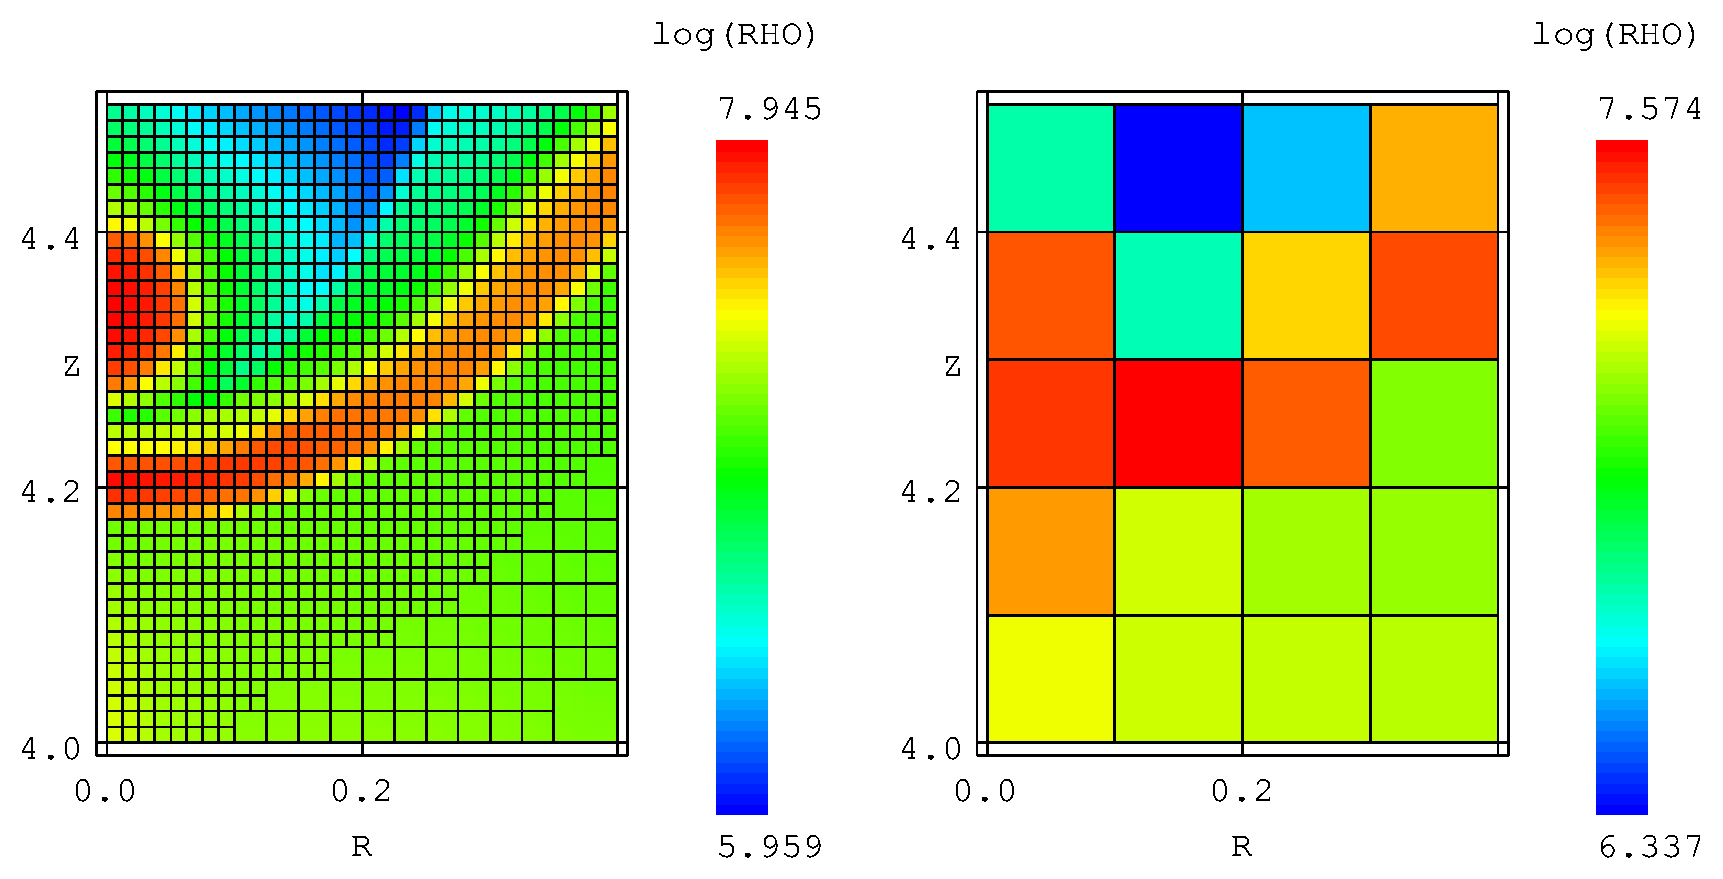
\includegraphics[width=5in]{assets/mergecellc.pdf}
  \caption[Adaptive mesh refinement comparison]{An example of adaptive mesh refinement in the \texttt{MG} hydrodynamical code around the OB star in a colliding wind binary problem using cylindrically symmetric co-ordinates. With AMR the WCR is properly resolved, while without the system cannot adequately resolve the WCR.}
  \label{fig:mgrefine}
\end{figure}

In order to resolve this resolution issue, using cells more effectively than brute-force increasing the resolution must be performed, as such, algorithms such as Adaptive Mesh Refinement (AMR) were introduced to the field of numerics with almost immediate uptake.
AMR is a flexible method of mesh refinement, first discussed by \textcite{bergerAdaptiveMeshRefinement1984} and expanded upon by \textcite{bergerLocalAdaptiveMesh1989}.
This method starts with a ``coarse'' grid at the lowest defined resolution, and tests each cell against a series of conditions, such as proximity to an object in the simulation, conserved parameter or truncation error; if the cell passes any of these threshold conditions it is flagged for refinement.
At the end of a simulation step, the AMR algorithm will split the cell in half along each axis, increasing the effective resolution of the cell.
Conversely, a region can be flagged for de-refinement, where the cells are merged together again, if a condition was transient and is no longer being passed.
Figure \ref{fig:mgrefine} shows this effect, the application of mesh refinement greatly increasing the resolution of of the WCR, allowing for the space between the star and the WCR to be properly resolved, which is crucial for the physically accurate simulation of the CWB.

The benefit of this refinement on systems with only small regions requiring high resolutions is immediately apparent.
In the case of the previously described system with \SI{1.07e12} cells, na\"ively refining a region around 1.5 times the orbital separation from the barycentre with 7 refinement levels reduced the number of cells in the simulation to \num{1.55e6} cells, a 6 order of magnitude reduction in cell count and memory usage.
Care must be taken, however, not to over-refine the simulation or to rapidly refine and de-refine a region.
The former can be mitigated by defining a maximum refinement level, while the latter can be mitigated by defining a minimum number of timesteps required for a cell to be repeatedly flagged for refinement and de-refinement.
% //TODO Check with Julian 
Another issue with this method is multiple refinements per timestep for a cell, which can render the simulation unstable.

In the case of \athena{} meshblocks are instead refined or de-refined, whilst this improves multi-threaded performance with multiple CPUs as it reduces the amount of communication required between processor nodes, this method does increase memory requirements, and is not optimal in an idealised case.
Though, as these simulations are being performed on an HPC cluster this is optimal for our case.
% Note current issues with adaptive mesh refinement, why static mesh refinement is suitable for this project
Unfortunately, despite the advantages of AMR over SMR, there is a known issue with \footlink{\athena{}}{https://github.com/PrincetonUniversity/athena/issues/365} which prevents the use of AMR with passive scalars enabled, scalar values are not conserved properly around meshblock interfaces, which can rapidly escalate and result in physical inaccuracy and breakdown of the simulation.
As there was ultimately no time to correct this bug, the decision was made to persist with using Static Mesh Refinement (SMR) for the second papers work, despite a version of the code already being written with AMR in mind.

Static Mesh Refinement operates by refining regions defined in the problem config file or code that can be refined to a higher resolution, which will progressively de-refine beyond this region until the coarse level is reached.
Whilst markedly less flexible, this is still particularly useful for simulations where the resolution requirements remain approximately in the same place spatially.
In the case of CWB systems this is a reasonably good approximation, as the region around the orbit of the stars can be refined to a higher resolution, while progressively de-refining further out from the barycentre.
Due to the comparatively low flexibility of AMR in a block-based hydrodynamical code such as \athena{}, this was a preferable alternative to refactoring our model to work in either \mg{} or a different numerical code such as \texttt{Enzo}.


%//TODO these may need to be converted into more readable pseudocode, maybe a flow diagram?

% \begin{lstlisting}[language=C++]
% // Get cell width
% Real dx = pmb->pcoord->dx1v(0);
% // March through cells in block, checking distance from star to cell
% for (int n = 0; n < NWIND; n++) {
%   for (int k = pmb->ks; k <= pmb->ke; k++) {
%     // Get Z co-ordinate separation from star
%     Real zc  = pmb->pcoord->x3v(k) - star[n].pos[2];
%     Real zc2 = SQR(zc);
%     for (int j = pmb->js; j <= pmb->je; j++) {
%       // Get Y co-ordinate separation from star
%       Real yc  = pmb->pcoord->x2v(j) - star[n].pos[1];
%       Real yc2 = SQR(yc);
%       for (int i = pmb->is; i <= pmb->ie; i++) {
%         // Get X co-ordinate separation from star
%         Real xc  = pmb->pcoord->x1v(i) - star[n].pos[0];
%         Real xc2 = SQR(xc);
%         // Get radial distance from current star to cell
%         Real r2 = xc2 + yc2 + zc2;
%         Real r  = sqrt(r2);
%         // Get approximate number of cells distance
%         int ri = int(r/dx);
%         // If number of cells distance is below threshold, refine
%         if (ri < amr.star_separation) {
%           return 1;
%         }
%       }
%     }
%   }
% }
% \end{lstlisting}

% \begin{lstlisting}[language=c++]
% // Check to see if meshblock contains the stagnation point
% for (int k = pmb->ks; k <= pmb->ke; k++) {
%   // Get Z co-ordinate separation from stagnation point
%   Real zc  = pmb->pcoord->x3v(k) - wcr.pos[2];
%   Real zc2 = SQR(zc);
%   for (int j = pmb->js; j <= pmb->je; j++) {
%     // Get Y co-ordinate separation from stagnation point
%     Real yc  = pmb->pcoord->x2v(j) - wcr.pos[1];
%     Real yc2 = SQR(yc);
%     for (int i = pmb->is; i <= pmb->ie; i++) {
%       // Get X co-ordinate separation from stagnation point
%       Real xc  = pmb->pcoord->x1v(i) - wcr.pos[0];
%       Real xc2 = SQR(xc);
%       // Get radial distance to current cell
%       Real r2 = xc2 + yc2 + zc2;
%       Real r  = sqrt(r2);
%       // Get approximate number of cells between cell and stagnation point
%       int ri = int(r/dx);
%       // If number of cells distance is below threshold, refine
%       if (ri < amr.wcr_separation) {
%         return 1;
%       }
%     }
%   }
% }
% \end{lstlisting}

\section{Datatypes \& visualisation}
\label{sec:visualisation}

\athena{} exports data in a number of data formats, from formatted tables, to \texttt{VTK} files \parencite{VTK4} to the Hierarchical Data Format standard (\texttt{HDF5}) \parencite{hdf5}.
For all numerical grids being exported, the \texttt{HDF5} standard was used as it was easily the most flexible.
In particular, \texttt{HDF5} has native support for \texttt{MPI} parallelised I/O, which negates the need for writing out individual files for the data for each processing node, and generally has a much greater throughput.
A separate, comma-delimited ``history'' filetype was used to store summated values of conserved variables and advected scalars, this was used primarily to determine simulation-wide dust production rates and average grain sizes as the simulation evolved.
The \athena{} input file syntax allows the user to define multiple outputs to be written at a certain elapsed simulation times, as well as periodically writing ``checkpoint'' files for the simulation to resume from.  
For most simulations, this was performed every fraction of an orbit, with checkpoint files and 3D datasets being written every 1/\nth{100} of an orbit, and 2D datasets and ``history'' file updates being written every 1/\nth{1000} of an orbit.

%//TODO section might not be necessary
Data was plotted using a series of custom programmes designed to parse data as quickly as possible, 
the \texttt{Python 3.8} \parencite{10.5555/1593511} plotting library provided in the \athena{} repository was modified to incorporate Delaunay triangulation, instead of interpolating static meshes to the finest level in order to operate correctly with \texttt{Matplotlib} \parencite{Hunter:2007}, data-points are triangulated with each other.
This is a markedly more memory and processing efficient method, as data is not duplicated or smoothed at the interpolation step, and was found to be approximately 2000\% faster.
Whilst this can result in artefacts at low resolutions, the resolution of the simulation was sufficient such that these artefacts were not observed.
The GNU Parallel library was used to batch-process 2D exports \parencite{tange_2021_5523272}, as \texttt{Python} is for the most part single threaded and interpreted it was found to be more effective use Parallel to run multiple python instances at once, each processing a single data file using the command:

\begin{lstlisting}[language=bash]
seq 0 <max> | parallel -j44  "athena_plot.py plot-config.yaml -n {}"
\end{lstlisting}

\noindent
where \texttt{<max>} is the number of simulation files.
The \texttt{Numba} library \parencite{lam2015numba} was also used to improve performance by  JIT\footnote{Just In Time.} compiling, parallelising and vectorising certain steps that were not performant in either \texttt{Python} or \texttt{Numpy} \parencite{harris2020array}.
In this case, \texttt{Numba} was used to restructure numerical array data into a linear series of arrays, performing derived parameter such as dust density and temperature calculations, and matrix co-ordinate transforms.
While this is less straightforward to implement, as many of \texttt{Pythons} data-types cannot be used, this offered a 2 order of magnitude processing speed increase in the case of an 8-core workstation.

For 3D visualisation the \texttt{VisIt} application is used \parencite{HPV:VisIt}.
However for print 2D slices generated using \texttt{Matplotlib} were used. 
The \texttt{Gnuplot} utility \parencite{gnuplot} was used for generating line and scatter plots throughout this thesis, in particular history outputs from \athena{}.
Occasionally, rendering video of the batch processes 2D exports was performed in order to better understand how the systems propagated over time, in order to do this \texttt{ffmpeg} library \parencite{tomar2006converting} was used to render the videos.
For this, the following command was used:

\begin{lstlisting}[language=bash]
cat /*.png | ffmpeg -f image2pipe -framerate 30 -i - -c:v libx264 -vf format=yuv420p output.mp4
\end{lstlisting}

\section{Simulating CWB systems}

% Recap why CWB simulations are so complex 


% How is this performed, processes involved in mapping wind on stars, orbits, how these are performed in the context of \athena{} or numsim in general

\subsection{Assumptions}
\label{sec:simassumptions}

% Short subsection covering assumptions used in this project

% Wind mapping, lack of radiative line driving
Another assumption is that the outflow from each star is rapidly accelerated to the stars wind terminal velocity, $v^\infty$.
This negates the need for simulating radiative line driving effects on the stellar wind, or calculating the CAK parameters for each wind, however this can result in over-estimation of the wind collision velocity if the wind momentum is sufficiently imbalanced, and the apex of the WCR is close to the secondary star.
If the wind velocity is sufficiently reduced this can effect the structure of the wind collision region, as the wind momentum ratio and cooling parameter will be changed.
Additional factors such as sudden radiative braking can also effect the primary star, where in the case of an extremely unbalanced wind, the primary stellar wind can become rapidly decelerated as it approaches the secondary star and its radiative flux is more influential than the driving force of the parent star \parencite{gayley_sudden_1997}.
This should be considered when analysing the results of each simulation, and understanding how the secondary wind velocity can effect the cooling and dust production rate of the WCR.

% Radiation processes

% Short coverage on dust model, this is explained further in a alter section

\subsection{Wind propagation \& refinement}

% Orbits

% Why not gravitational interaction?
As there are only two gravitationally interacting bodies in the system, it was deemed unnecessary to implement a more complex n-body gravitational system to model the dynamics of the stars.
Additionally, calculating the radial velocity at the start of the simulation would be required, all of which is not needed in the case of a Keplerian orbit simulation.
As the orbital path of the system is already known, this also allowed the use of a ``phase offset'' to change the starting point of each simulation, such as in the case of the WR140 simulation, which begins at $\phi = 0.95$.

% Wind propagation
With the assumption that winds are rapidly accelerated to $v^\infty$, propagating stellar winds through a simulation has been drastically simplified.
% Wind remapping
In the simulation, the conserved variables inside a small spherical region 6 fine cells in radius are modified in order to inherent the parameters of a stellar outflow, with a mass loss rate of $\dot{\text{M}}$ and a wind velocity of $v_\infty$ radially outwards from the star.
The conserved variables, correspond to:

\begin{subequations}
  \begin{align}
    \rho_R &= \frac{\dot{\text{M}}}{4 \pi r^2 v_\infty}, \\
    P_R    &= \rho_R v_\infty^*, \\
    E_R    &= \frac{P_R}{\gamma - 1} + \frac{1}{2} \rho_R v_\infty^2,
  \end{align}
\end{subequations}

\noindent
where $r$ is the radial distance from the star, $P_R$ is the cell pressure, and $\gamma$ is the ratio of specific heats, typically $5/3$.
Whilst this method is very fast and effective, it requires the remap region to remain completely undisturbed, if the WCR impinges upon the remap region this will result in significant physical inaccuracy.
In order to mitigate this, it was found that there should be $75-120$ fine cells separating the stars, for a system with $\eta\sim 0.01$.
For systems with a WCR closer to the secondary star the number of cells should be significantly increased.
 
% How refinement is performed 
Throughout this thesis SMR is used to increase the effective resolution of simulations, a box around the CWB orbit is refined to the highest level defined in the simulations input file, \athena{} de-refines the cells gradually around this box until the simulation is at its coarsest resolution.

\subsection{Cooling in numerical simulations}

% Brief recamp on radiative cooling processes, compare with physical section, why they are important in the context of our work
As discussed in section \ref{sec:wcrcooling}, there are many cooling processes that need to be considered when simulating a complex system such as a CWB.

Sufficient cooling is in fact, essential to this dust formation process.
Gas temperature in the immediate post-shock region can exceed $10^8\, \si{\kelvin}$, far beyond the temperatures required to adequately form dust, as any nascent grains would quickly be shattered by thermal processes.
There is sufficient evidence to suggest that significant, rapid temperature loss occurs in the post-shock regime, the high metallicity of the WC wind and high number density of atoms and ions makes it the ideal region for rapid cooling due to radiative processes.

% Why even include cooling
Another boundary to dust formation due to an insufficiently radiative post-shock flow is a lack of sufficient downstream density.
In the case of strong, adiabatic shocks, constraints are set on the downstream gas parameters of the system, such that:

\begin{subequations}
  \begin{align}
    u_b    & = \frac{1}{4} u_a , \\
    \rho_b & = 4 \rho_a , \\ 
    P_b    & = \frac{3}{4} \rho_a u_a^2 ,
  \end{align}
\end{subequations}

\noindent
where $a$ is the upstream side and $b$ is the downstream, post-shock side.
As the gas density can only be a factor of 4 larger than the post-shock flow, the post shock density (even if it were at  temperatures suitable for dust formation) is insufficiently dense for sufficient dust production.
However, in a radiative shock behaving isothermally (where the temperature change, $\Delta T$ throughout the entire lifespan of the fluid is equal to zero), the final density, $\rho_f$ can be approximated to:

\begin{equation}
  \rho_f \approx \gamma M_a^2 \rho_a,
\end{equation}

\noindent
where $M_a$ is the pre-shock mach number.
For a shock with an initial sound speed of $M_a = 100$ the final density can exceed the pre-shock density by a factor of $10^4$!

% Complexities, conservation, that kind of thing

Performing radiative cooling within a numerical simulation is computationally difficult, and trade-offs between accuracy and performance must be considered at every step of designing the simulation, as every single cell must undergo cooling.
For this project, the final cooling can be out by a few percent at worst, but is fast enough to run the simulations in a reasonable amount of time without excessive memory requirements.
In order to simplify the radiation calculations, radiation does not re-interact with the simulation, instead it is completely removed from the simulation.
Due to this, scattering, re-adsorption and radiative transfer are not simulated at all.\footnote{If these are considered, your programme is now a ray-tracing programme as well as a hydrodynamical code, which is its own, even more complicated field.}.
Other methods of reducing computational cost and optimising the code are used in this project, and will be described in detail in this section.

\subsection{Plasma cooling}

% This isn't a section on the radiative processeses themselves, but more to do with how plasma cooling is simulated 

% Mention stuff like MEKAL

% Use of a lookup table
Thus, instead of calculating the emissivity of the plasma for the current density, temperature and abundances, a lookup table is pre-calculated and loaded into the simulation at runtime.
These lookup tables are generated by combining a series of lookup tables generated for pure flows of elements, and combined based on the abundance of the element within the stellar wind, hence each star in the simulation has its own unique lookup table.
A typical lookup table in this project utilises logarithmically spaced temperature bins from $10^4\,\si{\kelvin}$ to $10^9\,\si{\kelvin}$, with 100 bins in total, if the calculated temperature is between bins a linear interpolation step is used to improve the accuracy of the the emissivity solution.
In order to calculate the energy loss due to emission from atoms and ions within a cell, the following formulae is used:

\begin{equation}
  \mathcal{L}\rms{g} = \left(\frac{\rho}{m_H}\right)^2 \Lambda\rms{g} (T) ,
\end{equation}

\noindent
where $\Lambda\rms{g}(T)$ is the normalised emissivity at the cell temperature, T.
This solution is orders of magnitude faster than performing an emissivity calculation in every cell, and is essential to performing fast hydrodynamical simulations with plasma radiative cooling.

% Mean molecular mass


% Improvements to accuracy of lookup table, linear search
Other optimisations relied on replacing a na\"ive linear search with an indexing method that relied on the logarithmic spacing of the temperature bins, instead of performing a search the index, $n$, of the emissivity value stored in an array can be calculated using the formulae

\begin{equation}
    n = \left \lfloor \frac{\log(T) - \log(T)_\text{min}}{\delta \log (T)} \right \rfloor ,
\end{equation}

\noindent
where $\log(T)$ is the log of the cell temperature, $\log (T)_\text{min}$ is the minimum log temperature in the lookup table and $\delta \log (T)$ is the log spacing of the temperature bins. 
This speed-up is fairly significant as the average search performance changes from $\mathcal{O}(n)$ to $\mathcal{O}(1)$ time, a marked improvement over even a binary search, which would resolve in an average of $\mathcal{O}(\log n)$ time.
In the case of a 100 bin array this is only a minor speed-up, but with the sheer number of calculations being performed, any optimisation to a function used multiple times per cell can significantly improve performance.
In the case of larger, or multi-parameter lookup tables this method would only improve in performance, and is a good example of general optimisation in a numerics programme.

% Method of integration chosen
In order to integrate the energy loss rate to determine the exact amount of energy lost within a timestep, an integration method needs to be chosen, for this project, a fast, first-order Euler method with multiple sub-steps was chosen. Whilst this method is not particularly accurate or robust, it was found to be fast, and the adaptive sub-step method was found to calculate a reasonably accurate approximation of a cells change in temperature in a very small amount of time. This sub-step method is elaborated on in section \ref{sec:cooling-implementation}.

% Why is the estimated method used? see: dust cooling, multiple winds
Other methods of refining the emissivity value were also considered, such as fitting a local curve to the data or using a spline-based interpolation step instead of a linear step, however these were only marginally more accurate, at a significantly increased calculation time. 
An exact cooling method was also considered, which was found to be significantly more performant, but had a series of limitations that prevented it from being used in the codebase at this time.
% Explanation of method, complex bit
This exact cooling method, described by \textcite{townsendExactIntegrationScheme2009}, introduces a temporal evolution function (TEF), $Y(T)$, into the solution, which describes a measure of the total time required to cool from an arbitrary temperature to $T$.
This function, as well as its inverse, need to be calculated prior to cooling being calculated, but do not have to be calculated for every cell and timestep, while solving the TEF for the cell temperature takes approximately the same amount of time as a single first order Euler method integration, whilst offering an \textit{exact} calculation of the post-step temperature.
% Why would this be good
This scheme is one of the rare example of a numerical method that is both accurate \textit{and} fast, taking approximately the same time as a second order explicit method overall, whilst also being perfectly accurate even in highly radiative hypersonic flows.
% Why did we not use it
Unfortunately this method has a number of limitations that precluded its usage in this project.
First, this method would not have been able to accurately model mixed wind situations, hampering its usage cooling winds with drastically different abundances.
%//TODO check this one with Julian
Second, and most importantly, dust cooling could not have been modelled with this single parameter TEF method, which would have required using a two stage cooling method, as the gas temperature would not be synchronised between stages, this would have resulted in a highly inaccurate cooling solution, obviating the advantages of the exact cooling method.

\subsection{Dust cooling}
\label{sec:dustcoolingmodel}

% Discuss dust cooling in brief, link to section in background, touch on lambda being dependent on 3 rather than 1 value

We have previously discussed the underlying physics of dust cooling in Section \ref{sec:dustcooling-background}.
In particular, we discussed that photon emission from dust is primarily due to grain heating through collisional excitation, which in turn causes the heated grain to emit radiation in a method approximating a black body.
This produces an approximately continuous spectra, dependent primarily on the grain size, grain temperature and number density of particles in the surrounding fluid.

Gas and plasma emissivity for a wind of a specific elemental composition is only dependent on temperature, $\Lambda\rms{g}(T)$, with a corresponding energy loss rate of $\mathcal{L}\rms{g} (n\rms{H},T) = n\rms{H} \Lambda\rms{g}(T)$. 
This is convenient for the sake of calculating gas cooling, as the calculation of the emissivities of thousands of emission lines and multiple radiative mechanisms across a temperature domain from $10^4\, \si{K}$ to $10^9\,\si{K}$ would be exceedingly computationally demanding.
Instead, we can use a lookup table, as described in the previous section.
Unfortunately, while the calculation of emission rate of a dust grain is simpler and does not depend on many discrete calculations, it is dependent on more parameters, which can change per cell.
We find that the energy loss rate due to dust is calculated by the formulae:

\begin{equation}
  \mathcal{L}\rms{d} = n\rms{w} n\rms{d} \Lambda\rms{d}(\rho\rms{w},a,T) ,
\end{equation}

\noindent
where $r\rms{w}$ is the wind number density and $\rho\rms{w}$ is the wind density. 
Therefore, in order to calculate energy loss due to dust emission, we must either build a far more complex lookup table, or determine methods of calculating energy loss quickly.
In this section we will discuss the pros and cons of both methods, and discuss our final methodology used in this project.

% Why so significant?

When debating whether or not to include a feature in a numerical simulation, we must weigh up the computational cost versus necessity of inclusion.
In the immediate post-shock environment we find that the cooling rate due to dust is significantly higher than the cooling due to gas and plasma ($\mathcal{L}\rms{g} < \mathcal{L}\rms{d}$) by approximately a factor of five (Fig. \ref{fig:postshockcoolcomparison-chapter3}).
Dust cooling therefore can play an important role in the initial cooling of the post-shock cooling, resulting in faster cooling to temperatures suitable for grain growth.
As such, dust cooling should ideally by included in these simulations.

\begin{figure}[h]
  \centering
  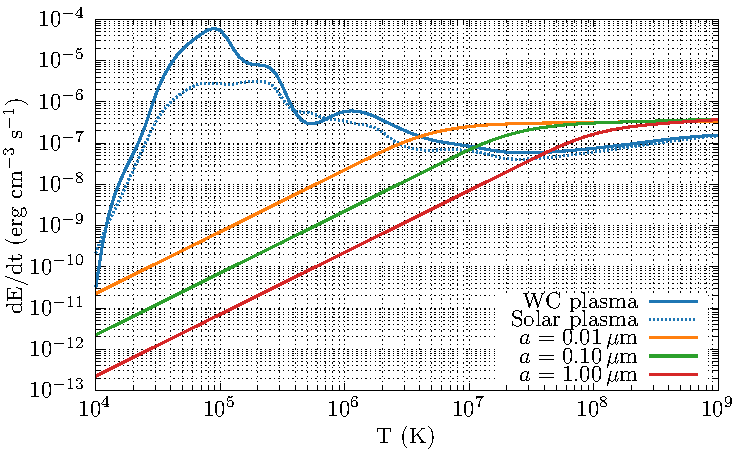
\includegraphics{assets/dust-plasma-cooling-comparison/cooling-comparison-forpaper2.pdf}
  \caption[Comparison of dust and plasma cooling rates in post-shock environment]{Comparison of energy loss due to plasma \& dust cooling with varying grain sizes in a typical post-shock flow, where $\rho_g = 10^{-16} \, \si{\gram\per\centi\metre\cubed}$ and a dust-to-gas mass ratio of $10^{-4}$. Whilst less influential at lower temperatures, dust cooling can aid cooling in the immediate post-shock environment.}
  \label{fig:postshockcoolcomparison-chapter3}
\end{figure}

% Underlying calculation, in depth, 

Throughout this project, we utilise the \textcite{dwek_infrared_1981} prescription for dust radiation emission.
In the case of a dust grain of radius $a$ flowing through a pure elemental gas with an atomic mass $m$ and a number density $n$, 

\begin{equation}
  \begin{split}
    H & = \left(\frac{32}{\pi m}\right)^{1/2} n\pi a^2 (k_B T)^{3/2} h(a,T) \\
    & = \num{1.26e-19} \frac{n}{A^{1/2}} a^2 (\si{\micro\metre}) T^{3/2} h(a,T) \, \si{\erg\per\second}
  \end{split}
\end{equation}

\noindent
where $A$ is the atomic mass of the gas in AMU and $h(a,T)$ is the effective grain heating factor.
This last parameter, also referred to as the grain ``transparency'', is the 

% Effective heating for atoms

% Creati

This critical energy varies depending on the atom and the grain size, and was calculated by \textcite{dwek_infrared_1981} to be 
$23 a^{2/3} (\si{\micro\metre})$ for electrons,
$133a(\si{\micro\metre})$ for hydrogen,
$222a(\si{\micro\metre})$ for helium,
and $665\times a(\si{\micro\metre})$ for metals.
The grain transparency can then be calculated using the formulae:

\begin{equation}
  h(a,T) = 1 - \left(1 + \frac{E^*}{2k\rms{B} T}\right) e^{E^*/k\rms{B}T} .
\end{equation}
% Effective heating for electrons
\noindent
Calculating the grain heating factor for electrons is markedly more difficult, in the uncharged case we find that

\begin{equation}
  \label{eq:heintegral}
  h\rms{e}(a,T) = 1 - \frac{e^{x^*}}{2} \int^\infty_0 \mathcal{K}(x^*,z) dz 
\end{equation}

\noindent
where

\begin{equation}
  \mathcal{K}(x^*,z) = (z + x^*) \left[ (z + x^*)^{3/2} - {x^*}^{3/2} \right]^{2/3} e^{-z} , 
\end{equation}

\noindent
where $x^* = E^* / k\rms{B} T$ and $z$ is an arbitrary value.

% Difficulty of calculating h_e, expand on in integration method subsubsection
Performing an indefinite integral inside of a hydrodynamical code is not ideal, and must be either constrained or simplified in such a way where it can be made performant.
Additionally, electron-grain heating cannot be discounted, as it typically outweighs atom-grain heating more than 2 orders of magnitude (see Section \ref{sec:dustcooling-background}, Fig. \ref{fig:collisionalheatingcomparison}).
% Other difficulty of electrons, free ions
Another factor in determining the contribution due to free electrons was determining the free electron number density, which can vary significantly with temperature in a highly metallic wind.

We trialled two methods involving solving the integral, before settling on using an approximation described in \textcite{dwek_infrared_1981}.

% Difficulties in dust cooling integral, faster method of doing this
\subsubsection{Integration Method}

\begin{figure}[ht]
  \centering
  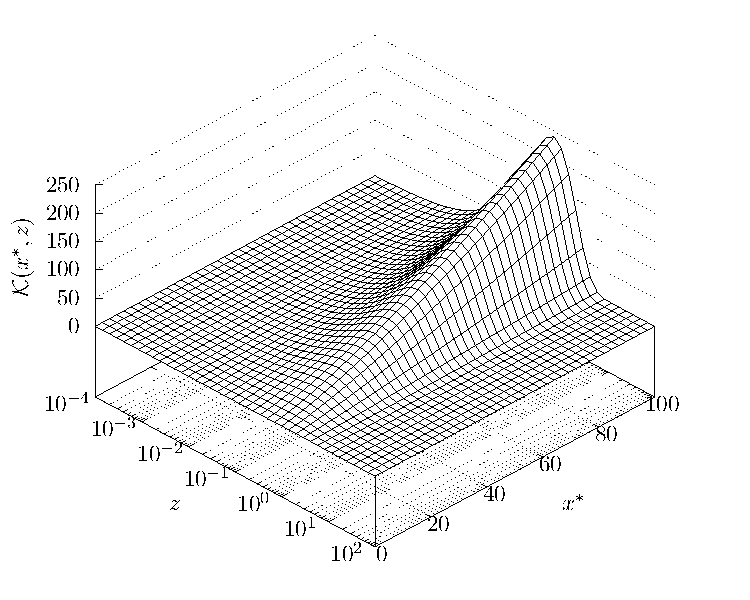
\includegraphics{assets/integral/func_xe_3d.pdf}
  \caption[3D plot of $\mathcal{K}(x^*,z)$]{Surface plot of $\mathcal{K}(x^*,z)$, for a given $x^*$ we can see that $\mathcal{K} \rightarrow 0$ before $z = 100$, suggesting that the integral can be constrained from $z=10^{-3}$ to $z=10^2$.}
  \label{fig:constrainplot3d}
\end{figure}

\begin{figure}[ht]
  \centering
  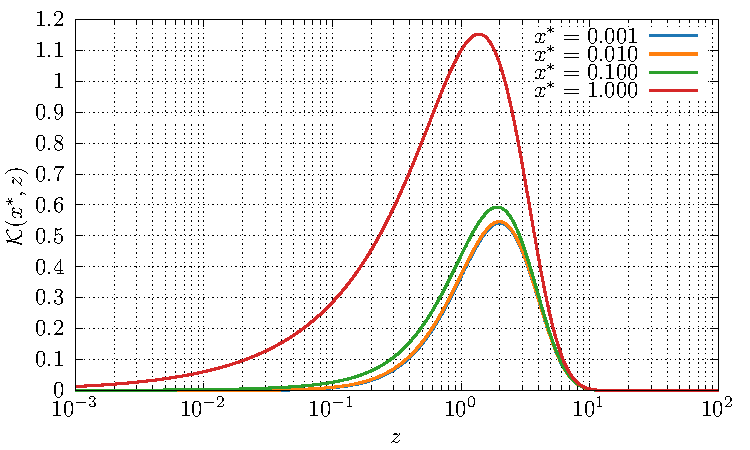
\includegraphics{assets/integral/func_xe_plot.pdf}
  \caption[Plot of $\mathcal{K}(x^*,z)$ for discrete values of $z$]{Plot of $\mathcal{K}(x^*,z)$ with values of $z$ between 0.001 and 1, we see that the plot can moderately well constrained between $z=10^{-3}$ and $z=10^2$.}
  \label{fig:constrainplot2d}
\end{figure}

The first, and most na\"ive method of determining $h_e$ was by calculating an approximation of $h_e$ for each cell at each cooling step.
The integral described in Eq. \ref{eq:heintegral} can be constrained and calculated using a definite integral method such as the trapezium rule.
It was determined that the equation peaks at $z \approx 1$ in all cases, and quickly tapers off to $0$ before $z=100$ (Fig. \ref{fig:constrainplot3d} \& \ref{fig:constrainplot2d}).
The integral was constrained such that

\begin{equation}
  h_e = 1 - \frac{e^{x^*}}{2} \int^{10^2}_{10^{-2}} \mathcal{K}(x^*,z) dz,
\end{equation}

\noindent
and solved through the trapezium method with logarithmically spaced bins.
While this integral can be constrained in such a manner, it was found that a large number of bins was required to solve the equation correctly (Fig. \ref{fig:he-accuracy-bins}).
It was found that 400 bins was the minimum amount required to reliably calculate $h_e$, which would result in the integral taking approximately 90\% of the overall execution time of the cooling step.
Values below 400 bins would result in negative values for $h\rms{e}$, which would render the simulation completely unphysical.
Subtle improvements to performance could be made by forcing $h
rms{e} = 1.0$ for temperatures below $10^6 \, \si{K}$, but this was found to still be comparatively slow.
A more complex integration method would not improve performance at this point, instead, other methods were considered.

\begin{figure}[ht]
  \centering
  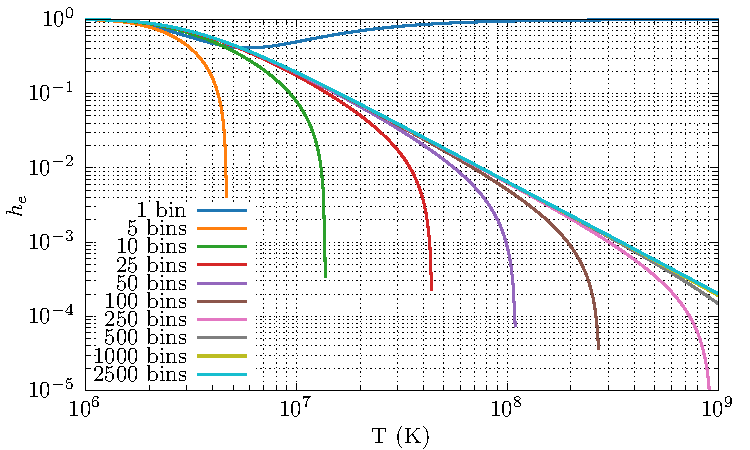
\includegraphics{assets/he_accuracy/he_acc.pdf}
  \caption[$h_e$ integration accuracy comparison]{Comparison of $h_e$ as a function of temperature for dust grains with a radius of 0.005 \si{\micro\metre}, $h_e$ is calculated via the trapezium rule with a varying number of bins, bin counts below 400 bins result in wildly inaccurate or in some case negative values for $h_e$, while beyond 400 bins the result is accurate and converges slowly.}
  \label{fig:he-accuracy-bins}
\end{figure}

\subsubsection{Lookup table}

Another method considered was the use of a multidimensional lookup table, containing values for $\Lambda\rms{d}$ for specific values of $\rho\rms{g}$, $T$ and $a$.
A moderately sized array of $101\times 101 \times 101$ elements was used, with a total of 1030301 possible values of $\Lambda\rms{d}$, spaced logarithmically.
The values for $\Lambda$ were generated from the integral method of solving Eq. \ref{eq:heintegral} using a \num{10000} bin integration with a parameter space described in Table \ref{tab:lookupparams}.

\begin{table}[ht]
  \centering
  \begin{tabular}{llll}
  \hline
  Parameter & Min & Max & Bins \\ \hline
  $\rho\rms{g}$ & \SI{1e-25}{g.cm^{-3}}   & \SI{1e-10}{g.cm^{-3}}  & 101 \\
  $T$           & \SI{1e4}{K}               & \SI{1e9}{K}            & 101 \\ 
  $a$           & \SI{1e-3}{\micro\metre} & \SI{1e2}{\micro\metre} & 101 \\
  \hline
  \end{tabular}
  \caption{Parameter space of $\Lambda\rms{d}$ 3-parameter lookup table.}
  \label{tab:lookupparams}
\end{table}

Similarly to the 1D lookup table used for gas cooling, for each parameter, $P$, we determine the closest value smaller than ($P\rms{l}$) and greater than ($P\rms{u}$) the actual value.
This is then used to calculate an offset, $P\rms{d}$:

\begin{equation}
  P\rms{d}=\frac{P-P\rms{l}}{P\rms{u}-P\rms{l}} , 
\end{equation}

\noindent
these offsets are then used to perform a trilinear interpolation to calculate $\Lambda\rms{d}$ from the lookup table, through the equation:

\begin{equation}
  \begin{split}
    \Lambda\rms{ll} &=\Lambda\rms{lll}\left(1-\rho\rms{d}\right)+\Lambda\rms{ull} \rho\rms{d}, \\
    \Lambda\rms{lu} &=\Lambda\rms{llu}\left(1-\rho\rms{d}\right)+\Lambda\rms{ulu} \rho\rms{d}, \\
    \Lambda\rms{ul} &=\Lambda\rms{lul}\left(1-\rho\rms{d}\right)+\Lambda\rms{uul} \rho\rms{d}, \\
    \Lambda\rms{uu} &=\Lambda\rms{luu}\left(1-\rho\rms{d}\right)+\Lambda\rms{uuu} \rho\rms{d}, \\
    \Lambda\rms{l} &=\Lambda\rms{ll}\left(1-a\rms{d}\right)+\Lambda\rms{ul} a\rms{d}, \\
    \Lambda\rms{u} &=\Lambda\rms{lu}\left(1-a\rms{d}\right)+\Lambda\rms{uu} a\rms{d}, \\
    \Lambda\rms{d} &=\Lambda\rms{l}\left(1-T\rms{d}\right)+\Lambda\rms{u} T.
  \end{split}
\end{equation}

\noindent
This method is markedly faster, and can be improved if multiple cooling sub-steps are performed.
As the same offset, upper and lower values for $\rho\rms{g}$ and $a$ , as they are invariant over a time-step in any given cell.
Further improvements through handwritten unrolled loops and optimisation for SIMD were performed to improve performance by a factor of two.
This final bilinear+linear method improves performance from the integral method by approximately \num{1800}\%, and can scale well within a numerical simulation (Fig. \ref{fig:dust-opt-speedup}).

\begin{figure}[ht]
  \centering
  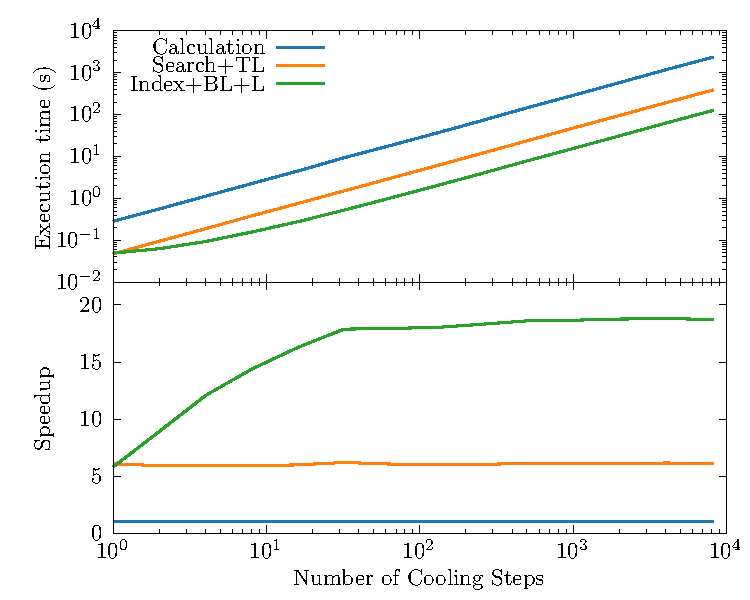
\includegraphics{assets/lambda-dust-speedup/lambda-dust-speedup.pdf}
  \caption[Dust lookup table methods comparison]{Comparison of execution time and speedup for lookup table methods.}
  \label{fig:dust-opt-speedup}
\end{figure}

\subsubsection{\textcite{dwek_infrared_1981} approximation}

\textcite{dwek_infrared_1981} provide a series of equations to estimate $h\rms{e}$ based on the value of $x^*$:

\begin{equation}
  \begin{alignedat}{3}
    h_e(x^*) & = 1 ,                && ~~ x^* > 4.5, \\
    & = 0.37{x^*}^{0.62} , && ~~ x^* > 1.5 , \\
    & = 0.27{x^*}^{1.50} , && ~~ \text{otherwise.}
  \end{alignedat} \label{eq:electrontransparencyestimate}
\end{equation}

\noindent
This method is less accurate, especially between cases, but is multiple orders of magnitude faster.
We find this estimate is at worst divergent from the integral method by $8\%$, and closely matches the results from the integral method (Fig. \ref{fig:lambda-comp-int-vs-est}).
After some optimisation, the resultant estimate was found to be approximately \num{25000}\% faster than the integral method, meaning the electron contribution to dust cooling has a negligible impact on processing time of a single time-step.
Table \ref{tab:electron-speedup} shows the results of benchmarking attempts on all of the methods tested, as we can see, the approximation method is by far the fastest method, with an acceptable worst-case deviation from the integral method result.
Because of this, it was decided that the approximation method would be used.

\begin{figure}[ht]
  \centering
  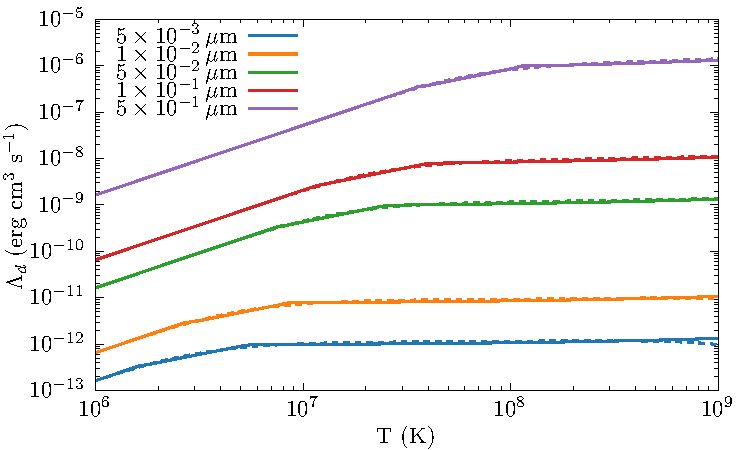
\includegraphics{assets/grain-transparency/lambda-comp.pdf}
  \caption[Electron transparency method accuracy - $\Lambda_d$]{$\Lambda_d$ as a function of temperature for various grain sizes and solar abundances. Solid lines represent calculations from the \textcite{dwek_infrared_1981} estimation, dashed lines represent the integral method. The estimation method is extremely close to the integral value aside from at the highest temperatures.}
  \label{fig:lambda-comp-int-vs-est}
\end{figure}

\begin{table}[ht]
  \centering
  \begin{tabular}{lllll}
    \hline
    Method & t(s) & Iter/s & Speedup & Worst result \\ \hline
    400-bin integration & 36.03 & 35,526 & - & 0\% \\
    Trilinear & 6.016 & 212,751 & 599\% & 0.3\% \\
    Bilinear + linear & 1.999 & 640,447 & 1,803\% & 0.3\% \\
    Approximation & 0.147 & 8,693,171 & 24,510\% & 8\% \\ \hline
  \end{tabular}
  \caption[Dust cooling calculation comparison]{Comparison of methods explored for estimating $\Lambda_d(\rho,a,T)$ in cooling code, $10^4$ initial values were chosen and 128 cooling sub-steps were performed, benchmark code was compiled and run using \texttt{GCC 10.3.0} with the \texttt{-O3} optimisation set on an Intel i7-7700HQ processor with a maximum clock speed of \SI{3.8}{\giga\hertz}.}
  \label{tab:electron-speedup}
\end{table}

\subsubsection{Calculating $n\rms{e}$}

Initially, a solar abundance approximation of the electron number density, $n\rms{e}$, was used, where $n\rms{e} = 1.32 n\rms{H}$, where $n\rms{H}$ is the expected number density in a pure hydrogen flow ($n\rms{H} = \rho\rms{g} / m\rms{H}$).
This can vary as much as a factor of 3 in the case of a WC wind, and vary significantly from $10^4 \, \si{K} \rightarrow 10^7 \, \si{K}$ as the wind becomes increasingly ionised.
A logarithmically spaced lookup table similar to the plasma cooling curve was used, containing the electron-to-ion ratio between $10^4$ and $10^9$ kelvin for both winds (Fig. \ref{fig:electron-curve-no-elements}). 
This method was found to be comparatively fast, as the index method and calculation of the ion number density are computational trivial.

\begin{figure}[h]
  \centering
  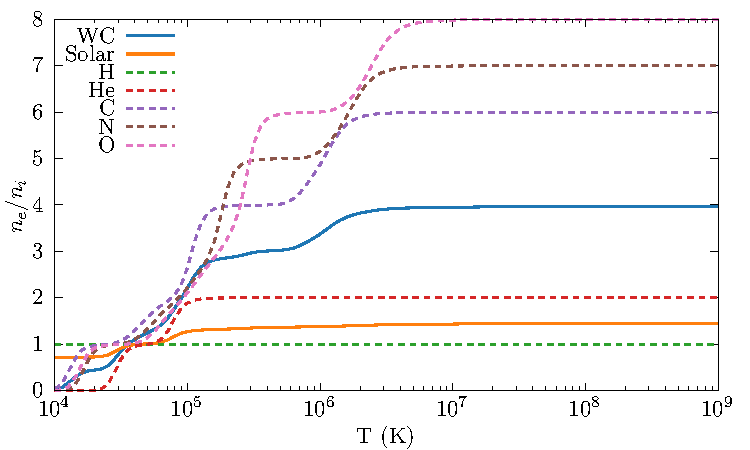
\includegraphics{assets/ionisation-fraction/ionisation-fraction.pdf}
  \caption[OB and WR electron-ion ratios]{A comparison of the electron-ion ratio in both winds as as a function of temperature. Also shown are the electron-to-ion ratios for the individual elements.}
  \label{fig:electron-curve-no-elements}
\end{figure}

\subsection{Model implementation}
\label{sec:cooling-implementation}

In order to simulate energy loss due to radiation in \athena{}, the conserved variable array is adjusted to remove energy from a specific cell, this is analogous to energy being removed from the system due to radiative processes in an optically thin gas.
% Flesh out cooling problem in general
Radiative processes are part of a source function that is performed for every mesh block.
The cooling routine within the source function iterates through all cells within the meshblock, calculating radiative energy loss for each cell.
% Lookup table method recap + how it is applied
Within the loop, the cell parameters are loaded from the conserved variables array, and additional gas and dust parameters are calculated from these conserved variables.
in particular the mean molecular mass of a cell is calculated with the formulae:

\begin{equation}
  \mu = C\mu_{WR} + (1-C) \mu_{OB}, \label{eq:windaveraging}
\end{equation}

\noindent
where $\mu_{WR}$ and $\mu_{OB}$ are the mean molecular masses of the winds and $C$ is the wind ``colour'' scalar, the contribution of each wind to the gas density of the cell.
The temperature is subsequently calculated using the ideal gas law:

\begin{equation}
  T = \frac{P \mu m_H}{\rho k_B}.
\end{equation}

\noindent
At the current temperature, the cooling parameter, $\Lambda\rms{g}(T)$ for each wind is found from the lookup tables, and weighted in a similar manner as equation \ref{eq:windaveraging}. The energy loss due to dust grains is then calculated, with the total energy loss rate per unit volume within the cell defined as:

% \begin{equation}
%   \mathcal{L} = _\text{G} + _\text{D} = \left(\frac{\rho}{m_H}\right)^2 \Lambda_\text{G}(T) + n_\text{D} _\text{grain},
% \end{equation}

\begin{equation}
  \mathcal{L} = \mathcal{L}\rms{g} + \mathcal{L}\rms{d} = \left(\frac{\rho\rms{g}}{m\rms{H}}\right)^2 \Lambda\rms{g} + \left(\frac{\rho\rms{g}}{\mu m\rms{H}}\right) n\rms{d} \Lambda\rms{d}(\rho\rms{g},a,T),
\end{equation}

\noindent
where $\rho\rms{g}$ is the gas density,
$m\rms{H}$ is the mass of a hydrogen atom,
and
$n\rms{d}$ is the dust number density.

% Timestep method, why is this used rather than a single timestep

Performing the exact calculation of $\mathcal{L}$ as described in \textcite{townsendExactIntegrationScheme2009} would only work for gas cooling, and would require significant modification to work with a combination of gas and dust cooling.
Mixed winds are also not supported, and the amount of cooling varies significantly based on the level of metallicity within a system, thus this is significantly less accurate for this use-case.
Adaptive sub-stepping is utilised instead to improve accuracy of a fast Euler integration by increasing the temporal resolution in cases of rapid cooling.
At the end of each sub-step, after $\mathcal{L}$ is calculated, a cooling time is calculated using the formulae:

\begin{equation}
  \tau\rms{cool} = \frac{E_i}{\mathcal{L}} ,
\end{equation}

\noindent
where $E_i$ is the internal energy of the cell.
A fraction of this cooling time is used as a time-step if $\kappa \tau\rms{cool} \leq t\rms{rem}$, where $\kappa$ is a user-defined fraction and $t\rms{rem}$ is the remaining time in the time-step.
This process is repeated until the time-step is completed.
Throughout this project we adopt a value for $\kappa$ of $0.1$.
This method allows for more accurate calculations of cooling in cells with a higher cooling rate, while also being very fast in regions that are not undergoing excessive cooling.
Fig. \ref{fig:cooling-loop-evolution} shows the adaptive sub-stepping routine in operation, at the initial time, the cooling parameter $\Lambda$ is maximised, as such the time-step is significantly lower than when the gas has cooled as is less radiative.
This compares favourably to a single sub-step example, which would cause the simulation to crash due to negative temperatures, and with linearly spaced steps, which either required many more steps or were potentially unstable.

\begin{figure}[ht]
  \centering
  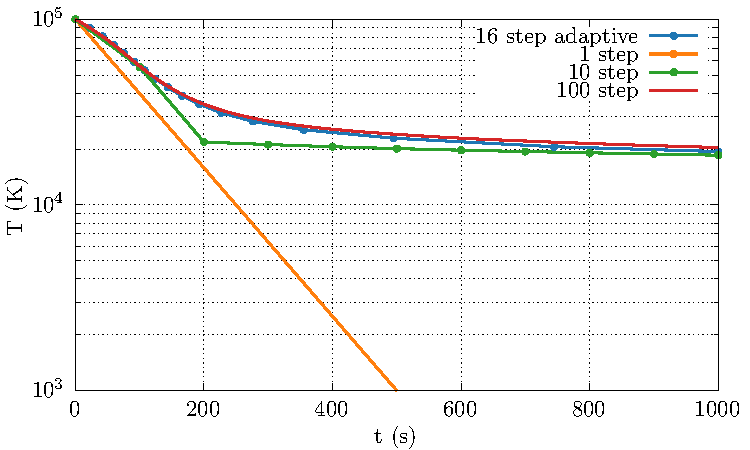
\includegraphics{assets/plasma-cooling-benchmarks/evolution.pdf}
  \caption[Cooling sub-step method evolution comparison]{Comparison of the adaptive timestep method versus linearly spaced sub-steps for a solar abundance flow with a density of $10^{-16}$ \si{\gram\per\centi\metre\cubed} and an initial temperature of $10^5$ \si{\kelvin}. Cooling was artificially limited to prevent negative temperatures, which would have occurred in the case of the 1 sub-step method.}
  \label{fig:cooling-loop-evolution}
\end{figure}

Additional testing with starting temperatures of $10^5 \, \si{K}$, $10^6 \, \si{K}$ and $10^7 \, \si{K}$ and similar parameters to Fig. \ref{fig:cooling-loop-evolution} were used to determine the accuracy of the sub-step method versus the exact integration method proposed in \textcite{townsendExactIntegrationScheme2009}.
$\kappa$ was also varied, in order to determine a suitable value with a reasonable error of no more than $10\%$ at worst. 
Table \ref{tab:cooling-loop-accuracy-comp} shows that $\kappa = 0.1$ produces an error of $6\%$ at worst, while $\kappa = 0.01$ requires an order of magnitude more sub-steps to improve the accuracy to $1\%$.
This is due to the slow convergence time of a first-order integration method such as Euler integration, but this error was deemed acceptable.
At higher temperatures and less intense cooling we find fewer sub-steps are required to calculate $\mathcal{L}$, with much greater accuracy.
A single sub-step took an average of \SI{134}{\nano\second} using the adaptive sub-step method, while the \textcite{townsendExactIntegrationScheme2009} method took \SI{151}{\nano\second}, when conducted on a \SI{3.2}{\giga\hertz} M1 ARM processor with \texttt{O3} optimisation.
The speed benefit of the estimation method is diminished at lower temperatures, but is necessary considering the limitations of the \textcite{townsendExactIntegrationScheme2009} method.
Whilst this is a fairly simplistic method of performing adaptive sub-stepping, it is fast, effective, and not prone to failure.
Improved models in the future could utilise an adaptive RK method, in a similar manner to the numerical integrator in \athena{}, though the implementation attempted had some numerical stability and execution time issues, and would require significant optimisation.

\begin{table}[h]
  \centering
  \begin{tabular}{lllllll}
  \cline{2-7}
   & \multicolumn{2}{l}{$\kappa = 0.1$} & \multicolumn{2}{l}{$\kappa = 0.01$} & \multicolumn{2}{l}{$\kappa = 0.001$} \\ \hline
  $T_i$ & Steps & Error & Steps & Error & Steps & Error \\
  \hline
  $\SI{1e5}{\kelvin}$ & 16 & \num{6.025e-02} & 159 & \num{1.282e-02} & 1585 & \num{7.637e-03} \\
  $\SI{1e6}{\kelvin}$ & 1 & \num{8.233e-04} & 6 & \num{1.012e-04} & 58 & \num{3.359e-05} \\
  $\SI{1e7}{\kelvin}$ & 1 & \num{1.577e-07} & 1 & \num{1.577e-07} & 2 & \num{1.411e-07} \\ \hline
  \end{tabular}
  \caption[Cooling method accuracy comparison]{Accuracy of the adpative sub-step Euler method compared with the \cite{townsendExactIntegrationScheme2009} exact cooling method, with $\kappa = 0.1$ this method is out by $6\%$ at worst in the low-temperature example, while very accurate at higher temperatures with only a single step needed.}
  \label{tab:cooling-loop-accuracy-comp}
\end{table}

\section{The \bidmas{} Advected Scalar Dust Model}
\label{sec:bidmas}

For this thesis, it was decided from the beginning to implement a dust model within a numerical simulation.
This dust model would operate first with advected scalars, before moving on to a more complex multi-fluid model.
Additionally, this model was designed be extensible, implementing grain destruction and accretion mechanisms that were the most influential first.
The Binary Interaction Dust Model with Accretion and Sputtering (\bidmas{})\footnote{Any good thesis (though this one, again, is of debatable quality) has an incredibly laboured acronym!} model is the result of this work, and while in a relatively simple state due to the previously stated time restrictions, is a good first step towards modelling WCd systems.

\subsection{\bidmas{} features}

% Broad featureset
Currently the \bidmas{} model supports grain advection and destruction, as well as the dust cooling model discussed in Section \ref{sec:dustcoolingmodel}.
The main mechanisms changing the quantity of dust in the system are gas-grain accretion, gas-grain sputtering and collisional radiative cooling.
% Species
Furthermore, amorphous carbon is the only species of dust grain considered in this simulation, as it is observed to consist of an overwhelming, if not total, fraction of dust in WCd systems.
% Dust accretion mechanism
Gas-grain accretion occurs with low-velocity collisions between carbon atoms and dust grains.
Grain-grain collision is not simulated as it was determined to occur with significantly less frequency than gas-grain collisions, whilst also being difficult to implement without a grain size distribution.
% Dust destruction mechanism
Dust destruction via gas-grain sputtering occurs when ions with a high thermal velocity collide with the dust grains.
A small amount of material is ablated from the surface of the grain, shattering is not simulated for similar reasons to grain-grain collisions.
% Deciding
The decision of which mechanisms to simulate for each cell are based on the cell temperature, growth mechanisms occur at lower temperatures while destruction mechanisms occur at higher temperatures.
% Conservation
The \bidmas{} model assumes that all gas accreted from dust comes from the stellar wind, therefore any accreted material is subtracted from the gas density of the cell.
% Some issues with numerical instability 
This did present issues initially when developing the model, as on occasion this would result in runaway dust accretion.
% Dust cooling
Finally, dust cooling utilises the model described in Section \ref{sec:dustcoolingmodel}. 

% Lack of a reliance on ``magic numbers''
Another important consideration for this work was a lack of reliance on ``magic numbers'', and for the code to be as well documented as possible.
The initial conditions of the model were based on sensible values for the initial size of grain nuclei and dust mass fractions, as we will discuss in the next section.
Whilst much of the work in this thesis was accomplished on a slightly earlier build of this model, a more advanced, cleaned up version of the model has been implemented.
This improved model is ready for when the AMR stability issues of \athena{} have been solved by the developers.

\subsection{Implementation}



% Passive scalar 
At its most fundamental level, \bidmas{} uses advected scalars\footnote{At times called passive scalars, particularly in the \athena{} documentation. These terms are considered to be interchangeable.} to model dust.
An advected scalar behaves like a tracer or dye in a physical fluid, and for a particular scalar of species $i$, evolves through the simulation with the equation:

\begin{equation}
  \label{eq:advection}
  \rho \frac{dC_i}{dt} = \frac{\partial}{\partial t} \left( \rho C_i \right) + \nabla \cdot \left( C_i \rho \mathbf{u} \right) = -\nabla \cdot \mathbf{Q}_i ,  
\end{equation}

\noindent
where $\mathbf{Q}_i$ is the diffusive flux density of the species:

\begin{equation}
  \mathbf{Q}_i = - \nu\rms{AS} \rho \nabla C_i
\end{equation}

\noindent
and $\nu\rms{AS}$ is the advected scalar diffusion coefficient \parencite{stoneAthenaAdaptiveMesh2020}.
For this work a value of $\nu\rms{AS} = 0$ was used.
As there is no diffusion Eq. \ref{eq:advection} takes the form of the momentum conservation equation, and as such all scalars are co-moving with the gas \parencite[Ch.~10]{toro_riemann_2013}.
Multiple scalars are used to describe the wind and dust parameters within each cell of a simulation:

\begin{itemize}
  \item \texttt{scal\_0}: The wind ``colour'', $C$, or mass fraction of each wind. 
  \item \texttt{scal\_1}: The dust-to-gas mass ratio, $z = \rho\rms{d}/\rho\rms{g}$.
  \item \texttt{scal\_2}: The average grain radius, $\bar{a}$, in microns.
\end{itemize}

\noindent
This method is markedly simpler to implement and faster  to computer, as the dust can be described on a per-cell basis in a series of simple calculations, this allows dust evolution mechanisms to be implemented easily, as long as they can be defined by these parameters either directly or through a derivative, such as the grain number desnity.

\subsubsection{Dust injection}
\label{sec:injection}

\begin{figure}[ht]
  \centering
  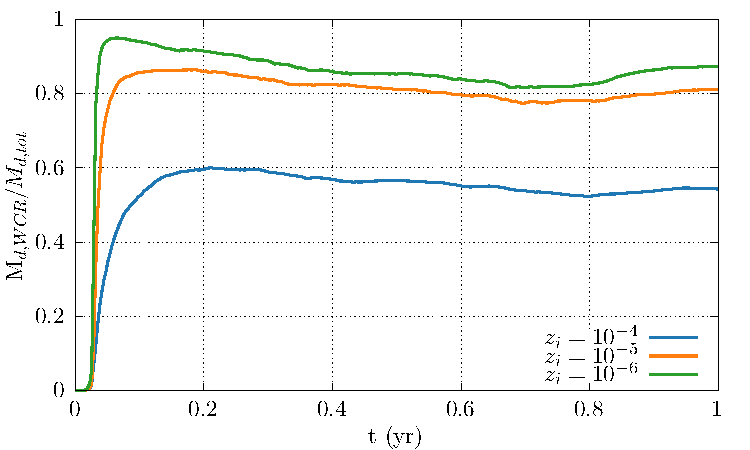
\includegraphics{assets/a_z_tweaking/wcrratio.pdf}
  \caption[WCR dust fraction testing comparison]{A comparison of the WCR dust fraction ($\mass\rms{WCR}/\mass\rms{tot}$) over the course of a simulation with WR98a properties. As $z_i$ deceases the amount of dust produced outside of the WCR decreases significantly. This is consistent across all grain sizes, and does not result in a significantly increased amount of dust.}
  \label{fig:aztwek_wcrrat}
\end{figure}

\begin{figure}[ht]
  \centering
  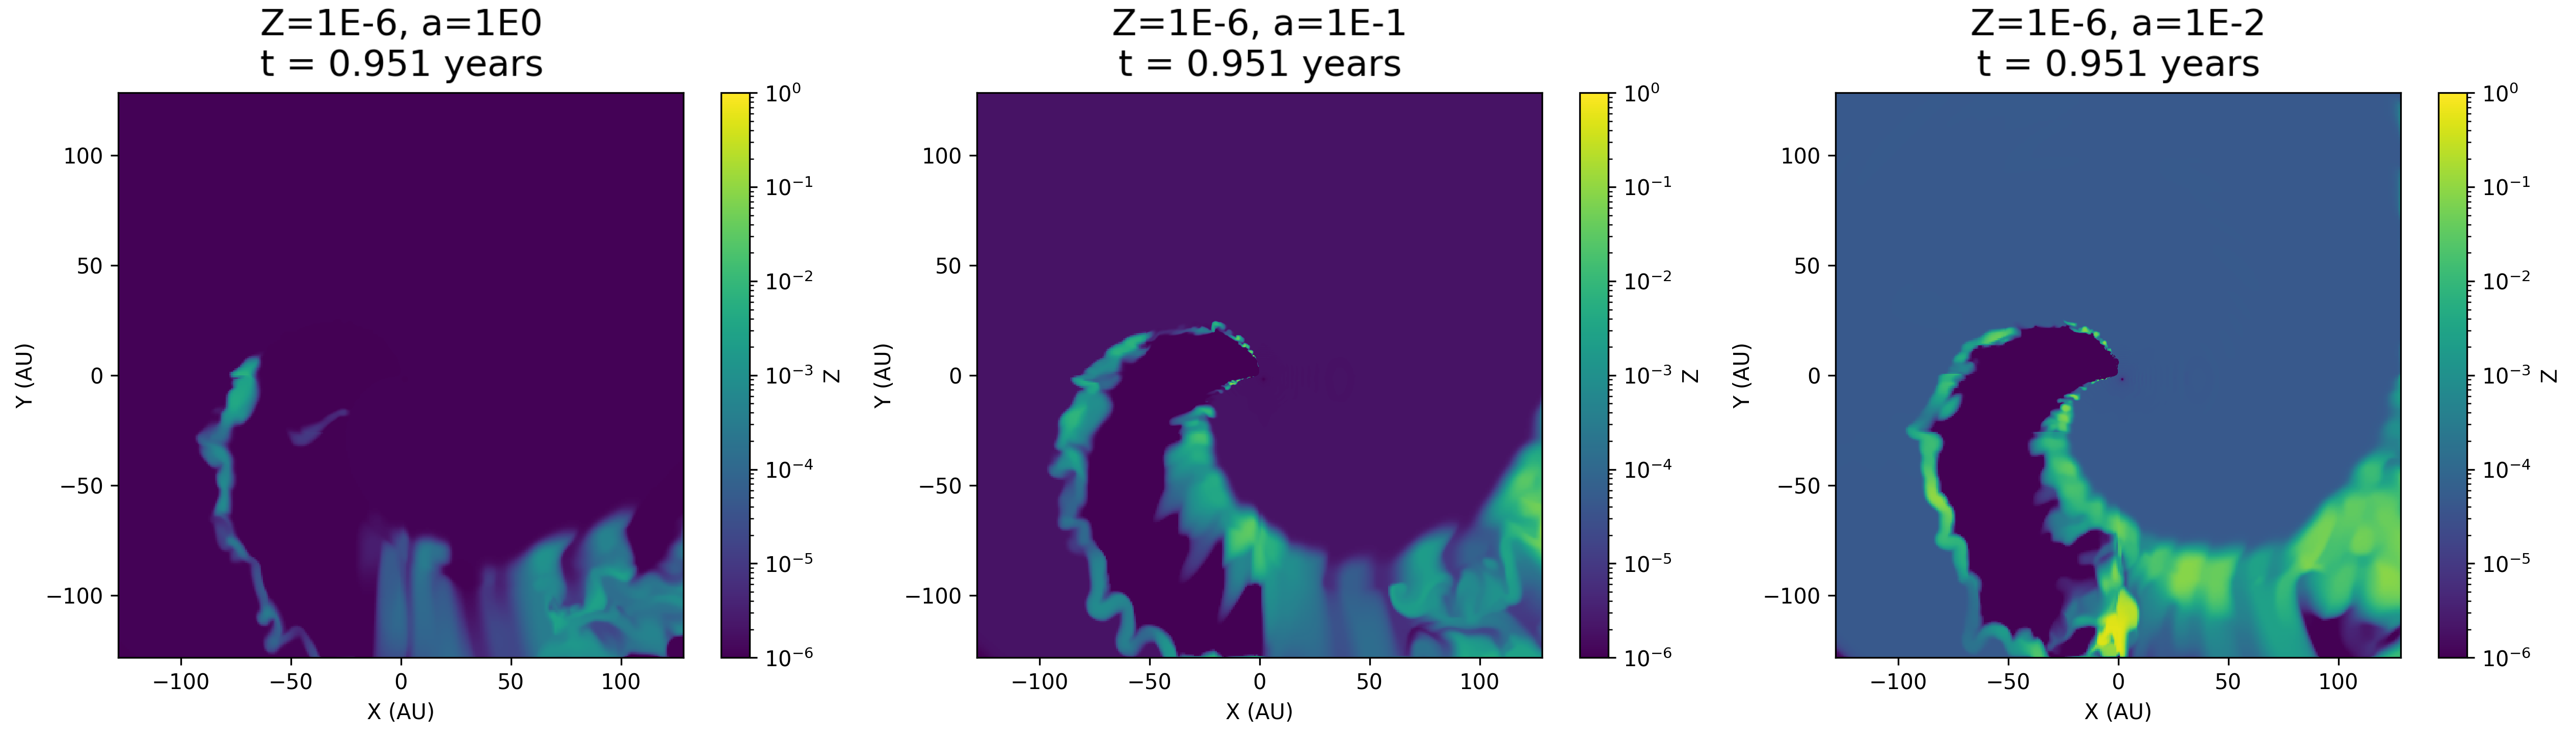
\includegraphics[width=\linewidth]{assets/a_z_tweaking/zconcat.png}
  \caption[$z_i$ testing]{A comparison of WCR dust distribution when $a_i$ is varied in a system with WR98a parameters. Dust yield increases significantly if a smaller, realistic initial grain size is chosen.}
  \label{fig:azweak_img}
\end{figure}

\begin{figure}[p]
  \centering
  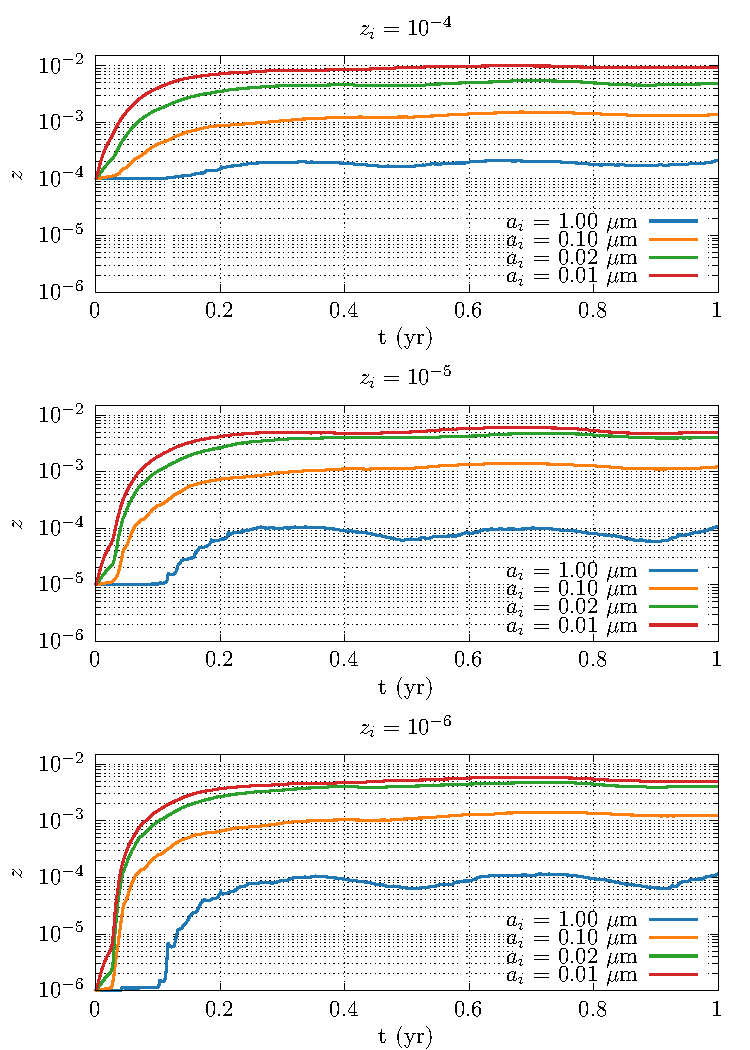
\includegraphics{assets/a_z_tweaking/z.pdf}
  \caption[$z_i$ and $a_i$ parameter tweaking]{A comparison of $z$ over the course of a simulation with WR98a properties, $z_i$ and $a_i$ are varied for each simulation. We find that dust yield increases significantly if a smaller, realistic initial grain size is chosen. Varying $z_i$ does not result in a corresponding change in dust yield.}
  \label{fig:azweak_z}
\end{figure}

Dust is injected into the system in small quantities from the wind remap zone of the WC star.
If we were to describe this mechanism in physical terms, this would be as if refractory carbon grain cores condensed from the WC wind.
Whilst the exact mechanism for initial grain nucleation is not known, this is an ideal first step as it assures that dust grains are present in the post-shock WCR wind.
Another important consideration of this model was for it to be fairly general purpose, and not require significant degrees of initial parameter ``hunting'' in order to simulate a new system.
As such it was decided that the model would operate on as few initial parameters as possible.
% INitial comparisons
Determining the injected scalar values at this remap zone was an important first step, as it was not known how these initial parameters would impact the final dust yield, $\mass\rms{d,f}$, or the dust formation rate, $\mdot\rms{d}$. 
In order to determine the ideal initial parameters, and to determine the sensitivity of the model to it's initial conditions, a series of simulations were conducted using the orbital and wind parameters of WR98a.
The initial grain radius, $a_i$ was varied from \SI{0.01}{\micro\metre} to \SI{1}{\micro\metre}, while the initial dust-to-gas mass ratio, $z_i$ was varied from $10^{-6}$ to $10^{-4}$.
These simulations were run over the course of a week on the ARC4 HPC cluster over 128 cores.
The total elapsed time within the simulation was one year, with the simulation advecting fully to the simulation extent of $100\times 100 \times 10 \, \si{\au}$ in around \SI{0.1}{\year}.
Whilst the results of \textcite{lauRevealingEfficientDust2021} had not been published at this time, a final dust-to-gas mass fraction of $\sim 1\%$ was assumed to be an ideal starting point for a model of WR98a.


As can be seen in Fig. \ref{fig:azweak_img}, we find that decreasing $a_i$ creates a much defined WCR, at the cost of increasing dust outside of the WCR.
Dust formation occurs where expected, on the WC edge of the WCR, with the bulk of dust formation occurring within a short distance from the apex of the WCR shock.
Therefore, we must aim for a small grain radius, and not start with large grains.
Additionally, \textcite{zubkoPhysicalModelDust1998a} notes that the initial dust grain nuclei are expected to be extremely small, on the order of \SI{5}{\angstrom}, and rapidly grow to \SI{100}{\angstrom} through interactions of small, charged grains with impinging carbon ions.
This is expanded on in Fig. \ref{fig:aztwek_wcrrat}, where we find that changing $z_i$ significantly affects the amount of dust produced in the WCR compared to the total dust yield.
As we do not observe significant quantities of dust being produced outside of the WCR, we prioritised a small value of $z_i$, so long that it does not influence dust yields.
Finally, Fig. \ref{fig:azweak_z} shows that changing $z_i$ does not affect the total dust yield significantly, and is far more sensitive to changes in $a_i$.
We can therefore discern from these previous two results that $z_i$ should be kept to a fairly small value.

The other parameter, $z_i$, was found to not effect
Overall, it was found that we could reduce the effective initial parameter space of dust in the wind to a single value, $a_i$, which was found to operate best when kept at realistic values.
After this preliminary parameter space exploration, an $a_i$ of \SI{50}{\angstrom} and a $z_i$ value of $10^{-8}$ were settled on.
Whilst these initial parameters were based on an extrapolation of our test data, these initial values were found to be more than adequate.
Other dust injection mechanisms were considered for this project, such as injecting dust into the apex of the WCR.
However, these were found to give inconsistent results when initially tested in the \mg{} hydrodynamical code.

\subsubsection{Assumptions \& limitations}
\label{sec:bidmasassumptions}
\label{sec:bidmaslimitations}

From this we can determine further assumptions for our dust model.
% Number density
We assume that the number density, $n\rms{d}$, is constant throughout the simulation, which is calculated based on the initial grain radius, $a_i$, and initial dust-to-gas mass ratio, $z_i$, injected into the simulation from the primary star.
% Limitations due to this
Because of this, we therefore assume that the net rate of grain shattering and grain agglomeration is zero.
Additionally, the dust number density may not be correctly calculated, which can affect the rate of cooling.
% Multiple grain sizes and coupling
Additionally, we also assume that there is little variation between grain size within the numerical cell.
% Limitations due to this
Whilst other models assume that dust grains are coupled through a drag force, it was found that the dust was effectively coupled to the wind as if it was co-moving (Section \ref{sec:hendrixmodel}).
This may however prevent significant dust mixing in the immediate post-shock region, due to the increased inertia of the dust grains compared to the gas.
% Grain-grain collision
As a single grain size is assumed, dynamics between grains of different sizes, such as grain agglomeration cannot be accurately simulated.
% Fixes
These issues could be addressed with a multi-scalar or multi-fluid model, which is a potential future feature of this project.

All grains in the simulation are assumed to be circular, with a volume, $V\rms{gr}$, of $4/3 \pi a^3$ and a mass, $m\rms{gr} = V\rms{gr} \rho\rms{gr}$, where $\rho\rms{gr}$ is the grain bulk density.
As we assume all dust grains in the simulation are composed of amorphous carbon, we assume a grain density of \SI{3}{g.cm^{-3}}, which is on the upper end of densities expected for amorphous carbon
\parencite{bhattaraiEvolutionAmorphousCarbon2018}.

\subsubsection{Dust cooling}

Dust cooling is handled within the cooling loop, and functions by removing energy from a cell of the simulation.
The gas is assumed to be optically thin to infrared, and is therefore removed from the simulation without re-adsorption.
The emissivity of the grains at the current temperature and radius, $\Lambda(a,T)$, is calculated for each cell, and the rate of energy loss due to dust emission is calculated such that:

\begin{equation}
  \frac{dE}{dt} = n\rms{T} n\rms{d} \Lambda\rms{d}(T,a),
\end{equation}

\noindent
Where $n\rms{T}$ is the total gas number density and $n\rms{d}$ is the dust number density.
Dust cooling, as well as the optimisations needed to run quickly in a numerical simulation, is discussed in significantly more detail in Section \ref{sec:dustcoolingmodel}.

\subsubsection{Dust evolution}

Once the energy loss due to dust emission has been calculated, the growth rate and destruction rate for dust grains in each cell is calculated.
The code loops through every cell in the simulation, first calculating the average mass of the wind in the cell, $\mu$:

\begin{equation}
  \mu = C \left(2 X\rms{WR} + \frac{3}{4} Y\rms{WR} + \frac{1}{2} Z\rms{WR} \right)^{-1} + (C-1) \left(2 X\rms{OB} + \frac{3}{4} Y\rms{OB} + \frac{1}{2} Z\rms{OB} \right)^{-1} ,
\end{equation}

\noindent
where $C$ is the wind ``colour'', and $X,Y,Z$ are the individual wind hydrogen, helium and metal mass fractions, respectively
\parencite{mihalasStellarAtmospheres1978}.
The cell temperature is then calculated using the ideal gas law:

\begin{equation}
  T = \frac{\mu P\rms{g}}{\rho\rms{g} k\rms{B}},
\end{equation}

\noindent
where $P\rms{g}$ is the gas pressure and $\rho\rms{g}$ is the gas density.
Based on the gas temperature, we determine which dust processes occur.
For temperatures above $10^6 \, \si{K}$, dust destruction occurs, while at temperatures below \SI{1.4e4}{K} dust growth occurs instead.
As the dust grains are assumed to be spherical, we can model dust growth and destruction in a unified manner, corresponding to a change in grain radius.
In the case of dust destruction, ions sputter off atoms from the surface of the dust grain, wearing the grain evenly over time, while in the case of accretion, low velocity collisions cause atoms to stick, growing the grain evenly.

For both processes we find a change in the grain radius of $da/dt$, which can be extrapolated to find the rate of change in dust density with the formulae:

\begin{subequations}
  \begin{align}
    \frac{dV\rms{gr}}{dt} & = 4 \pi a^2 \frac{da}{dt} ,\\
    \frac{dm\rms{gr}}{dt} & = \rho\rms{gr} \frac{dV\rms{gr}}{dt} ,\\
    \frac{d\rho\rms{d}}{dt}   & = n\rms{d} \frac{dm\rms{gr}}{dt} ,
  \end{align}
\end{subequations}

\noindent
where $dV\rms{gr}/dt$ is the rate of change in the dust grain volume and $dm\rms{gr}/dt$ is the associated change in dust grain mass.
To simulate dust growth due to grain-gas accretion we use a method from \textcite[Ch.~9]{spitzerPhysicalProcessesInterstellar2008}.
Carbon atoms accrete onto a dust grain at a constant rate, resulting in a change in radius such that:

\begin{equation}
  \label{eq:dustgrowthradiuschange}
  \frac{da}{dt} = \frac{\xi \rho\rms{C} w\rms{C}}{4\rho\rms{gr}} ,
\end{equation}

\noindent
where $\xi$ is the grain sticking factor, $\rho\rms{C}$ is the density of carbon in the wind ($\rho\rms{C} = \rho\rms{g} X(C)$, where $X(C)$ is the carbon mass fraction), and $w\rms{C}$ is the RMS velocity of ($w\rms{C} = \sqrt{3k\rms{B}T / 12 m\rms{H}}$).
Throughout this thesis we use a grain sticking factor of 0.1, though in the case of ionised gas, this value can be as high as 1.
From Eq. \ref{eq:dustgrowthradiuschange} we can derive a corresponding rate of change in the dust density:

\begin{equation}
  \frac{d \rho\rms{d,acc}}{dt} = \pi \xi \rho\rms{C} w\rms{C} n\rms{d} a^2.
\end{equation}

\noindent
Dust destruction is carried out through the \textcite{draineDestructionMechanismsInterstellar1979} prescription.
We estimate an amorphous carbon grain \SI{1}{\micro\metre} to have a lifespan, $\tau\rms{d}$, of \SI{3e6}{\year}.
As described in \textcite{draineDestructionMechanismsInterstellar1979}, with additional work by \textcite{tielens_physics_1994} and \textcite{dwekCoolingSputteringInfrared1996}, this grain lifespan is dependent on the gas density, $n\rms{g}$, as well as the grain radius, taking the form:

\begin{equation}
  \tau\rms{d} = \frac{a}{da/dt} \approx \num{3e6} \frac{a}{n\rms{g}} \, \si{\year} ,
\end{equation}

\noindent
We can rearrange this equation to find a rate of change in grain radius of $da/dt = a / \tau\rms{d}$.
Finally, we find an associated rate of change in the dust density of:

\begin{equation}
  \frac{d \rho\rms{d,sput}}{dt} = -4 \pi n\rms{d} \frac{\rho\rms{gr} a^3}{\tau\rms{d}} = -4\pi n\rms{d} \frac{\rho\rms{gr} n\rms{g} a^2}{\num{3e6}},
\end{equation}

\noindent
In order to find the total change in the dust density, $\Delta \rho\rms{g}$, and the grain radius, $\Delta a$, we perform a Euler integration over the simulation timestep, $\Delta t$:

\begin{equation}
  \Delta x = \int^{t+\Delta t}_{t} \frac{dx}{dt} dt \approx \frac{dx}{dt} \Delta t ,
\end{equation}

\noindent
where $x$ is the quantity being integrated and $t$ is the simulation time.
Whilst a Euler method integration is less accurate than a sub-stepping method or higher-order integration method, this was found to be adequate, as the growth rate of the dust grain was found to be small over a single time step.
After the total change for $\rho\rms{d}$ and $a$ are calculated, the post-step grain radius, $a\rms{new}$, is calculated:

\begin{equation}
  a\rms{new} = a\rms{old} + \Delta a .
\end{equation}

\noindent
Then the post-step dust and gas densities are calculated, with the new dust being subtracted from the fluid:

\begin{subequations}
  \begin{align}
    \rho\rms{d,new} & = \rho\rms{d,old} + \Delta \rho\rms{d} , \\
    \rho\rms{g,new} & = \rho\rms{g,old} - \Delta \rho\rms{d} . 
  \end{align}
\end{subequations}

\noindent
Finally, the new dust-to-gas mass ratio can be calculated from the new dust and gas densities:

\begin{equation}
  z\rms{new} = \frac{\rho\rms{d,new}}{\rho\rms{g,new}} . 
\end{equation}

\noindent
These new scalar values then overwrite the previous scalar values.
Passive scalars in \athena{} are stored in the following arrays for a scalar species \texttt{N} in a meshblock with indices \texttt{i,j,k}:

\begin{itemize}
  \item \texttt{pmb->pscalars->r(N,i,j,k)}: Primitive variables between \texttt{0.0} and \texttt{1.0}.
  \item \texttt{pmb->pscalars->s(N,i,j,k)}: Conserved variables between \texttt{0.0} and \texttt{rho}, the conserved cell density.
\end{itemize}

\noindent
These values have to be updated simultaneously, and occurs at the end of each iteration of the main processing loop such that:

\begin{lstlisting}[language=c++]
  // Update primitive scalars
  pmb->pscalars->r(1,k,j,i) = z_new;  // Update z primitive
  pmb->pscalars->r(2,k,j,i) = a_new;  // Update a primitive
  // Update conserved scalars 
  pmb->pscalars->s(0,k,j,i) = col   * rho_new;  // Update colour conserved
  pmb->pscalars->s(1,k,j,i) = z_new * rho_new;  // Update z conserved
  pmb->pscalars->s(2,k,j,i) = a_new * rho_new;  // Update a conserved
\end{lstlisting}

\noindent
\athena{} automatically re-scales scalar values lower than \texttt{0.0} or greater than \texttt{1.0} or \texttt{rho} (depending on the variable type) at the end of each time-step\footnote{This method also limits the grain size to a maximum radius of \SI{1}{\micro\metre}, but growth of this level outside of testing - where the grain radius was stored in centimetres - was never observed.}.

\subsection{Contemporary dust Models}

At the time of writing, there has been no research conducted that has accomplished all three of the following criteria:

\begin{enumerate}
  \item Models a CWB system using a numerical simulation.
  \item Implements a dust model inside this numerical simulation.
  \item Simulates multiple features such as dust accretion, sputtering and radiative cooling.
\end{enumerate}

\noindent
There are two dust models in particular, however, that should be discussed, as they fulfil some of these conditions.
These are the \textcite{harriesThreedimensionalDustRadiativetransfer2004} and \textcite{hendrix_pinwheels_2016} dust models.
% Ballistic dust model
Research conducted by \textcite{harriesThreedimensionalDustRadiativetransfer2004} involved the simulation of dust emission through a ballistic particle model, with the CWB simulated as a conical region.
Dust of a uniform size of \SI{0.01}{\micro\metre} was used, with the cone being simulated with a radiative transfer model, in order to constrain the dust production rate of the WR104 system through comparison to observations.

\subsubsection{The Hendrix dust model}
\label{sec:hendrixmodel}

Perhaps the most similar contemporary dust model is the model described in \textcite{hendrix_pinwheels_2016} - as this model is concerned with simulating the dynamics of dust within a CWB.
This is not to say that these models are identical, of course, as the Hendrix model explores how dust spreads throughout the WCR of WR 98a, in order to compare with observational data using radiative transfer code.

% Differences between models 

The main differentiating factors between this model and our model are the driving mechanism and dust evolution.
In the Hendrix model dust is modelled as a separate fluid, with an Epstein drag function between the wind and dust fluids; this method allows for dust kinematics that aren't implicitly co-moving.
This is a more accurate method of modelling dust, however it requires significantly more processing time and is much more difficult to implement, requiring a numerical code that supports multiple fluids.
At the start of this PhD this was considered but eventually rejected due to time constraints.

However, the Hendrix model has limitations that this model does not have, this is because the purpose of the Hendrix model is to analyse the distribution of dust within a CWB system, rather than to model the evolution of the dust itself.
To this end, the Hendrix model does not calculate dust growth or destruction, and only uses a single small grain size, with the dust-to-gas mass ratio calculated based on observations of the target system, WR98a.

\subsection{Future dust models}

% Future work, adopt multi-fluid model?

Due to time constraints and limitations in the code in use, only a limited set of mechanisms for dust evolution were included in this projects simulations.
While the \bidmas{} model represents an interesting start for the modelling of dust grains in colliding wind binaries, future models could implement more complex models which incorporate additional destruction and growth mechanisms, as well as a multiple dust grain sizes.

A multiple grain size scalar model could be used to more accurately measure the growth of dust grains, rather than a single average grain size.
This would be more difficult to implement than a single model but would be able to estimate grain-grain collision, and better estimate dust growth and destruction rates.
\athena{} and MG both have issues with a large number of scalars, as such both numerical codes may require significant modification to cope with this.
A multi-fluid model with dust being physically simulated rather than assumed to be perfectly co-moving would be an ideal next step.
Multiple grain size distributions could also be modelled in a similar way to the proposed multi-scalar model, however the kinematics of the dust grains could also be simulated separately.
% Mixing factors
The increased inertia of more massive dust grains could result in the kinematics of the dust flow diverging from the co-moving assumption.
To that end, a successor dust model would adopt a multi-fluid and drag function method, which was considered but not included for the sake of time.
This multi-fluid model would also allow for more physically accurate simulation of grain-gas and grain-grain interactions, as the collision velocities would be exactly calculated rather than estimated through bulk motion properties.
High speed collision of gas on dust grains in the immediate post-shock environment could also shatter grains, though modelling this as well as spalling of particles in the wind through the dust grains would be complex to simulate. 

Furthermore, additional mechanisms for dust destruction, such as through photodissociation and sublimation could also be implemented, the implementation of these could be used to determine the effectiveness of the WCR in protecting nascent, still forming dust grains.

% Better dust nucleation model

The initial grain nucleation model could also be improved, injection of extremely small grains into the simulation through the stellar remap zones was chosen as the underlying chemical process for formulation of these dust grains is poorly understood at the time of writing.
% Current model not too bad, strong dependence on a but z does not change much, being dependent on a single parameter not too bad
The small grain nucleation model was also found to be only dependent on the initial grain radius, $a_i$, whilst changing the amount of grain nuclei in the WR wind does not change the amount of dust produced.
As such the simulations are currently bound by a single input parameter, which can be constrained based on what is currently understood about dust grain accretion.
% Difficulty in picking initial parameters for more complex model
A more complex model may require additional parameters, and as such could be highly dependent on these initial parameters, as such, another round of initial parameter hunting would be required.

% Comparison with observational results

\begin{figure}[ht]
  \centering
  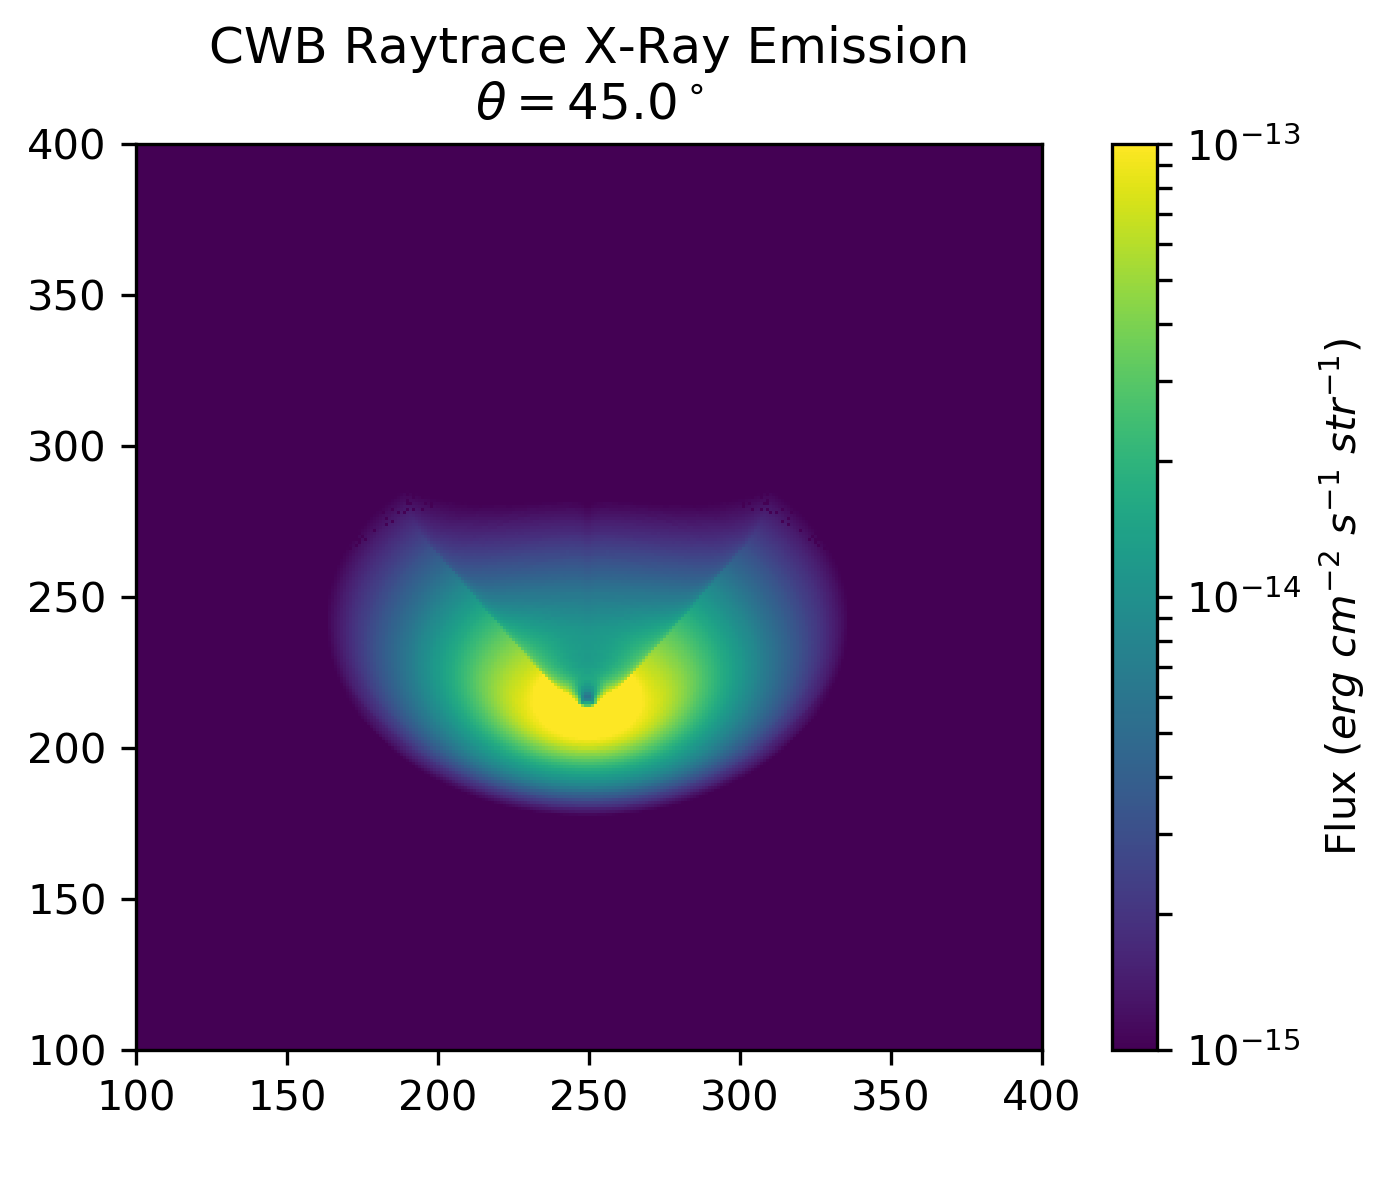
\includegraphics[width=4in]{assets/ray/cwb-raytrace-045.0.png}
  \caption{X-ray radiative transfer image from \SI{0.1}{\kilo\electronvolt} to \SI{10.0}{\kilo\electronvolt} of a test CWB system with a momentum ratio of $\eta = 0.01$ inclined at $\phi = 45^\circ$ from the obesrver at a distance of \SI{1}{\kilo\parsec}. Radiative transfer was performed on an in-house code, which was to be modified to support dust emission.}
  \label{fig:inhousert}
\end{figure}

Another avenue of future research would be performing a radiative transfer simulation upon a fully advected system, in order to compare with observational results.
Whilst some initial tests were performed with in-house x-ray emission code that was to be modified to support dust emission (Fig. \ref{fig:inhousert}).
Using other radiative transfer codes such as \texttt{HYPERION} were also considered \parencite{robitailleHYPERIONOpensourceParallelized2011}, but this was abandoned due to time constraints from changing hydrodynamical codes from \mg{} to \athena{}.
Radiative transfer modelling was performed by \textcite{hendrix_pinwheels_2016}, with the resultant images emulating the sensitivity and angular resolution characteristics of UKIRT, Keck and ALMA (figure \ref{fig:hendrix-synthetic}).

\begin{figure}[ht]
  \centering
  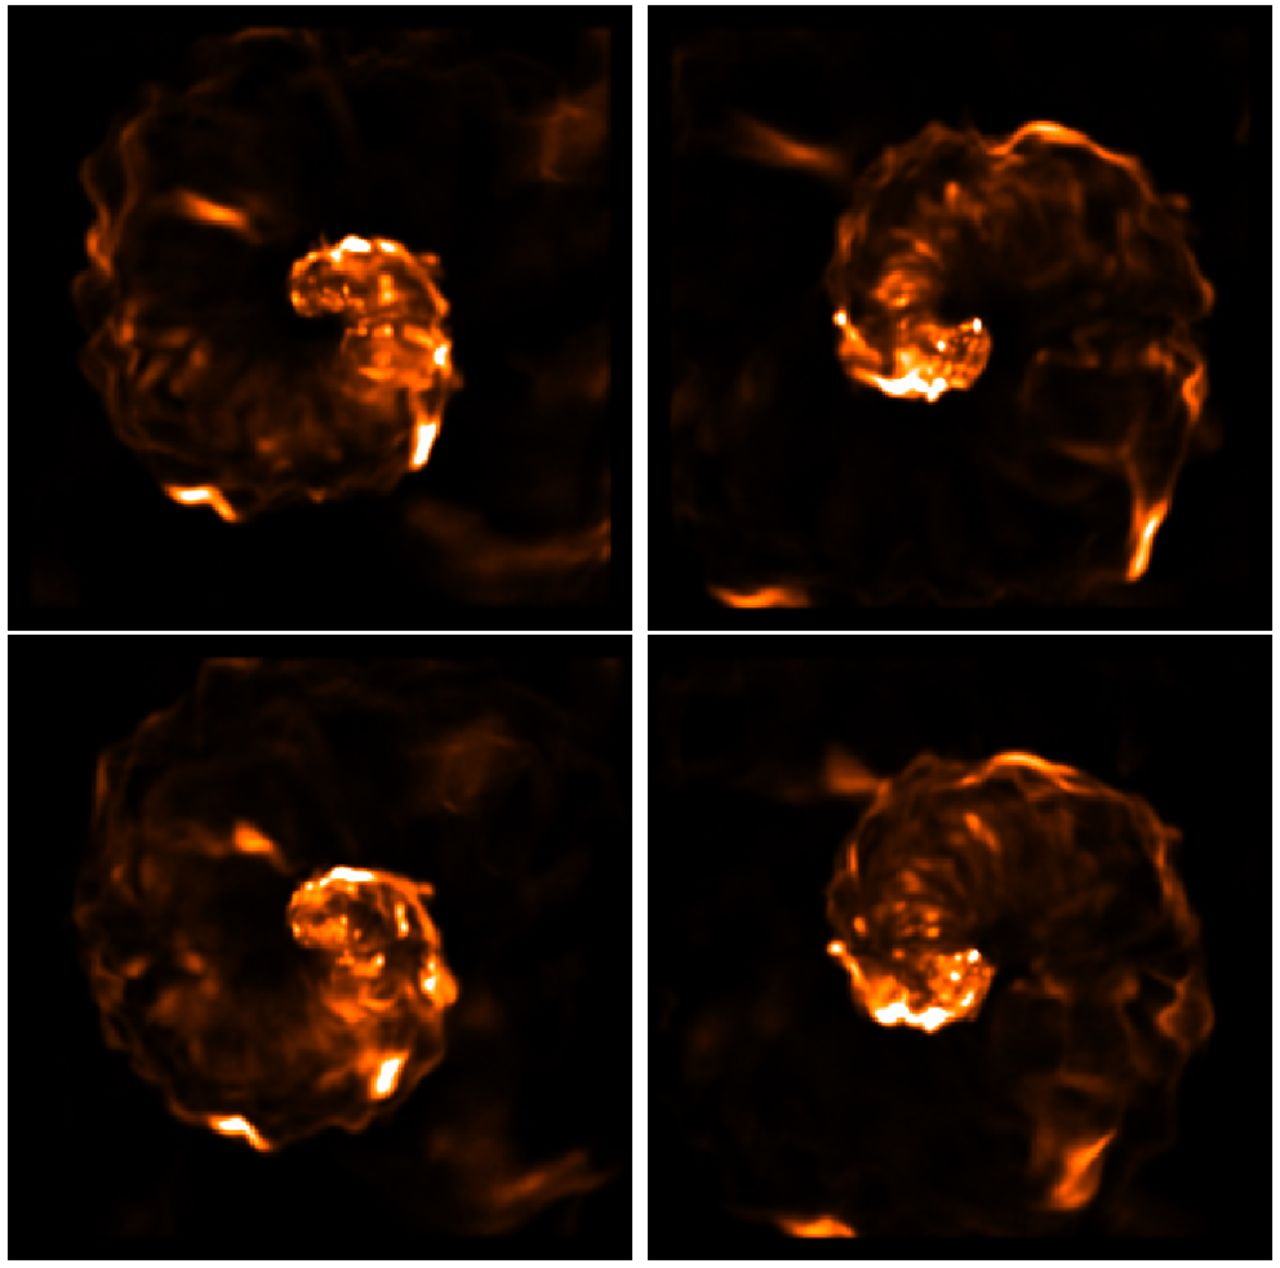
\includegraphics{assets/hendrix-synthetic-observation.jpeg}
  \caption[\textit{Radiative transfer images of WR98a \parencite{hendrix_pinwheels_2016}}]{Synthetic images of WR 98a emulating the capabilities of ALMA using a radiative transfer model, reproduced from \textcite{hendrix_pinwheels_2016}.}
  \label{fig:hendrix-synthetic}
\end{figure}

\chapter[A Parameter Space Exploration of Dust Formation]{A Parameter Space Exploration of Dust Formation within WCd Systems Using an Advected Scalar Dust Model}


\begin{abstract}
    
\end{abstract}

\section{Introduction}


Binary systems with colliding stellar winds are a fascinating phenomena capable of producing a variety of phenomena, the shock produced from these interacting systems is one of the most luminous persistent stellar-mass X-ray sources in the night sky, 
\parencite{usov_stellar_1991}, within the wind collision region the available mechanical energy rivals the radiative energy of many stars, producing shocks with temperatures exceeding $10^8$ \si{\kelvin} with densities approximately 4 orders of magnitude higher than the local medium.

Despite this, in particularly energetic Colliding Wind Binary\footnote{CWB} systems, such as those with an evolved Wolf-Rayet (in particular the WC sub-type) star as the source of the dominant wind in the system\footnote{A WR+OB binary} dust has been observed to form.
\cite{allenInfraredPhotometryNorthern1972} first attributed IR excess around WC systems to dust in the form of amorphous carbon grains; however, the high wind temperatures and extremely high luminosities around WC systems is such that dust grains would be readily destroyed through sublimation processes.
Despite this, dust has been observed to form readily in binary systems\footnote{WCd system}, even with an additional highly luminous star and a shock that would quickly destroy dust acting upon these nascent, fragile dust grains.
The exact mechanisms of dust formation as well as the evolution of dust within these systems is poorly understood, however dust formation rates can be extremely high, up to $10^{-8}$ \si{\solarmass\per\year}, or approximately $0.1\%$ of the total wind by mass.

% Persistent and episodic dust forming systems
% Discuss leading theories briefly

Dust has also been observed forming either consistently and periodically within different colliding wind binary systems.
Whilst the exact mechanism for this condition is not currently known, there is a strong correlation between periodicity and eccentricity, with more circularly orbiting systems exhibiting 
Due to this orbital dependency, it is likely that there is an optimal dust forming separation, where dust can form in large quantities. This could be due to factors such as strong post shock cooling, which is highly dependent on the wind speed and orbital separation.
Additionally, dust may be protected from the bulk of the stellar radiation due to the extremely large degree of extinction from the dense post-shock environment.

% Why is it so hard to observe these systems?

Direct observation of dust forming CWB, in particular the Wind Collision Region\footnote{WCR} is exceptionally difficult for a number of reasons:

\begin{itemize}
  \item WR+OB CWB systems are extremely rare, with $< 100$ systems having been detected within the Milky Way.
  \item Not all WC+OB systems are dust producing, limiting the sample size further.
  \item Galactic WCR systems are comparatively distant from earth, WR 104, a well-studied system, is at a distance of $\sim 2.5$ \si{\kilo\parsec}, this prevents observations of these systems at a high angular resolution.
  \item The surrounding dust cloud and high densities of the WCR introduce extreme levels of extinction, limiting visible light observations of these systems.
  \item Based on observations of CWB systems (//TODO cite this) it appears that initial grain growth is quite rapid, this means that studying the evolution of dust as it travels through the system is exceedingly difficult.
\end{itemize}

Numerical simulations, for these reasons, are ideal for modelling the growth of dust grains within this unresolved region.

% Proposal of work, what is this project covering?

In order to better understand what influences dust production in a CWB system, a parameter space exploration of the wind and orbital parameters was performed.
In particular the orbital separation, mass-loss rate and wind velocity were modified for both stars in order to influence the wind momentum ratio, $\eta$, and the cooling parameter, $\chi$.

% Discussion of parameters, eta and chi

The wind momentum ratio is a measure of the imbalance between the two winds, given as the ratio of the total wind momenta of both stars in the system:

\begin{equation}
  \eta = \frac{\dot{\text M}_\text{OB} v^\infty_\text{OB}}{\dot{\text M}_\text{WR}v^\infty_\text{WR}} ,
\end{equation}

where $\dot{\text{M}}$ is the mass loss rate of a star, while $v^\infty$ is the terminal velocity of a stars outflow.
A low value for $\eta$ indicates that the winds are extremely imbalanced, with one star dominating the wind dynamics of the system.
The wind momentum ratio can also be used to provide an approximation of the dynamics of the system, for a given orbital separation, $d_\text{sep}$ the distance from each star to the apex of the wind collision region shock can be estimated with the formulae:

\begin{subequations}
  \begin{align}
    r_\text{WR} & = \frac{1}{1+\eta^{1/2}} d_\text{sep} , \\
    r_\text{OB} & = \frac{\eta^{1/2}}{1+\eta^{1/2}} d_\text{sep} .
  \end{align}
\end{subequations}

In the case of a very small wind momentum ratio the primary stars wind completely envelopes the secondary stars forming a strong shock front; the geometry of which can be approximated in the form of a conic surface with an opening angle, $\theta$,

\begin{equation}
  \theta \simeq 2.1 \left( 1 - \frac{\eta^{2/5}}{4}\right) \eta^{-1/3} ~~~ \text{for} ~ 10^{-4} \leq \eta \leq 1 ,
\end{equation}

to a high degree of accuracy \parencite{eichler_particle_1993}.

The cooling parameter, $\chi$, compares the cooling time to the escape time from the shock region for a parcel of gas in the immediate post-shock environment. An approximation can be made using the known parameters of a system using the equation:

\begin{equation}
    \chi = \frac{t_\text{cool}}{t_\text{esc}} \approx \frac{v_8^4 d_{12}}{\dot{\text M}_{-7}} , 
\end{equation}

where $v_8$ is the wind terminal velocity in units of $10^8$ \si{cm.s^{-1}}, $d_{12}$ is the distance to the WCR apex in units of $10^{12}$ \si{cm}, and $\dot{\text M}_{-7}$ is the mass loss rate in units of $10^{-7} \si{\solarmass\per\year}$ \parencite{stevens_colliding_1992}.
Small values of $\chi$ indicate that radiative cooling dominates the dynamics of the system, while larger values indicate an adiabatic system.
Strong cooling occurs in comparatively slow, dense winds with a high metallicity, as such it can be predicted that the post-shock WR flow will rapidly cool from the immediate post-shock temperature of $10^8 \, \si{\kelvin}$ to temperatures in the dust formation range, $\lesssim 10^4 \, \si{\kelvin}$.

%//TODO Quick section on why this is important

\section{Methodology}

Numerical simulations within this paper utilise the Athena++ hydrodynamical code, a highly modular modern fluid dynamics code \parencite{stoneAthenaAdaptiveMesh2020}.
Simulations are generated in 3D and the Euler hydrodynamical equations are solved in the form:

\begin{subequations}
  \begin{align}
    \frac{\partial\rho}{\partial t}+\nabla \cdot \left(\rho \boldsymbol{u}\right) & = 0 , \\
    \frac{\partial \rho \boldsymbol{u}}{\partial t} + \nabla \cdot \left(\rho \boldsymbol{u} u + P \right) & = 0, \\
    \frac{\partial \rho \varepsilon}{\partial t} + \nabla \cdot \left[ \boldsymbol{u} \left( \rho\varepsilon + P \right) \right] & = \dot E_{cool} , 
  \end{align}
\end{subequations}

where $\varepsilon$ is the total specific energy, $\varepsilon = \boldsymbol{u}^2/2 + e/\rho $, $\rho$ is the mass density, $e$ is the internal energy density, $P$ is the gas pressure and $u$ is the gas velocity.
In order to simulate radiative losses, the parameter $\dot E_{cool}$ is included, which is the energy loss rate from the fluid due to gas and dust cooling, which is elaborated on in section \ref{sec:gas-dust-cooling}.

% Technical details

Athena++ has been configured to run using a piecewise linear reconstruction method with a 4\ts{th} order Strong Stability Preserving Runge-Kutta time-integration method \parencite{spiteriNewClassOptimal2002}.
Athena++ was forked from the original repository and additional routines were written for a Colliding Wind Binary case.
To simulate the dynamics of the simulation functions were created to produce a steady outflow from a small spherical region around a set of cartesian co-ordinates as well as a function to move these co-ordinates with each time-step; these were used to simulate stellar wind outflow orbital motion respectively.
Additionally, Athena++ was further modified to include an advected scalar dust model for simulating dust growth and destruction as well as a photon emission cooling model to approximate cooling for gas and dust particles within the fluid.
Athena++ utilises OpenMPI for parallelism, breaking the simulation into blocks, which are distributed between processors, the block size is variable, but for these simulations a block size of $32\times 32 \times 8$ was found to be optimal.
This meshblock system is also utilised in mesh refinement for increasing effective resolution.
As the CWB systems are being simulated in their entirety, a very large area needs to be simulated, while at the same time the region between the stars must be resolved with a resolution of at least 100 cells in order to adequately resolve the WCR.
This difference in length scales necessitates the use of static mesh refinement to improve the effective resolution of the simulation.
A base coarse resolution of $320 \times 320 \times 40$ cells is defined for the simulations, while a region close to the binary pair operates at a higher refinement level, resulting in a resolution increase with a factor of $2^{n-1}$ greater than the coarse resolution, where $n$ is the refinement level; this can be seen in figure \ref{fig:smr-grid} where .
this results in an effective resolution $20480 \times 20480 \times 2560$ cells.
SMR is utilised instead of Adaptive Mesh Refinement, a more flexible conditional method as it has proven to be more reliable within Athena++, as it mitigates unintentional over-refinement.
As much of the grain evolution occurs a small distance from the WCR stagnation point, much of the simulation can be run at a lower resolution without affecting the simulation outcome.

\begin{figure}
  \centering
  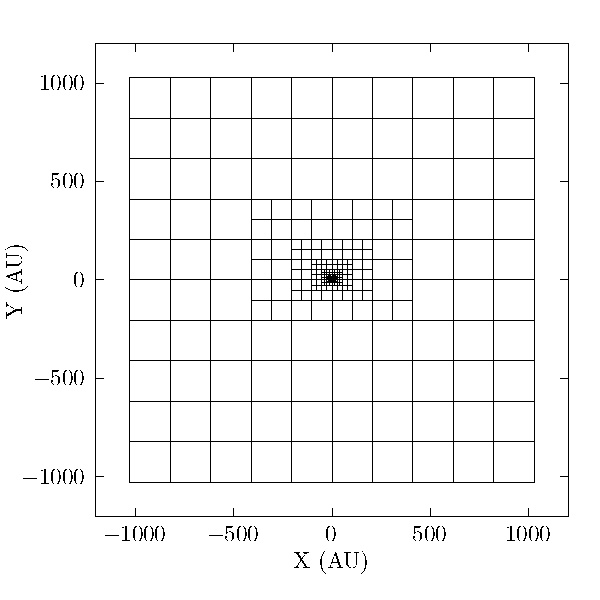
\includegraphics{assets/mesh/gridxy.pdf}
  \caption[Static mesh refinement example]{Plot of blocks used in a 7 level simulation with a block size of $32\times 32 \times 8$ cells, block density increases dramatically closer to the barycentre.}
  \label{fig:smr-grid}
\end{figure}

Wind outflow from stars is simulated by replacing the conserved values for density, momentum and energy within a small region around the expected position of the stars; this region is typically on the order of 6 maximally refined cells in radius.
This rewrite corresponds to a change in mass and mechanical energy imparted by an outflowing wind, such that:

\begin{subequations}
  \begin{align}
    \rho_R & = \frac{\dot M}{(4 \pi r^2 v_\infty)} , \\
    P_R & = \frac{\rho_R}{\mu m_H} k_B T_w , \\
    p_{R} & = \rho_R v_{R} , \\
    E_R & = \frac{P_R}{\gamma - 1} + \frac{1}{2} \rho_{R} v_{r}^2 ,
  \end{align}
\end{subequations}

% This may need more explanation, depending on previous equations

where $v_r$ is the wind velocity as it flows radially from the center of the ``remap zone'' and $r$ is the distance from the current cell to the centre of the remap zone.
Orbits are calculated by moving the remap zones in a manner consistent with Keplerian dynamics, which are updated at every timestep.

% Plasma and dust cooling

\subsection{Gas and dust cooling} \label{sec:gas-dust-cooling}

Cooling due to photon emission from gas molecules and dust particles is simulated by removing energy from a cell at each timestep.
The total energy loss is calculated by integrating the energy loss rates due to plasma and dust cooling using the Euler method; in regions with very rapid cooling sub-stepping is used to improve accuracy, with the number of sub-steps being determined by comparing the substep time to the cooling timescale of the cell.
Gas cooling is simulated using a lookup table method, a data file containing the gas temperature and associated emissivity, $\Lambda(T)$ of the wind at that temperature is read into the simulation.
In a typical cooling step, the temperature is calculated and a binary search is performed to find the nearest temperature in the lookup table, a linear interpolation step is then performed to find an appropriate value for $\Lambda$.
The emissivity is normalised for a $1 \si{cm^{-3}}$ volume with a density of $1 \si{g.cm^{-3}}$, as such, the energy loss can be calculated with the formulae:

\begin{equation}
  \frac{dE}{dt} = \left(\frac{\rho}{m_H}\right)^2 \Lambda_w(T),
\end{equation}

where $\rho$ is the gas density and $m_H$ is the mass of a hydrogen atom.
The lookup table was generated by mixing a series of cooling curves generated by MEKAL simulations of elemental gasses, these are combined based on the elemental abundances of each wind such that:

\begin{equation}
  \Lambda(T) = n_e n_i \sum{X_E \Lambda_{E}(T)},
\end{equation}

where $n_e$ and $n_i$ are the electron and ion number density of an element, $X_E$ is the abundance of an element, while $\Lambda_E(T)$ is the cooling parameter of an element.
Figure \ref{fig:cooling-curve} shows the cooling curves used for each star, as well as non-normalised emissivities for each element.
Two lookup tables are used in the simulations, based on the elemental abundances of each star. the Wolf-Rayet star uses a curve with abundances typical of a WC9 star with total hydrogen depletion and a high carbon mass fraction, while the OB star is assumed to have solar abundances.
The most significant abundances used in this projects simulations are presented in table \ref{tab:abundances}.
The cooling regime of this code ranges from $10^4$ to $10^9 \si{\kelvin}$, cooling or heating above or below these temperatures are automatically restricted.

\begin{table}
  \centering
  \begin{tabular}{@{}ccc@{}}
  \toprule
  \multicolumn{1}{l}{} & \multicolumn{2}{c}{X(E)} \\ \cmidrule(l){2-3} 
   & Solar & WC9 \\ \midrule
  H & $0.705$ & $0.0$ \\
  He & $0.275$ & $0.546$ \\
  C & $3.07 \times 10^{-3}$ & $0.4$ \\
  N & $1.11 \times 10^{-3}$ & $0.0$ \\
  O & $9.60 \times 10^{-3}$ & $0.05$ \\
  % Ne & $1.75 \times 10^{-3}$ & $0.0$ \\
  % Na & $3.47 \times 10^{-5}$ & $3.47 \times 10^{-5}$ \\
  % Mg & $7.10 \times 10^{-4}$ & $7.10 \times 10^{-4}$ \\
  % Al & $6.13 \times 10^{-5}$ & $6.13 \times 10^{-5}$ \\
  % Si & $8.60 \times 10^{-4}$ & $8.60 \times 10^{-4}$ \\
  % S & $3.82 \times 10^{-4}$ & $3.82 \times 10^{-4}$ \\
  % Ar & $1.01 \times 10^{-4}$ & $1.01 \times 10^{-4}$ \\
  % Ca & $6.15 \times 10^{-5}$ & $6.15 \times 10^{-5}$ \\
  % Fe & $1.52 \times 10^{-3}$ & $1.52 \times 10^{-3}$ \\
  % Ni & $7.65 \times 10^{-5}$ & $7.65 \times 10^{-5}$ \\ \bottomrule
  \end{tabular}
  \caption[Abundances used for OB and WR stars]{Abundances used for OB and WR stars, other elements are effectively trace.}
  \label{tab:abundances}
\end{table}


\begin{figure}[ht]
  \centering
  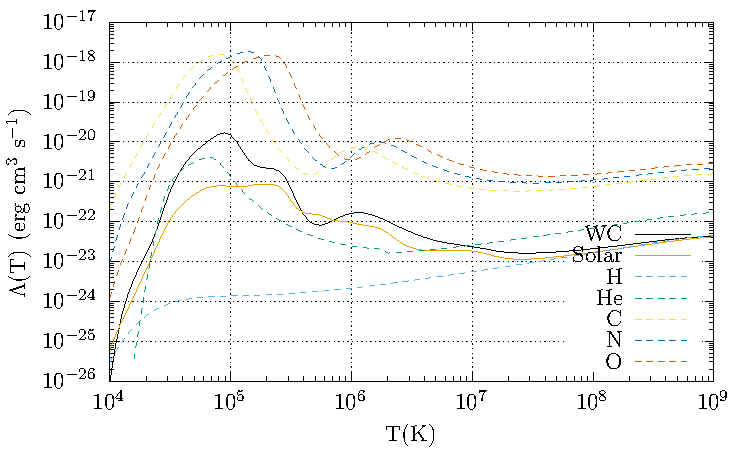
\includegraphics{assets/cooling-curve/cooling-curve.pdf}
  \caption[WR and OB $\Lambda(T)$ cooling curves]{Comparison of lookup tables for calculating energy loss due to gas cooling, pure elemental cooling curves from MEKAL have been provided for the more abundant elements.}
  \label{fig:cooling-curve}
\end{figure}

A model for cooling due to emission from dust grains is also included as dust cooling was expected to play a significant role in the evolution of each system.
The rate of cooling is calculated using the uncharged particle case of the Dwek \& Werner prescription \parencite{dwek_infrared_1981}.
Grains are heated due to collisions with ions and electrons, causing them to radiate, with energy being removed from the simulation.
This assumes that infrared emission due to collisional heating is shorter than the cooling timestep, and the region being simulated is optically thin to far infrared photons.
Ions are calculated by element by estimating their number density, with the energy loss rate calculated with the following formulae:

\begin{subequations}
  \begin{align}
    H_\text{coll} & = 1.26 \times 10^{-19} \frac{n}{A^{1/2}} a^2(\mu \text m) T^{3/2} h(a,T) , \\
        \Lambda_d & = \frac{H_\text{coll} + H_\text{el}}{n_H} , \\
    \frac{dE}{dt} & = n_T n_d \Lambda_d ,
  \end{align}
\end{subequations}

where $H_\text{coll}$ is the heating rate due to atom and ion collisions, $H_\text{el}$ is the heating rate due to electron collisions, $h(a,T)$ is the grain-ion transparency and $n_T$ is the total number density.
$H_\text{coll}$ is summated for Hydrogen, Helium, Carbon, Nitrogen and Oxygen atom collisions, other elements are not considered as they are present in trivial proportions in both winds.

Electron-grain collisions are modelled similarly to ions, albeit with some differences.
One major factor for calculating accurate energy loss due to electron collisions is that the electron number density needs to be accurately calculated; this is performed with a second series of lookup tables that contain the electron-to-ion ratio of each wind across a temperature range of $10^4$ to $10^9\si{\kelvin}$ (figure \ref{fig:electron-curve}).
The electron number density is found to be $n_e = n_e/n_i n_i$ where $n_e/n_i$ is the electron-to-ion ratio and $n_i$ is the ion number density.

\begin{figure}[h]
  \centering
  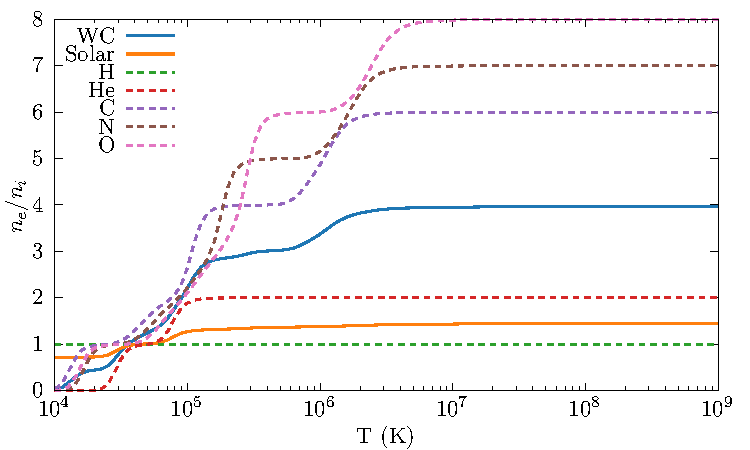
\includegraphics{assets/ionisation-fraction/ionisation-fraction.pdf}
  \caption[OB and WR electron-ion ratios]{A comparison of the electron-ion ratio of both winds as temperature changes, included are the pure wind flows that the lookup tables are built from.}
  \label{fig:electron-curve}
\end{figure}

Additionally, calculating electron-grain transparency is a significantly more complex problem than calculating ion-grain transparency.
Electron-grain transparency is calculated via an approximation described in Dwek \& Werner:

\begin{equation}
  \begin{alignedat}{3}
    h(x^*) & = 1 ,                && ~~ x^* > 4.5, \\
           & = 0.37{x^*}^{0.62} , && ~~ x^* > 1.5 , \\
           & = 0.27{x^*}^{1.50} , && ~~ \text{otherwise,}
  \end{alignedat}
\end{equation}

where $x^* = 2.71\times 10^8 a^{2/3} (\si{\micro\metre})/T$.
This approximation is approximately 4 orders of magnitude faster than using an integration method, while only being out by $\sim 8\%$ in the worst case scenario (figure \ref{fig:lambdacomparison}).

\begin{figure}
  \centering
  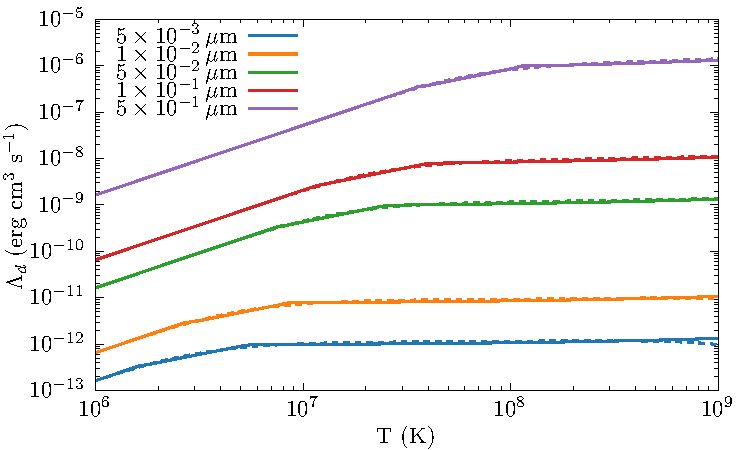
\includegraphics{assets/grain-transparency/lambda-comp.pdf}
  \caption[Comparison of electron transparency methods.]{$\Lambda_d$ as a function of temperature for various grain sizes, the estimate method is extremely close to the integral value aside from at the highest temperatures.}
  \label{fig:lambdacomparison}
\end{figure}

%//TODO this caption is the same as another one, need to come up with a new one!

Grain-grain collision is not modelled, as this would be difficult to calculate due to the single-fluid model in use, further simulations utilising a multi-fluid model could allow for this to be simulated.

% Advected scalar modification

\subsection{Numerical modelling of dust through advected scalars}

The most important modification for Athena++ was the addition of a dust growth and destruction model to simulate the production of dust within the WCR.
A passive scalar model was used where which dust can evolve and advect through the simulation, analogous to a co-moving fluid, which previous papers have noted is an accurate dynamical model for dust within the WCR \parencite{hendrix_pinwheels_2016}.
In these simulations, dust is stored in the form of two variables, the average grain radius, $a$, and the dust-to-gas mass ratio, $z$.
From these constants the dust production rate, number density, and total dust mass can be derived.
A co-moving model allows for a simplified model of dust formation. In such a model, the mean particle velocity between two particles of different size can be given as:

\begin{equation}
  \langle u \rangle = \left[ \frac{8kT}{\pi m_r} \right] ^{1/2} ,
\end{equation}

where $m_r$ is the familiar reduced mass between a test particle of mass $m_t$ and a field particle of mass $m_f$

\begin{equation}
  m_r = \frac{m_f m_t}{m_f + m_t} .
\end{equation}

As the dust grain is significantly more massive, the reduced mass is approximately equal to the grain mass, simplifying the dynamics of the simulation in a co-moving case \parencite{spitzer_jr._physical_2008}.
Dust growth is modelled through approximating growth due to grain-gas accretion, grains co-moving with a gas perform low-velocity\footnote{Relative to the overall wind velocity} collisions with the surrounding gas, accreting this gas onto the surface of the dust grain \parencite{spitzer_jr._physical_2008}.
Assuming a single average grain size and a relatively consistent grain number density the change in average grain radius and total dust mass density can be described in the form:

\begin{subequations}
  \begin{align}
        \frac{da}{dt} & = \frac{\xi_a \rho_{Gr} w_a}{4 \rho} , \\
    \frac{\rho_D}{dt} & = 4 \pi a^2 \rho n_D \frac{da}{dt}   , 
  \end{align}
\end{subequations}

where $w_a$ is the Maxwell-Boltzmann distribution RMS velocity, $\xi_a$ is the grain sticking efficiency, $\rho_{Gr}$ is the grain bulk density, $\rho$ is the gas density, $a$ is the dust grain radius, and $n_D$ is the grain number density.
In this paper $\xi_a$ is assumed to be $10\%$, while a bulk density analogous to amorphous carbon grains of $3.0 \, \si{g.cm^{-3}}$ is utilised.
Additionally, dust destruction is calculated via gas-grain sputtering using the Draine \& Salpeter prescription - a dust grain has a lifespan, $\tau$, which is dependent on the grain radius, as the grain loses radius proportional to its loss in mass; assuming a spherical grain, the rate of change in mass and radius can be calculated such that:

\begin{subequations}
  \begin{align}
           \tau_D & = 1 \, \text{Myr} \times \frac{a}{n_g} , \\
    \frac{da}{dt} & = - \frac{a}{\tau_D} , \\
    \frac{dm}{dt} & = -1.33 \times 10^{-13} a^2 n_g n_d \rho_{Gr} ,
  \end{align}
\end{subequations}

where $n_g$ is the gas number density \parencite{draine_destruction_1979}.

% //TODO cleanup sentence structures

In order to propagate dust through each simulation, a small initial value for the advected scalars is set in each cell in the remap zones, a minimum grain radius of $50 \, \text{\AA}$ and minimum dust-to-gas mass ratio of $10^{-8}$ is proposed.
Changing $z_{min}$ does not significantly impact the average final dust-to-gas mass ratio of the system as $z$ rapidly increases within the WCR, and only impacts the amount of dust formed outside of the WCR.

\section{Model Parameters}

For this paper, a series of simulations were run in order to determine how dust formation varies due changes in orbital separation and wind momentum ratio.
A baseline simulation with properties similar to WR98a but with simplified orbits was created, which was then modified to influence the orbital separation and wind momentum ratio.
Another set of simulations were run where the cooling mechanisms were selectively disabled, in order to understand how 
Table \ref{tab:baseline-windproperties} and \ref{tab:baseline-orbits} detail the wind and orbital parameters of the baseline simulation.
Orbital separation is modified by changing the orbital period of the simulation, while wind momentum ratio is modified by adjusting the mass loss ratio and wind terminal velocity for each star.

\begin{table}[h]
  \centering
  \begin{tabular}{cccc}
  \hline
  Parameter & WR & OB & Unit \\ \hline
  $\dot M$ & \num{5.0e-6} & \num{5.0e-8} & \si{\solarmass\per\year} \\
  $v_\infty$ & \num{1e8} & \num{2e8} & \si{cm.s^{-1}} \\
  $T_w$ & \num{1e4} & \num{1e4} & K \\
  \hline
  \end{tabular}
  \caption{Wind properties of the baseline system}
  \label{tab:baseline-windproperties}
\end{table}

\begin{table}[h]
  \centering
  \begin{tabular}{ccc}
  \hline
  Parameter & Value & Unit \\ \hline
  $M$ & 10.0 & \si{\solarmass} \\
  $d_{sep}$ & \num{5.984e13} & cm \\
  $P$ & \num{5.64e7} & s \\
  \hline
  \end{tabular}
  \caption{Baseline system orbital properties}
  \label{tab:baseline-orbits}
\end{table}

\subsection{Cooling mechanisms}

For this set of simulations, the influence of cooling was changed by varying how cooling works within the simulations.
All simulations in this set do not vary their orbital or wind parameters, which are that of the baseline system described in tables \ref{tab:baseline-windproperties} \& \ref{tab:baseline-orbits}, the main differing factor between simulations is the avenues available for cooling, the main simulation has both plasma and dust cooling in operation, while the other two simulations have plasma cooling only and no cooling respectively (table \ref{tab:cooling-param}).
The final, no radiative cooling simulation instead relies on adiabatic expansion for temperature change; as such, this simulation behaves as if it has a $\chi$ value for both winds that is arbitrarily high.
These simulations were performed in order to test the temperature response of the dust model, to ensure the stability of the cooling models, and to determine the role of cooling itself in the formation of dust.

% Discuss why this is important, mention overdensity due to radiative cooling

\begin{table}[h]
  \centering
  \begin{tabular}{ccc}
    \hline
    Name & Plasma cooling & Dust cooling \\
    \hline
    \texttt{fullcool} & Yes & Yes \\ 
    \texttt{plasmacool} & Yes & No \\
    \texttt{nocool} & No & No \\
    \hline
  \end{tabular}
  \caption{Cooling series simulation parameters}
  \label{tab:cooling-param}
\end{table}

\subsection{Wind momentum ratio}

A second set of simulations were devised in order to determine the role $\eta$ has on the formation of dust.
These simulations have similar orbital properties to the baseline simulation, but with varying wind properties.
$\eta$ is varied from 0.01 to 0.04 by adjusting the wind parameters for each star, this experiment is further subdivided by which property is modified, either the mass loss rate or wind terminal velocity.
Multiple simulations have similar momentum ratios and cooling parameters, but accomplished via different means, such as changing the secondary star wind rather than the primary. This is done in order to determine whether dust production changes are due to these two parameters or to the momentum ratio itself.
These simulations are also compared to the baseline simulation, which has a momentum ratio of 0.02.
These simulations were run out to a minimum of 1 orbit, with some simulations run out further to rule out the role of orbital position and simulation advection, as the results should be consistent across multiple orbits. 

\begin{table}[h]
  \centering
  \begin{tabular}{ccccccc}
  \hline
  Name & $\dot M_{WR}$ & $\dot M_{OB}$ & $v^\infty_{WR}$ & $v^\infty_{OB}$ & $\eta$ & $\chi_{WR}$ \\ 
  & \si{\solarmass\per\year} & \si{\solarmass\per\year} & \si{\centi\metre\per\second} & \si{\centi\metre\per\second} & & \\ \hline
  \texttt{baseline}& \num{5.0e-6} & \num{5.0e-8} & \num{1e8} & \num{2e8} & 0.02 & 1.049 \\
  \texttt{mdot-1}& \num{1.0e-5} & \num{5.0e-8} & \num{1e8} & \num{2e8} & 0.01 & 0.544 \\
  \texttt{mdot-2}& \num{2.5e-6} & \num{5.0e-8} & \num{1e8} & \num{2e8} & 0.04 & 1.995 \\
  \texttt{mdot-3}& \num{5.0e-6} & \num{1.0e-7} & \num{1e8} & \num{2e8} & 0.04 & 0.997 \\
  \texttt{mdot-4}& \num{5.0e-6} & \num{2.5e-8} & \num{1e8} & \num{2e8} & 0.01 & 1.088 \\
  \hline
  \end{tabular}
  \caption[Mass loss rate series wind parameters]{Wind parameters for simulations varying the mass loss rate, $\dot M$.}
  \label{tab:mdot-param}
\end{table}

\begin{table}[h]
  \centering
  \begin{tabular}{ccccccc}
  \hline
  Name & $\dot M_{WR}$ & $\dot M_{OB}$ & $v^\infty_{WR}$ & $v^\infty_{OB}$ & $\eta$ & $\chi_{WR}$ \\ 
  & \si{\solarmass\per\year} & \si{\solarmass\per\year} & \si{\centi\metre\per\second} & \si{\centi\metre\per\second} & & \\ \hline
  \texttt{baseline} & \num{5e-6} & \num{5e-8} & \num{1e8} & \num{2e8} & 0.02 & 1.049 \\
  \texttt{vinf-1} & \num{5e-6} & \num{5e-8} & \num{2e8} & \num{2e8} & 0.01 & 17.41 \\
  \texttt{vinf-2} & \num{5e-6} & \num{5e-8} & \num{5e7} & \num{2e8} & 0.04 & 0.062 \\
  \texttt{vinf-3} & \num{5e-6} & \num{5e-8} & \num{1e8} & \num{4e8} & 0.04 & 0.997 \\
  \texttt{vinf-4} & \num{5e-6} & \num{5e-8} & \num{1e8} & \num{1e8} & 0.01 & 1.088 \\
  \hline
  \end{tabular}
  \caption[Terminal velocity series wind parameters]{Wind parameters for simulations varying the wind terminal velocity, $v^\infty$.}
  \label{tab:vinf-param}
\end{table}

\subsection{Separation distance}

A final series of simulations was performed with a binary pair utilising wind parameters described in table \ref{tab:baseline-windproperties} with a differing orbital separation. Separation was modified by changing the orbital period of each star; in this series, orbital separation was varied from \SI{4}{\au} to \SI{64}{\au} (table \ref{tab:dsep-param}). The main effect of adjusting the orbital radius is the subsequent modification of the cooling parameter, $\chi$, which is inversely proportional to the separation distance. As such, the purpose of these simulations is to confirm that dust formation rate relies strongly on $\chi$, or if there are other factors involved in dust formation. %//TODO clean up

Each simulation has a coarse resolution of $320 \times 320 \times 40$ cells, with a varying number of levels, as the separation distance is doubled, the associated static mesh refinement box is halved and the number of levels is decremented. This manipulation of levels ensures that the number of cells between the stars is kept consistent, reduces memory usage and keeps the average timestep approximately the same.
Similarly to the previous set of simulations, a minimum of 1 orbit was needed for each simulation, however, as the orbital period of each simulation varies, certain simulations were able to run for a significantly longer length of time, with data for multiple orbits being obtained.

%//TODO calculate the chi in each simulation
\begin{table}[h]
  \centering
  \begin{tabular}{cccccc}
    \hline
    Name & P & $d_{sep}$ & $\chi_{WR}$ & Levels & Effective Resolution \\
    & \si{\second} & \si{\au} &  &  & Cells \\ \hline 
    \texttt{dsep-4AU} & \num{5.647e7} & 4  & 1.049 & 7 & $20480 \times 20480 \times 2560$ \\
    \texttt{dsep-8AU} & \num{1.597e8} & 8  & 2.097 & 6 & $10240 \times 10240 \times 1280$ \\
    \texttt{dsep-16AU} & \num{4.518e8} & 16 & 4.194 & 5 & $5120 \times 5120 \times 640$    \\
    \texttt{dsep-32AU} & \num{1.278e9} & 32 & 8.388 & 4 & $2560 \times 2560 \times 320$    \\
    \texttt{dsep-64AU} & \num{3.614e9} & 64 & 16.78 & 3 & $1280 \times 1280 \times 160$    \\ \hline
  \end{tabular}
  \caption{Parameters of simulations varying separation distance.}
  \label{tab:dsep-param}
\end{table}

\subsection{Data collection}

Data was collected in multiple forms, regular HDF5 files were generated at regular time intervals, 3D HDF5 meshes were generated every $1/100^{\text{th}}$ of an orbit, while 2D slices were produced every $1/1000^{th}$ of an orbit.
These HDF5 files contain the primitive variables of the simulation, gas density, $\rho$, gas pressure, $P$ and wind velocity components, $v_x$, $v_y$ and $v_z$; these can be used to derive other variables such as 
In addition to HDF5 outputs, history data was collected in order to plot the time evolution of the simulation, history files are log files taken at various intervals containing the volume-weighted summations of all system parameters, such as the total system mass and summated average grain radius.
In order to derive average values, such as $\bar{z}$ and $\bar{a}$ the values for each can be divided by the total system mass.
To calculate dust formation within the wind collision region, a method of determining if a cell was a part of the wind collision region was devised - the cells density would be compared to the predicted density of a single smooth wind with the wind parameters of the Wolf-Rayet star in the system:

\begin{equation}
  \rho_\text{SW} = \frac{\dot{M}_{WR}}{4 \pi r^2 v^\infty_{WR}},
\end{equation}

where $r$ is the distance from the barycentre. This threshold value was set to $1.25\rho_\text{SW}$ as it most accurately determined if a cell was part of the WCR, increased threshold values were not successful at a larger distance from the barycentre (figure \ref{fig:overdensity-threshold}), while other methods such as determining wind mixing levels were not successful in general.

\begin{figure}
  \centering
  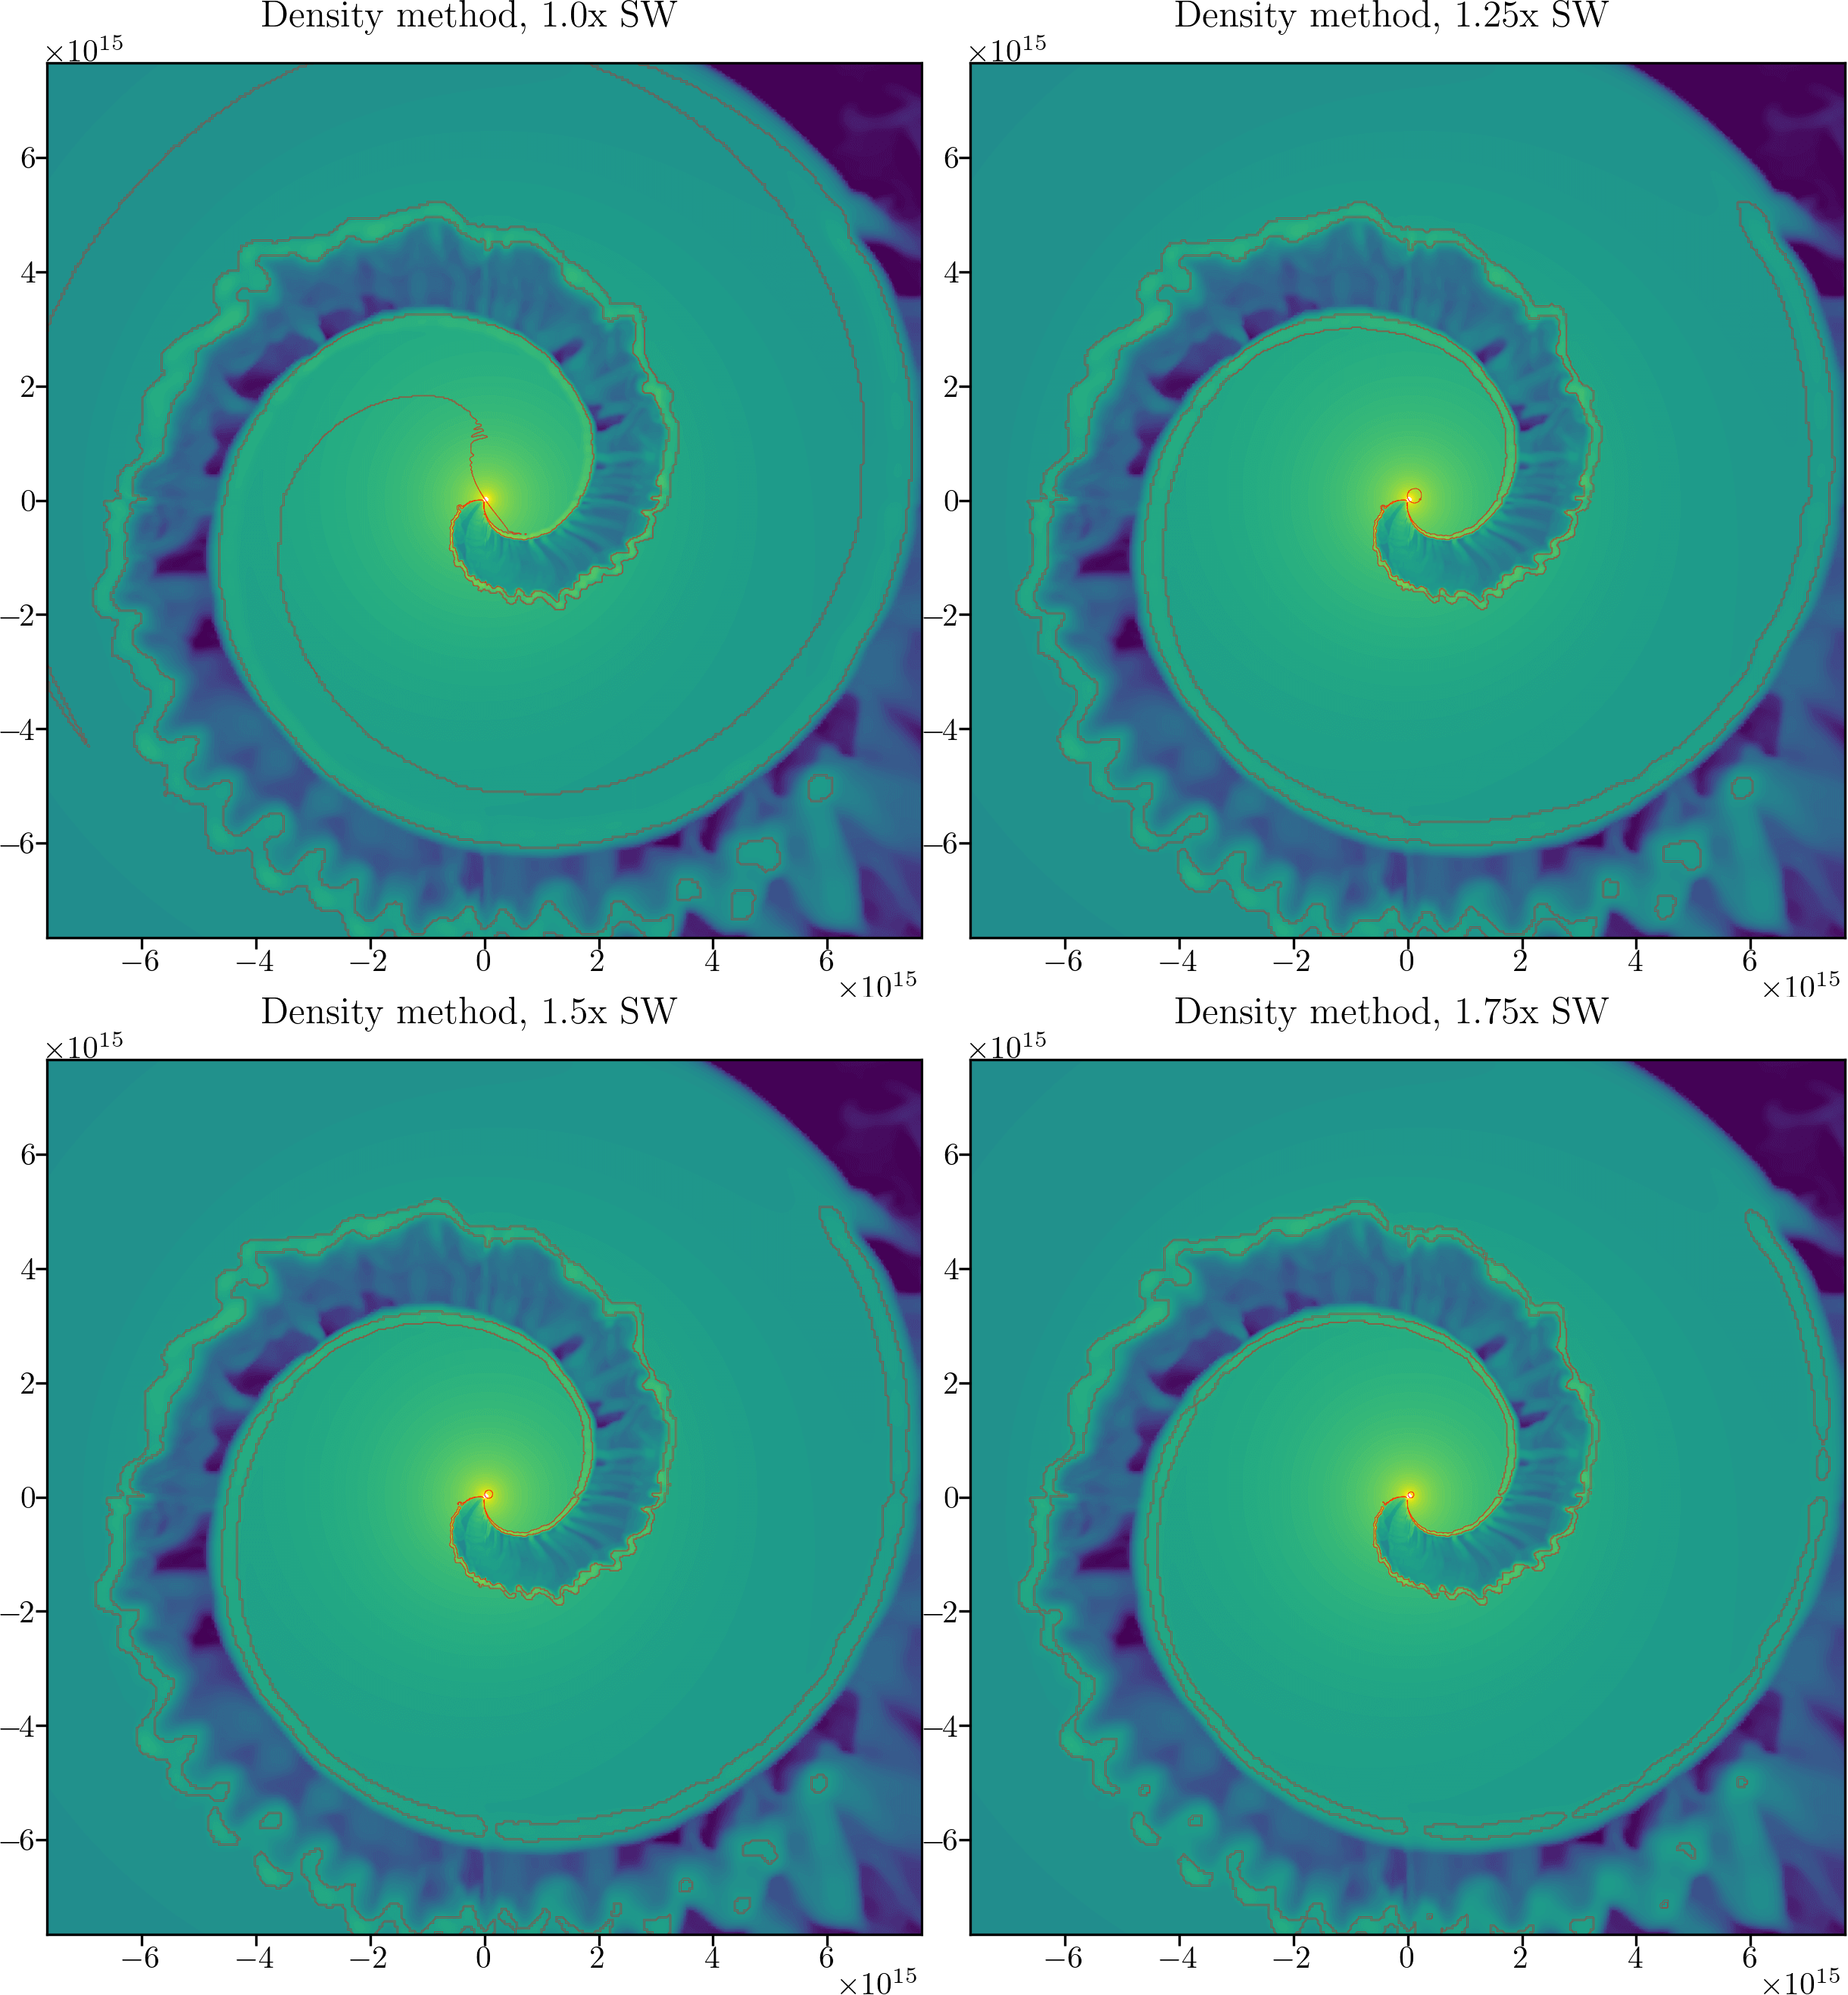
\includegraphics[width=5in]{assets/overdensity-method.png}
  \caption[Comparison of threshold values for over-density method]{Comparison of threshold values for over-density method of determining of a cell resides in the wind collision region, a threshold value of $1.25\rho_\text{SW}$ was chosen as it most accurately determined if the cell was in the post-shock region.}
  \label{fig:overdensity-threshold}
\end{figure}

\section{Results}

\subsection{Radiative processes}

\subsection{Momentum ratio variation}

\subsection{Separation variation}

% Adiabatic flow 

The most immediately apparent result to this 

%//FIXME this needs work! 32AU result is instead labelled as 64AU and zooms aren't consistent!

\begin{figure}
  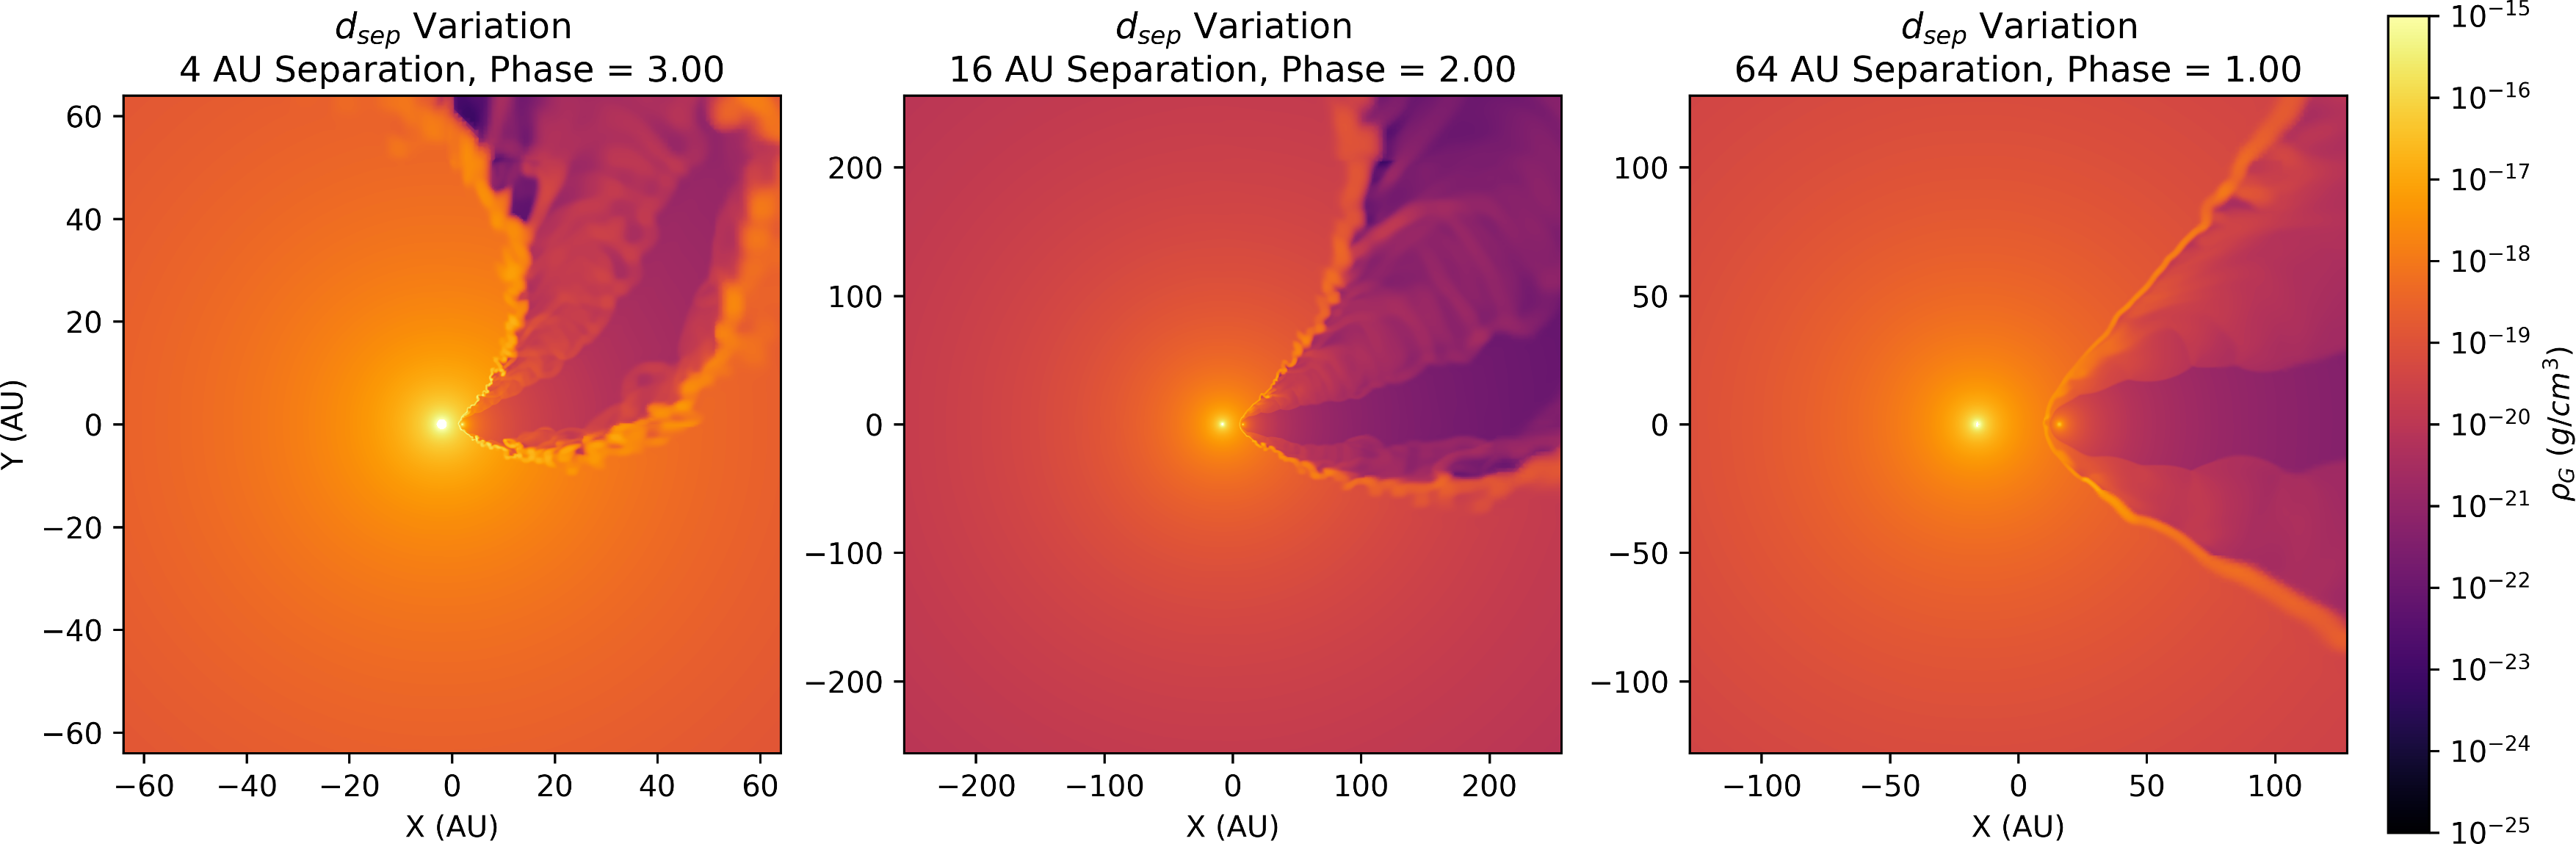
\includegraphics[width=\textwidth]{assets/adiabatic-flow/adiabatic-flow-a4.png}
\end{figure}

% Dust yields

A clear trend with orbital separation is that dust formation increases drastically as the stars are positioned closer together, at high degrees of separation dust formation ceases, and average grain size drops below the initial value of $50 \text \AA$.

The bulk of dust growth occurs in the immediate post shock region, as dust is rapidly cooled and at a high enough density for dust formation to occur.

This matches observations of episodic dust forming systems, where infrared emission due to dust is maximised at or shortly after periastron passage. This also lends further evidence that dust formation rates are not influenced solely by the momentum ratio, as this is kept constant, and instead is strongly influenced by the wind density at collision and post-shock cooling. 

% Periodicity

Closer orbits were also observed to cause subtle periodic changes, whilst this effect is less pronounced than in a highly eccentric system, the 


\subsection{Wind mixing within the WCR}

%This may need additional work

While interaction between Hydrogen and dust grains is not simulated by the dust model, \cite{leteuffModelDustFormation2002} notes that Hydrogen could be a potential catalyst for amorphous carbon grain formation.


% \appendix
% \section{Derivation of Dust Accretion and Destruction Rates}\label{app:accretiondestruction}

% \subsection{Dust destruction}\label{app:destruction}

\chapter[Exploring Dust Growth in WR140]{\secondpapertitle}
\label{ch:wr140}

\section{Introduction}

The dynamics of massive stars in binary systems is a particularly fascinating subject.
These incredibly violent phenomena are obscured behind vast clouds of outflowing stellar wind, the result of the most massive stars we know slowly tearing themselves asunder.
% Observational history, define acronyms commonly used
Colliding wind binary (CWB) systems were first hypothesised to explain highly luminous and variable x-ray emission in systems such as V444 Cyg and $\gamma^2$ Vel \parencite{prilutskii_x_1976}.
These extremely bright emissions were found to be due to stellar wind collision with shock velocities in the order of $10^3 \, \si{\kilo\metre\per\second}$.
The variability in x-ray emission can be explained if the phenomena occurs due to the orbit of a binary system, such as the Wind Collision Region (WCR) being occluded by the outflowing stellar wind, being occluded by the stars themselves.
The system can also have an eccentric orbit, reducing the shock strength as the orbital separation, $d\rms{sep}$, varies.
Despite this dust-hostile environment, CWB systems containing a Wolf-Rayet carbon phase star (WC) have been observed producing copious quantities of dust (so-called WCd systems).
These systems typically convert around $1\%$ of the stellar wind into dust a short time after wind collision; in more prolific systems such as WR104 up to $36\%$ of the Wolf-Rayet (WR) outflow is converted into dust \parencite{lauRevisitingImpactDust2020}.
This corresponds to dust production rates on the order of $10^{-6} \, \si{\solarmass\per\year}$, rivalling other profuse dust producing phenomena such as AGB stars.

WCd systems can sub-categorised further, into persistent, variable and episodic dust forming systems.
Persistent systems, such as WR104 \parencite{tuthill_dusty_1999}, produce dust at a constant rate, and as such produce extreme quantities of dust, as well as well-defined pinwheel patterns if the system is viewed face-on.
Episodic systems, meanwhile, only produce dust for a limited period before entering a period of dormancy; this pattern is cyclical, and is predictably periodic.
A good example of such an episodic system is WR140, the subject of this paper \parencite{williamsMultifrequencyVariationsWolfrayet1990}.
Variable systems have some characteristics of these two sub-types, having a distinct variability without a period of dust producing dormancy, such as WR98a \parencite{monnierPinwheelNebulaWR1999}.
Whether a system is persistent, variable or episodic is based on the systems orbital eccentricity, highly eccentric systems appear to form episodic systems, with the ``active'' dust production period occurring immediately after periastron passage, and a relatively short time thereafter.
Meanwhile, persistent and variable systems have been observed to have more circular orbits, suggesting that the effect of a change in system separation distance, $d\rms{sep}$, has a role in dust formation.
The initial mechanism behind dust formation is not well understood, whilst nascent amorphous carbon dust grain cores can form condense within the photosphere of WC7-9 stars,
%%//TODO CITE THIS 
these grain cores would be vaporised by UV flux of both stars.
However, within the WCR these grains appear to flourish, observations of these systems show that infrared excess in wavelengths associated with amorphous grains is detected almost exclusively within the post-shock WCR \parencite{soulainSPHEREViewWolfRayet2018}.
% Dust forms close to system
Observations also indicate that dust formation occurs rapidly and close to the system, this requires strong radiative cooling for the immediate-post shock temperature to reduce from $\sim 10^8 \, \si{\kelvin}$ to $\sim 10^4 \, \si{\kelvin}$
\parencite{williamsInfraredPhotometryLatetype1987,williamsMultifrequencyVariationsWolfrayet1990}.
% Bringing it all together, theories as to how dust formation occurs, density, shielding etc.
As such, dust formation appears to be encouraged in the WCR through a multitude of factors:


\begin{itemize}
  \item The high density of the post-shock WCR results in a high collision rate between carbon atoms and dust grains.
  \item The WCR shields nascent dust grains from the bulk of the UV emission from the stars.
  \item The rapid cooling in the immediate post-shock environment reduces gas-grain sputtering.
  \item Strong radiative cooling drives the formation of thermal instabilities, which produces clumps of cool, high density gas where dust can rapidly grow.
\end{itemize}

\noindent
This dust formation can also be influenced by orbital separation, velocity shear and momentum ratio imbalance between the winds, producing variability on the timescale of a single orbit, or $t\rms{dyn} \ll P$.

\begin{table}
  \centering
  \begin{tabular}{lllllll}
    \hline
    & \multicolumn{2}{c}{Persistent} & \multicolumn{2}{c}{Variable} & \multicolumn{2}{c}{Episodic} \\ \cline{2-7} 
    & Total & Example & Total & Example & Total & Example \\ \hline
   WC4 & 1 & WR19 & 0 & --- & 0 & --- \\
   WC5 & 0 & --- & 0 & --- & 1 & WR47C \\
   WC6 & 1 & WR124-10 & 0 & --- & 0 & --- \\
   WC7 & 3 & WR102-22 & 0 & --- & 4 & WR140 \\
   WC8 & 6 & WR13 & 1 & WR48a & 3 & WR122-14 \\
   WC9 & 45 & WR104 & 6 & WR98a & 1 & WR75-11 \\ \hline
   Total & 56 &  & 7 &  & 9 &  \\ \hline
  \end{tabular}
  \caption[Number of confirmed WCd systems]{Number of WCd systems with a known spectral type and dust formation type from the Galactic Wolf Rayet Catalogue \parencite{rossloweSpatialDistributionGalactic2015}. Systems with uncertain spectral types not included, while systems labelled ``d'' are included within the ``persistent'' category for their associated spectral type.}
  \label{tab:p2-wc-summated-list}
\end{table}

% Why not observe?
WCd systems are comparatively rare, out of 106 confirmed systems with a WR binary, only 9 are categorised as episodic WCd systems
(Table \ref{tab:p2-wc-summated-list}).
As these systems have a typical distance on the order of $1-10 \, \si{\kilo\parsec}$, this makes observation of WCds difficult.
Whilst these systems can be observed and the dusty WCR can be resolved, observation of the innermost, immediate post-shock dust forming region is not possible at this distance.
As such, numerical simulation is necessary to determine dust formation in WCd systems, a contemporary example of such simulations is \textcite{hendrix_pinwheels_2016}, though simulation of the evolution of dust grains through cooling, growth and sputtering was not performed.
% What we intend to do in this project
In this paper we present a numerical simulation of the archetypical episodic WCd system WR140 with a co-moving dust model simulating grain growth and sputtering through gas-grain collisions.
This simulation covers a temporal slice of the orbit of WR140 from phase $\Phi = 0.95$ to $\Phi = 1.10$, or the period immediately prior to and after periastron passage.
We will discuss our methodology in Section \ref{sec:paper-2-methodology}, with a particular emphasis on our dust model in Subsection \ref{sec:dust-model}.
Afterwards we will discuss the simulation and WR140 system parameters, as well as our data collection techniques in Section \ref{sec:paper2-wr140}.
Finally, we will discuss our results and conclude in Sections \ref{sec:p2-results} and \ref{sec:p2-conclusion}.


\section{Methodology}
\label{sec:paper-2-methodology}

The periodic dust forming system WR140 was simulated using a fork of the Athena++ hydrodynamical code \parencite{stoneAthenaAdaptiveMesh2020}, a series of modifications were implemented to simulate binary system orbits, stellar wind outflows and dust evolution.
These simulations were conducted in 3D in a Cartesian co-ordinate system.
The code solves a Riemann problem at each cell interface to determine the time-averaged values at the zone interfaces, and then solves the equations of hydrodynamics:

\begin{subequations}
  \begin{align}
    \frac{\partial\rho}{\partial t} & +\nabla \cdot \left(\rho \boldsymbol{u}\right) = 0 , \\
    \frac{\partial \rho \boldsymbol{u}}{\partial t} & + \nabla \cdot \left(\rho \boldsymbol{u} u + P \right) = 0, \\
    \frac{\partial \rho \varepsilon}{\partial t} & + \nabla \cdot \left[ \boldsymbol{u} \left( \rho\varepsilon + P \right) \right] = \frac{dE\rms{cool}}{dt} , 
  \end{align}
\end{subequations}

\noindent
where $\varepsilon$ is the total specific energy ($\varepsilon = \boldsymbol{u}^2/2 + e/\rho $), $\rho$ is the gas density, $e$ is the internal energy density, $P$ is the gas pressure and $u$ is the gas velocity.
In order to simulate radiative losses, the parameter $dE_\text{cool}/dt$ is included, which is the rate of energy loss rate per unit volume from the fluid due to gas and dust cooling.

Spatial reconstruction using a piecewise linear method was performed, while two strong stability Runge-Kutta methods were used for numerical integration, depending on the simulation stability.
Several passive scalars are utilised to model wind mixing and dust evolution, the scalar values are transported by the fluid.
For a given scalar species $i$, the scalar is advected through the scalar through the following equation:

\begin{equation}
  \rho \frac{dC_i}{dt} = \frac{\partial}{\partial t} \left( \rho C_i \right) + \nabla \cdot \left( C_i \rho \mathbf{u} \right) = -\nabla \cdot \mathbf{Q}_i ,  
\end{equation}

\noindent
where $\mathbf{Q}_i$ is the diffusive flux density ($\mathbf{Q}_i = - \nu_{ps} \rho \nabla C_i$) and $\nu$ is the passive scalar diffusion coefficient \parencite{stoneAthenaAdaptiveMesh2020}.

% Cover mapping on winds

Stellar winds are simulated by modifying the density, $\rho_R$, momentum, $p_R$, and energy, $E_R$ in a small region around both stars.
Winds flow from this ``remap'' region at the stars wind terminal velocity, $v^\infty$. Remap zone parameters are calculated with the formulae

\begin{subequations}
  \begin{align}
    \rho_R & = \frac{\mdot}{4 \pi r^2 v_\infty} , \\
    % P_R    & = \frac{\rho_R}{\mu m_H} k_B T_w , \\
    p_R    & = \rho_R v_{r} , \\
    E_R    & = \frac{P_R}{\gamma - 1} + \frac{1}{2} \rho_R v_\infty^2 ,
  \end{align}
\end{subequations}

\noindent
where $P_R$ is the cell pressure ($P_R = \rho_R k_\text{B} T_w / \mu m_\text{H}$), $T_w$ is the wind temperature, $\mu$ is the mean molecular mass, $m_\text{H}$ is the mass of a hydrogen atom, $v_R$ is the wind velocity as it flows radially from the center of the ``remap zone'' and $r$ is the distance from the current cell to the centre of the remap zone.
This method produces radially out-flowing winds from the star with an expected density and velocity.
This method is stable against numerical instability, while also allowing us to precisely control the winds.

Line driving and wind acceleration effects are not simulated;
% , which can result in divergence with the correct wind velocity as stars approach periastron passage.
instead, winds are instantaneously accelerated to their terminal velocity.
Additionally, influence on the fluid from either gravitational self-interaction or interaction with the stars gravity wells are not simulated, with the stellar winds assumed to be travelling far in excess of the system escape velocity.

Athena++ utilises Message Passing Interface (MPI) parallelism.
The numerical problem is broken into blocks, which are distributed between processing nodes on a High Performance Compute (HPC) cluster.
The block size is variable, but for this simulation a block size of $40\times 40 \times 10$ cells in $XYZ$ was found to be optimal.
Adaptive mesh refinement was considered for this simulation, however a known issue with the Athena++ code prevented this from being possible.
Passive scalars incorporated into the simulation were found to not be conserved along the interfaces between mesh blocks undergoing refinement, this meant that the simulation would rapidly exhibit unphysical behaviour (this bug is recorded as issue \#365 on the Athena++ Github repository\footnote{\texttt{\href{https://github.com/PrincetonUniversity/athena/issues/365.}{https://github.com/PrincetonUniversity/athena/issues/365}}}).
A ring of refined cells across the orbital path was considered, but the performance improvements of this method were found to be negligible and not worth pursuing, as the block based refinement method of Athena++ would result in significant redundant refinement.
Instead, a static mesh is used, where the stars predicted orbit over the simulation is refined to the maximum level, with a gradual de-refinement away from this refinement region.


\subsection{Radiative cooling}

Cooling is simulated via the removal of energy from a cell at each time-step.
A cooling rate, for radiative emission from the stellar wind, $dE\rms{g}/dt$, is calculated and integrated using a sub-stepping Euler method.
The number of sub-steps is determined by the estimated cooling timescale of the cell.
Cooling due to gas and plasma emission in the stellar winds are calculated via individual lookup tables from each wind.
These lookup tables contain the normalised emissivity, $\Lambda\rms{w}(T)$ at a logarithmically spaced series of temperatures from $10^4 \, \si{\kelvin}$ to $10^9 \, \si{\kelvin}$.
The cooling rate is determined for a cell by calculating the cell temperature and estimating $\Lambda\rms{w}(T)$ using linear interpolation between the nearest emissivity values in the lookup table.
The energy loss is then calculated through the equation:

\begin{equation}
  \frac{dE\rms{g}}{dt} = \left(\frac{\rho\rms{g}}{m\rms{H}}\right)^2 \Lambda\rms{w}(T),
\end{equation}

\noindent
where $\rho\rms{g}$ is the gas density and $m\rms{H}$ is the mass of hydrogen.
The lookup table was generated by mixing a series of cooling curves from MEKAL simulations of elemental gasses.
These curves were combined based on the elemental abundances in the WC and OB winds.
To save calculation time, temperatures between $\SI{1e4}{\kelvin} < T \leq \SI{1.1e4}{\kelvin}$ are set to \SI{1e4}{\kelvin} as they are assumed to be either rapidly cooling or a part of the stellar wind outside of the WCR.
A minimum temperature of $10^4\, \si{\kelvin}$ is defined by the simulation, is it is assumed that a radiating post-shock wind will tend to the temperature of the pre-shock wind, $T\rms{final} \rightarrow T\rms{pre-shock}$.

\subsection{Dust model}
\label{sec:dust-model}

In order to simulate dust evolution in WR140 a passive scalar dust model that simulates dust growth and destruction is included in the simulation.
The dust model operates on passive scalars, and as such simulates dust that is co-moving with the stellar wind.
Two scalars are used to describe dust in a cell, $a$, the grain radius in microns, and $z$, the grain dust-to-gas mass ratio

\begin{equation}
  z = \frac{\rho\rms{d}}{\rho\rms{g}},
\end{equation}

\noindent
where $\rho\rms{d}$ is the dust density in the cell.
A number of assumptions are made in this dust model; for instance, the dust grains in the model are spherical, with a uniform density.
Dust grains are also assumed to have a single size in a region, as well as a constant number density.
As such, this model does not simulate grain fracturing.
Additional mechanisms for dust formation and destruction could also be implemented such as grain-grain agglomeration and photoevaporation.
A multi-fluid model with drag force coupling could also be implemented, however this is beyond the scope of this paper.

Dust is grown through grain accretion using formulae described by \parencite{spitzerPhysicalProcessesInterstellar2008} where dust grains grow via low-velocity collisions with surrounding carbon atoms, causing them to accrete onto the surface of the dust grain.
Carbon is removed from the gas, reducing the cell density, while the corresponding dust density increases.
This ensures that mass is preserved in the simulation.
Assuming a single average grain size the rate of change in the grain radius in a cell, $da/dt$, is given by the equation:

\begin{equation}
  \frac{da}{dt} = \frac{\xi \rho\rms{C} w\rms{C}}{4\rho\rms{gr}},
\end{equation}

\noindent
where $\xi$ is the grain sticking factor, $\rho\rms{C}$ is the carbon density ($\rho\rms{C} = X\rms{C} \rho\rms{g}$), $w\rms{C}$ is the Maxwell-Boltzmann RMS velocity for carbon ($w\rms{C} = \sqrt{3k\rms{B} T / 12m\rms{H}}$), $k\rms{B}$ is the Boltzmann constant and $\rho\rms{gr}$ is the grain bulk density.
The rate of change in grain mass due to accretion, $dm\rms{gr,ac}/dt$, is calculated with the formulae:

\begin{equation}
  \frac{d m\rms{gr,ac}}{dt} = 4 \pi \rho\rms{gr} a^2 \frac{da}{dt} = \pi \xi \rho\rms{C} w\rms{C} a^2, \\
\end{equation}

\noindent
A bulk density approximating that of amorphous carbon grains ($\rho\rms{gr} = \SI{3.0}{\gram\per\centi\metre\cubed}$) is used for this simulation.

Dust destruction through gas-grain sputtering is calculated using the \textcite{drainePhysicsDustGrains1979} prescription.
Within a flow of number density $n\rms{g}$ a dust grain of radius $a$ has a grain lifespan, $\tau\rms{gr}$ of:

\begin{equation}
  \tau\rms{gr} = \frac{a}{\dot{a}} \approx \num{3e6} \frac{a}{n\rms{g}} \, \si{\year} .
\end{equation}

\noindent
This value is based on an average lifetime of carbon grains in an interstellar shock with a temperature of $\SI{1e6}{\kelvin} \leq T \leq \SI{3e8}{\kelvin}$ \parencite{tielens_physics_1994,dwekCoolingSputteringInfrared1996}.
The rate of change in the dust grain mass due to sputtering, $dm\rms{gr,sp}/dt$, can then be calculated with a similar formulae to the rate of change in grain mass due to accretion:

\begin{equation}
  \frac{dm\rms{gr,sp}}{dt} = 4\pi \rho\rms{gr} a^2 \frac{da}{dt} = - 4 \pi \tau\rms{gr} n\rms{g} a^2.
\end{equation}

\noindent
Finally, the total rate of change in grain mass is calculated, the overall change in dust density is then calculated through the equation:

\begin{equation}
  \frac{d \rho\rms{d}}{dt} = \left( \frac{d m\rms{gr,acc}}{dt} + \frac{d m\rms{gr,sp}}{dt}\right) n\rms{d}, 
\end{equation}

\noindent
where $n\rms{d}$ is the dust grain number density.

Cooling via emission of photons from dust grains is also included in this model.
The rate of cooling is calculated using the uncharged grain case of the prescription described in \textcite{dwek_infrared_1981}.
Grains are collisionally excited by collisions with ions and electrons, causing them to radiate.
Similarly to the gas/plasma emission model used, the emitted photons are not re-adsorbed by the WCR medium, causing energy to be removed from the simulation.
This therefore makes the assumption that the WCR is optically thin to far-infrared photons, which is observationally correct \parencite{monnierKeckAperturemaskingExperiment2007,soulainSPHEREViewWolfRayet2018,callinghamAnisotropicWindsWolf2019}.
The grain heating rate, $H\rms{coll}$, in \si{\erg\per\second} for a dust grain is calculated with the formulae:

\begin{equation}
  \label{eq:p2-grainheat}
  H = 1.26 \times 10^{-19} \frac{n\rms{g}}{A^{1/2}} a^2(\si{\micro\metre}) T^{3/2} h(a,T) , 
\end{equation}

\noindent
% where $H$ is the heating rate due to atom and ion collisions, 
where $n\rms{g}$ is the gas number density,
$A$ is the mass of the incident particle in AMU,
$a(\si{\micro\metre})$ is the grain radius in microns,
$T$ is the temperature of the ambient gas,
and $h(a,T)$ is the effective grain heating factor.
Individual heating rates for hydrogen, helium, carbon, nitrogen and oxygen are calculated, in order to calculate the total ion collisional heating, $H\rms{coll}$:

\begin{equation}
  H\rms{coll} = H\rms H + H \rms{He} + H\rms C + H\rms N + H\rms O .
\end{equation}

\noindent
The effective grain heating factor for each element is calculated via the equation:

\begin{equation}
  h(a,T) = 1 - \left( 1 + \frac{E^*}{2 k\rms{B} T} \right) e^{- E^* / k\rms{B} T} ,
\end{equation}

\noindent
where $E^*$ is the critical energy required for the particle to penetrate the dust grain (Table \ref{tab:p2-criticalenergy}).
The rate of heating due to electron-grain collisions, $H\rms{el}$, is similar to Eq. \ref{eq:p2-grainheat}.
The grain heating factor for electron collisions, $h\rms{e}$, is calculated via an approximation rather than the exact calculation in the case of baryonic matter.
This approximation is performed as a complex integration for every cell and cooling step would need to be performed instead, which was found to take up $>90\%$ of the processing time per cell.
$h\rms{e}$ is estimated through the following conditions:

\begin{equation}
  \begin{alignedat}{3}
    h\rms{e}(x^*) & = 1 ,                && ~~ x^* > 4.5, \\
             & = 0.37{x^*}^{0.62} , && ~~ x^* > 1.5 , \\
             & = 0.27{x^*}^{1.50} , && ~~ \text{otherwise,}
  \end{alignedat}
\end{equation}

\noindent
where $x^* = \num{2.71e8} a^{2/3} (\si{\micro\metre})/T$.
This approximation differs from the integration method by less than 8\% while being 3 orders of magnitude faster.
Excitation due to grain-grain collisions were not modelled, due to the limitations of the passive scalar model.
In order to calculate the change in energy due to dust cooling, we find the radiative emissivity for dust, $\Lambda\rms{d}(T,a)$, to be

\begin{equation}
  \Lambda(T,a) = \frac{H\rms{coll} + H\rms{el}}{n\rms{H}} ,
\end{equation}

\noindent
where $n\rms{H}$ is the number density of hydrogen in the gas.
The energy loss rate from dust cooling, $dE\rms{d}/dt$, then calculated with the equation:

\begin{equation}
  \frac{dE\rms{d}}{dt} = n\rms{T} n\rms{d} \Lambda\rms{d} (T,a) , 
\end{equation}

\noindent
and added to the gas/plasma energy loss rate, such that the total energy loss rate is:

\begin{equation}
  \frac{dE\rms{cool}}{dt} = \frac{dE\rms{g}}{dt} + \frac{dE\rms{d}}{dt} .
\end{equation}

\begin{table}
  \centering
  \begin{tabular}{ll}
    \hline
    Particle & $E^*$ \\
    \hline
    $e^-$ & $23 \, a^{2/3}(\si{\micro\metre})$ \\
    H     & $133 \, a(\si{\micro\metre})$ \\
    He    & $222 \, a(\si{\micro\metre})$ \\
    C     & $665 \, a(\si{\micro\metre})$ \\
    N     & $665 \, a(\si{\micro\metre})$ \\
    O     & $665 \, a(\si{\micro\metre})$ \\
    \hline
  \end{tabular}
  \caption[Grain critical energy]{Grain critical energy, $E^*$, for a dust grain of $a$ in \si{\micro\metre} for electrons, $e^-$, as well as the elements considered for grain cooling. The values for carbon, oxygen and nitrogen are identical.}
  \label{tab:p2-criticalenergy}
\end{table}


\section{System parameters}
\label{sec:paper2-wr140}

The authors of this paper have previously simulated WCd systems in the form of a parameter space exploration, in order to discern which wind and orbital parameters are influential on these systems dust formation rates.
%\textcite my own damn work
It was determined that the primary factors of dust formation in a WCd system were the mass loss rates, $\mdot$, and wind terminal velocities, $v^\infty$, for each star, as well as the orbital separation, $d\rms{sep}$.
In particular, it was found that imbalances between the wind velocity produced Kelvin-Helmholtz (KH) instabilities due to a shear in the winds.
Slower winds were found to be more radiative in the post-shock WCR flow, cooling to temperatures suitable for dust formation, this was found to influence the dust formation rate by as much as six orders magnitude through a factor of four variation of the WR wind terminal velocity.
The authors also found that increasing $d\rms{sep}$ significantly reduced the dust production rate, due to less intensive shocks as the out-flowing winds became less dense with distance.
In the case of WCd systems with eccentric orbits, the separation distance can vary significantly.
In the case of WR140, $\dsep$ varies by a factor of 18 from apastron to periastron, which was hypothesised to be the primary cause of dust production variability within episodic systems.
As $\mdot$ does not vary significantly on the orbital timescale of these systems, this is not expected to impact the dust formation rate in episodic systems, while the wind velocity can diverge somewhat due to radiative inhibition and orbital motion.
%  which was considered in our results.

In order to understand the structure and dynamics of the CWB system we must define some important parameters, such as the wind momentum ratio, $\eta$, which is defined as:

\begin{equation}
  \eta = \frac{\mdot\sob v^\infty\sob}{\mdot\swr v^\infty\swr} .
\end{equation}

\noindent
As $\eta$ decreases we find that the wind becomes more imbalanced, in the case of WR+OB CWB systems we find that the WR stars wind typically dominates the WCR.
% Assuming that there is no radiative inhibition \parencite{stevens_stagnation-point_1994} or radiative braking \parencite{gayley_sudden_1997},
% the distance from each star to the apex of the WCR can be estimated using $\eta$:
% \begin{subequations}
%   \begin{align}
%     r\rms{WR} & = \frac{1}{1 + \eta^{1/2}} d\rms{sep}, \\
%     r\rms{OB} & = \frac{\eta^{1/2}}{1 + \eta^{1/2}} d\rms{sep} ,
%   \end{align}
% \end{subequations}
% \noindent
% where $r\rms{WR}$ is the distance from the WR star to the WCR apex and $r\rms{OB}$ is the distance from the OB star to the WCR apex.
Assuming that there is no radiative inhibition \parencite{stevens_stagnation-point_1994} or radiative braking \parencite{gayley_sudden_1997}, we can approximate the WCR to a conical region with an opening angle:

\begin{equation}
  \theta\rms{c} \simeq 2.1 \left( 1 - \frac{\eta^{2/5}}{4}\right) \eta^{-1/3} ~~~ \text{for} ~ 10^{-4} \leq \eta \leq 1 ,
\end{equation}

\noindent
to a relatively high degree of accuracy \parencite{eichler_particle_1993}.
Another important value for determining the evolution of a CWB system is the cooling parameter, $\chi$, which is the ratio of the time taken for the shocked wind to completely cool to the time taken for the wind to escape the shock region:

\begin{equation}
  \label{eq:p2-chi}
  \chi = \frac{t_\text{cool}}{t_\text{esc}} \approx \frac{v_{8}^4 d_{12}}{\dot{\text M}_{-7}} , 
\end{equation}

\noindent
where $v_{8}$ is the wind terminal velocity in units of $10^8 \, \si{\centi\metre\per\second}$, $d_{12}$ is the separation distance in units of $10^{12} \, \si{\centi\metre}$ and $\mdot_{-7}$ is the wind mass loss rate in units of $10^{-7} \, \si{\solarmass\per\year}$ \parencite{stevens_colliding_1992}.
As $\chi$ decreases, the structure of the WCR becomes more influenced by radiative instabilities, and has a post-shock temperature approaching the initial wind temperature.
If $\chi < 1$, the WCR is completely dominated by instabilities, while if $\chi \gg 1$, the system behaves adiabatically.
If the WCR is highly radiative the post-shock compression can be significantly greater than the adiabatic limit of $\rho\rms{post-shock} = 4 \rho\rms{pre-shock}$, which facilitates dust production.
Finally, we define a maximum dust production rate of the system, $\mdot\rms{d,max}$, assuming a 100\% conversion rate of WR wind in the WCR into dust.
The fraction of the WR wind that is passed through the WCR is given by the equation:

\begin{equation}
  f\rms{WR} = \frac{1 - \cos\left(\theta\rms{WR}\right)}{2},
\end{equation}

\noindent
where $\theta\rms{WR}$ is the opening angle of the WR shock front ($\theta\rms{WR} \approx 2 \tan^{-1}(\eta^{1/3}) + \pi/9$).
$\mdot\rms{d,max}$ is then calculated with the formulae:

\begin{equation}
  \mdot\rms{d,max} = \mdot\rms{WR} X\rms{C,WR} f\rms{WR},
\end{equation}

\noindent
where $X\rms{C}$ is the carbon mass fraction in the WR star \parencite{pittardCollidingStellarWinds2018}.

\subsection{WR140 parameters}

% Discuss importance of WR 140 system
WR140 was simulated in this paper as it is an archetypical example of an episodic WCd system.
THe system has an extremely eccentric orbit, which significantly effects the cooling parameter as the orbit progresses, and is also observed in detail and orbits face-on relative to the Earth.
% Additionally, the minimum value for $\chi$ is significantly larger than the other systems, and hence cooling would be less dominant on the dynamics of the WCR, even at periapsis.
Though this simulation does not calculate wind acceleration due to radiative line driving, both stellar winds are expected to be accelerated to close to their terminal wind velocities \parencite{lamersIntroductionStellarWinds1999}.
However, this discrepancy should be noted when considering the results of this paper.

% Discuss simulation parameters
Recent improved estimations of the orbital parameters of WR140 by \textcite{thomasOrbitStellarMasses2021} were used to calculate the orbital path for these simulations, while the mass loss rate, and the wind terminal velocity were derived from \textcite{williamsMultifrequencyVariationsWolfrayet1990}
(Table \ref{tab:wr140systemparameters}).
% Composition
% In order to correctly calculate cooling and dust growth, the abundances of hydrogen, helium, and metals, particularly CNO must be included in the simulations parameters.
A typical wind composition for WC stars was assumed for the Wolf-Rayet star, while a solar abundance was assumed for the OB star (Table \ref{tab:p2-abundances}).
The system orbit was calculated using a Keplerian orbital model with the two stars as point-masses.
% Self-gravity of the winds were not considered, as the winds leave the numerical grid quickly, and are travelling at a terminal velocity far in excess of the wind escape velocity, $v^\infty \gg v\rms{esc}$.

\begin{table}
  \centering
  \begin{tabular}{lll}
    \hline
    Parameter & Value & Citation \\
    \hline
    $\text{M}_\text{WR}$ & \SI{10.31}{\solarmass} & \textcite{thomasOrbitStellarMasses2021} \\
    $\text{M}_\text{OB}$ & \SI{29.27}{\solarmass} & \textcite{thomasOrbitStellarMasses2021} \\
    $P$ & \SI{7.926}{\year} & \textcite{thomasOrbitStellarMasses2021} \\
    $e$ & 0.8993 & \textcite{thomasOrbitStellarMasses2021} \\
    $\dot{\text{M}}_\text{WR}$ & \SI{5.6e-5}{\solarmass\per\year} & \textcite{williamsMultifrequencyVariationsWolfrayet1990} \\
    $\dot{\text{M}}_\text{OB}$ & \SI{1.6e-6}{\solarmass\per\year} & \textcite{williamsMultifrequencyVariationsWolfrayet1990} \\
    $v^\infty_\text{WR}$ & \SI{2.86e3}{\kilo\metre\per\second} & \textcite{williamsMultifrequencyVariationsWolfrayet1990} \\
    $v^\infty_\text{OB}$ & \SI{3.20e3}{\kilo\metre\per\second} & \textcite{williamsMultifrequencyVariationsWolfrayet1990} \\
    $\eta$ & 0.031 & Calculated \\
    $\chi_\text{min}$ & 2.69 & Calculated \\
    \hline
  \end{tabular}
  \caption[WR140 system parameters]{The system parameters for the WR140 system as used in this paper. Citations for each parameter are provided.}
  \label{tab:wr140systemparameters}
\end{table}

\begin{table}
  \centering
  \begin{tabular}{lll}
  \hline
  Element & Solar & WC \\ \hline
  $X\rms H   $ & $0.705$ & $0.000$ \\
  $X\rms{He} $ & $0.275$ & $0.546$ \\
  $X\rms C   $ & $0.003$ & $0.400$ \\
  $X\rms N   $ & $0.001$ & $0.000$ \\
  $X\rms O   $ & $0.010$ & $0.050$ \\
  \hline
  \end{tabular}
  \caption[Abundances by mass used for OB and WR stars]{Abundances used for the OB and WR stars being simulated. Other elements are assumed to be trace when calculating dust emission \parencite{williamsSpectraWC9Stars2015}.}
  \label{tab:p2-abundances}
\end{table}


\subsection{Simulation parameters}

% Discuss more simulation parameters

A domain of $128 \times 128 \times 16 \, \si{\au}$ was used for this simulation, with a coarse (0\ts{th} level) simulation resolution of $400\times 400 \times 50$ in the XYZ domain.
The simulation has 4 refinement levels, corresponding to an effective resolution of $6400 \times 6400 \times 800$ cells and a cell size of $0.02^3 \, \si{\au}$.
At periastron passage this results in $\sim 80$ cells separating the stars, which was found to be enough to adequately resolve the WCR. 
This simulation has an XYZ aspect ratio of 8:8:1 in order to reduce processing time, as the bulk of dust formation was expected to occur a short distance from the WCR.
Due to computing limitations, a complete orbit could not be completed without AMR, instead, a section of the systems orbit, corresponding to an orbital phase of $0.95 \leq \Phi \leq 1.10$ was simulated (Fig. \ref{fig:p2-trajectory}).
This represents a period of approximately \num{1.2} years of the systems orbit, and the period where much of the dust forms, prior to and shortly after periastron passage \parencite{crowther_dust_2003}.
Fig. \ref{fig:p2-orbitalpath} shows the orbital path overlaid onto the statically refined numerical grid, the area of maximum refinement is around the orbital paths of the stars from $0.94 \leq \Phi \leq 1.11$, in order to ensure that the stars are maximally refined.
If the stars leave the regions that are refined to either the 3\ts{rd} or 4\ts{th} level unphysical behaviour with regards to wind mapping and dust formation occur, as such the simulation is halted when $\Phi = 1.10$.
The simulation was run with two different numerical integrators, a 3\ts{rd} order accurate Runge-Kutta integrator, \texttt{rk3}, and a 4\ts{th} order accurate, 5-stage, 3 storage register strong stability preserving Runge-Kutta integrator, \texttt{ssprk5\_4}
\parencite{ruuthHighOrderStrongStabilityPreservingRungeKutta2005}.
The \texttt{ssprk5\_4} integrator was found to be approximately 60\% slower, but markedly more stable.
Prior to periastron passage the \texttt{rk3} integrator was used for its speed, but increasing numerical instability as the stars grew closer resulted in this proving untenable, and was switched to \texttt{ssprk5\_4}.

Over periastron passage the average time-step was found to reduce by an order of magnitude, resulting in a corresponding increase to simulation time. %(Fig. \ref{fig:p2-timestep}).
At the most numerically complex portion of the simulation, a Courant number of $C = 0.04$ had to be used instead of the initial value of $C = 0.15$, in order to preserve numerical stability.
As the simulation moved past periastron the Courant number was increased every 24 hours of wall time, until $C$ returned to the initial value.
The simulation was conducted on the ARC4 HPC cluster at the University of Leeds with 128 cores.
The code was compiled using the Intel \texttt{ICPC} compiler using \texttt{AVX512} optimisations and the Intel MPI library.

\begin{figure}
  \centering
  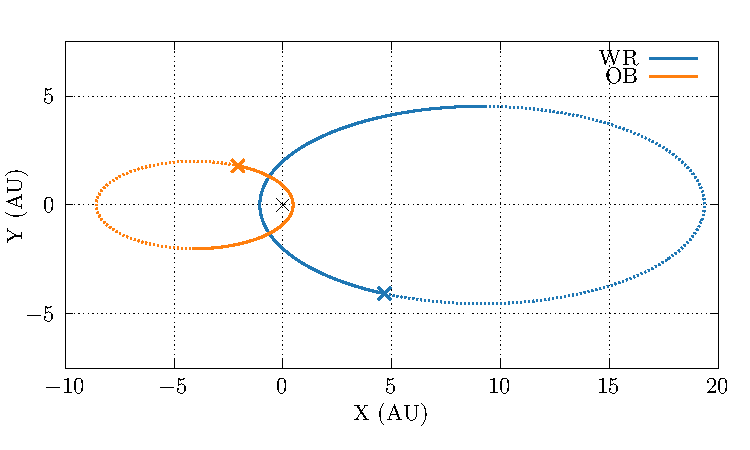
\includegraphics{assets/trajectory/wr140-orbit.pdf}
  \caption[Simulation orbital trajectories of WR140 WC7 and O5 stars]{Simulation orbital trajectories of the WC7 and O5 stars in WR140. The solid lines represent the orbital phase being simulated, corresponding to $0.95 \leq \Phi \leq 1.10$, while the dashed lines represent the full orbital trajectory. The starting position for each star and the orbital barycentre at (0,0) have been annotated.}
  \label{fig:p2-trajectory}
\end{figure}

\begin{figure}
  \centering
  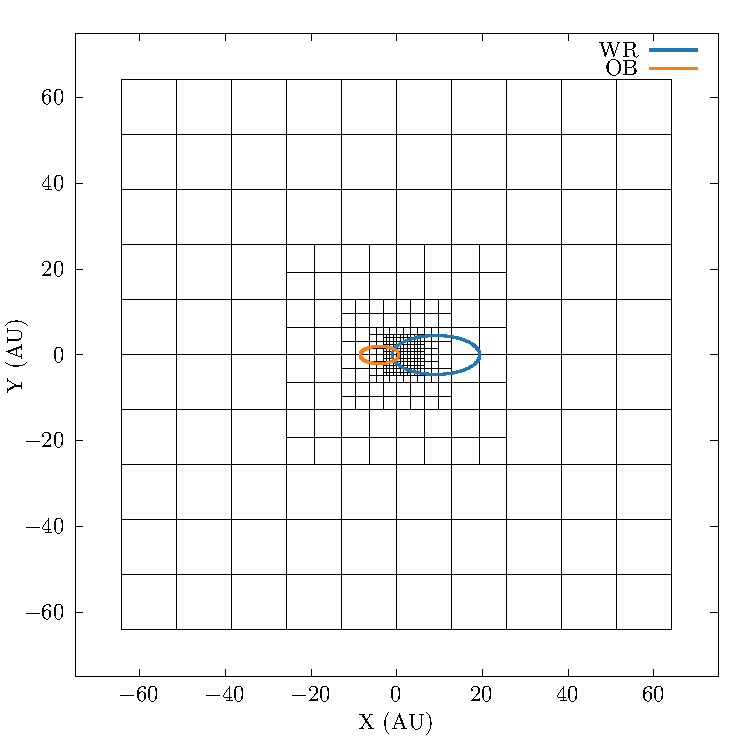
\includegraphics{assets/wr140-grid/grid-orbit.pdf}
  \caption{Numerical grid of the WR140 system simulation, static mesh refinement was used to increase the resolution around the orbital path from $0.95 \leq \Phi \leq 1.10$. The orbital path of both stars are overlaid onto this numerical grid. While the stars in the system can be within cells that are not fully refined, if there is insufficient resolution the stars begin to break down. As such the stars are typically in the 3\ts{rd} or 4\ts{th} level.}
  \label{fig:p2-orbitalpath}
\end{figure}


\subsection{Data collection}
% Data collection 
Simulation data was exported as HDF5 files at regular time intervals.
3D meshes were collected every increment of $\delta \Phi = \num{1.5e-3}$, while 2D slices in the XY plane were collected every increment of $\delta \Phi = \num{1.5e-4}$.
These HDF5 files contain the primitive variables of the simulation: gas density, $\rho$, gas pressure, $P$, and wind velocity components, $v_x$, $v_y$ and $v_z$.
These variables were then used to derive other variables such as temperature and energy.
The scalars governing the dust properties were also stored for each cell: the dust-to-gas mass ratio, $z$, and the dust grain radius, $a$.
The wind ``colour'', the proportion of gas from each star, was also stored.
A value of 1.0 indicates a pure WR wind while 0.0 indicates a pure OB wind.
The volume-weighted totals of all parameters of interest were also collected, such as the average values for $z$, $a$ and the dust production rate within the WCR, $\dot{\text{M}}\rms{d}$.
To calculate $\dot{\text{M}}\rms{d}$, a cell must be identified as being within the WCR, this was performed by comparing the cell density to the predicted density of a single wind with the wind parameters of the WC star in the system.
Any cell with a density higher a certain threshold value was flagged as being within the WCR.
the single-wind density, $\rho\rms{SW}$, was calculated using the equation:

\begin{equation}
  \rho\rms{SW} = \frac{\dot{\text{M}}\rms{SW}}{4\pi r^2 v^\infty\rms{SW}},
\end{equation}

\noindent
where $r$ is the distance from the barycentre.
This threshold value was set to $\rho\rms{thres} = 1.25\rho\rms{SW}$, which was found to accurately identify the WCR through thorough prior testing.

\section{Results and Conclusions}
\label{sec:p2-results}

% Dust production rate

\begin{table}
  \centering
  \begin{tabular}{lll}
  \hline
  Parameter & Mean & Maximum \\ \hline
  $\dot{\text{M}}\rms{d}$ (\si{\solarmass\per\year}) & \num{7.68e-08} & \num{1.24e-06} \\
  $\bar{a}$ (\si{\micro\metre}) & \num{1.32e-02} & \num{1.44e-02} \\
  $\bar{z}$ & \num{3.98e-04} & \num{3.32e-03} \\ \hline
  \end{tabular}
  \caption[Advected scalar yields from WR140 simulation]{Advected scalar yields from the WR140 simulation.}
  \label{tab:paper-2-dust-rates}
\end{table}

\begin{figure}
  \centering
  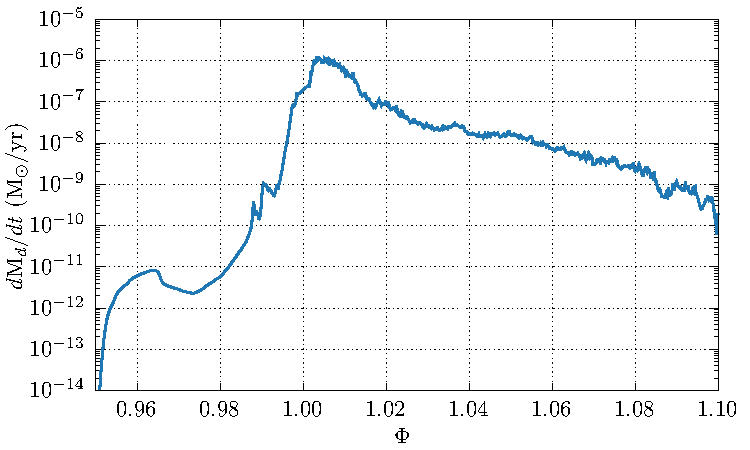
\includegraphics{assets/wr140-dust_rate.pdf}
  \caption{A graph of the dust production rate in the WCR over the orbital phase $0.95 \leq \Phi \leq 1.10$. The dust production rate sharply increases as the stars pass their closest approach. Afterwards, the dust production rate begins to falter and slow, due to weaker wind collision effects via the separation distance and radial velocity.}
  \label{fig:wr140-dustproduction}
\end{figure}

\begin{figure}
  \centering
  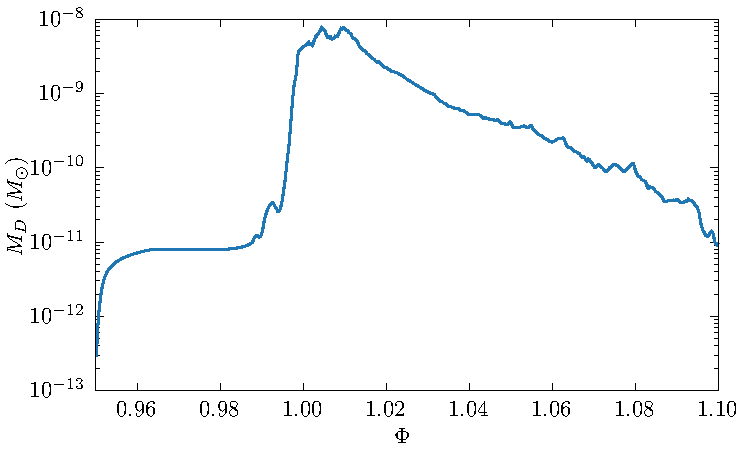
\includegraphics{assets/wr140-m_dust.pdf}
  \caption{A graph of the overall dust mass in the simulation of WR140 over the orbital phase $0.95 \leq \Phi \leq 1.10$. The amount of dust quickly reduces after periastron due to a decreased dust formation rate (Fig. \ref{fig:wr140-dustproduction}), as well as dust advecting off of the numerical grid.}
  \label{fig:wr140-dustmass}
\end{figure}

Dust production was found to be consistent with previous uses of this particular dust model.
Dust production rates were found to be sensible, and significantly below the theoretical maximum dust formation rate, $\mdot\rms{d,max} \approx \SI{4.8e-6}{\solarmass\per\year}$.
% Previous paper might be a bit of a whole thing, need to ask Julian how to reference to that
After an initial advection period lasting until $\Phi \approx 0.96$, the dust production rate rapidly increased as the stars approached periastron passage, peaking at $\Phi \sim 1.01$ (Fig. \ref{fig:wr140-dustproduction}).
This maximum dust production rate of \SI{1.24e-6}{\solarmass\per\year} is sensible, but incredibly prodigious, demonstrating a peak conversion efficiency of gas into dust of $\sim 26\%$ in the WCR and a total conversion efficiency of $\sim 2.2\%$ throughout the entire system.
After reaching this maximum value, the dust production rate steadily decreases as the stars recede from each other.
This is reflected in the overall dust mass of the simulation (Fig. \ref{fig:wr140-dustmass}), as well as in infrared observations of WR140, where the infrared emission from dust formation rapidly reaches a maximum value after periastron passage, and slowly relaxes to a minimum value. % Find citation for this, plot
This asymmetry in the time-dependent change in infrared luminosity implies the existence of several factors for suppression and encouragement of dust formation than just the change in orbital separation distance.
It should be noted that due to the small size of the simulation, the dust mass in the system will reduce quickly, as dust advects off of the numerical grid.

The evolution of dust in this system would result in the formation of an expanding cloud of dust every time the system passes periastron, with no contiguous spiral pattern forming, due to the lengthy ``dormant'' period occurring shortly after periastron passage.
This is consistent with observations of WR140, where these disconnected clouds are observed \parencite{williams_orbitally_2009}.
We find an average dust production rate of $\mdot\rms{d} = \SI{7.68e-8}{\solarmass\per\year}$, and am change in the dust production rate by approximately five orders of magnitude over the course of the simulation.
This fits our understanding of an episodic dust forming WCd system, with an extremely clear ``active'' period followed by a slow tapering off of dust production as the system approaches the ``dormant'' period.
We can compare our results to the estimated dust yields from \textcite{lauRevisitingImpactDust2020}, which found an average dust production rate of $\mdot\rms{d} = \SI{8.11e-10}{\solarmass\per\year}$.
Our value for the dust-to-gas mass ratio within the system appears to be sensible, while our average dust production rate is significantly higher.
This is due to the limited temporal sample of the simulation.
We would find a significantly lower average dust production rate over the course of a full orbit due to more sampling of the system over the ``dormant'' period.

\begin{figure}
  \centering
  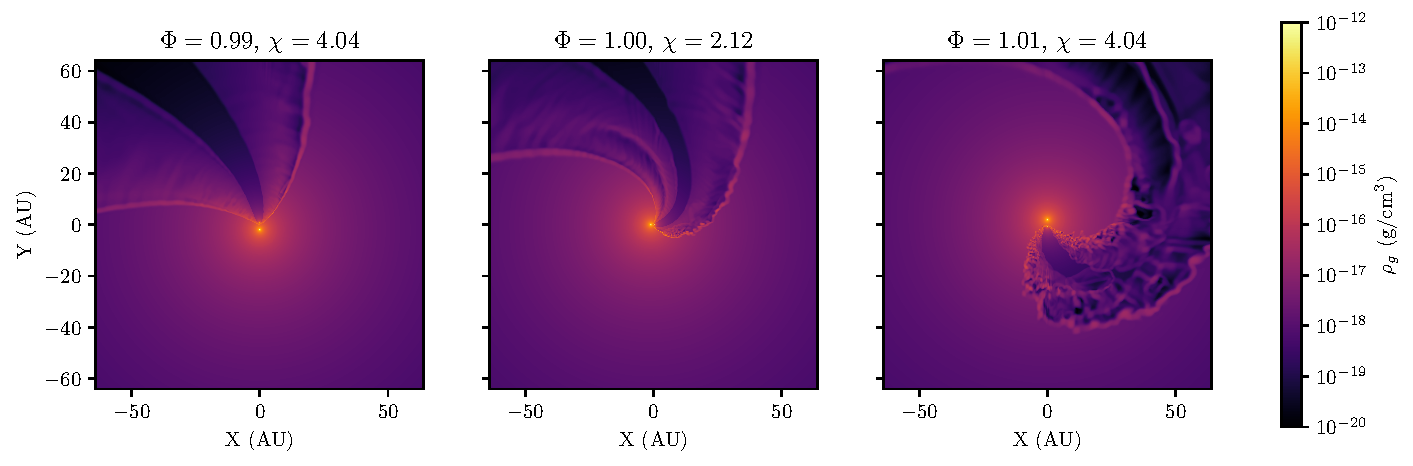
\includegraphics[width=\linewidth]{assets/periastron-3-rho.pdf}
  \caption{Gas density in a simulation of the WR140 system shortly before, during, and shortly after periastron. The simulation becomes rapidly dominated by instabilities a short while after periastron. However, these instabilities persist despite the system behaving adiabatically at a similar orbital separation distance prior to periastron. This suggests that the radiative behaviour of the post-shock WCR is due to multiple factors, other than dust a varying $d\rms{sep}$.}
  \label{fig:p2-fullpage-rho}
\end{figure}

\begin{figure}
  \centering
  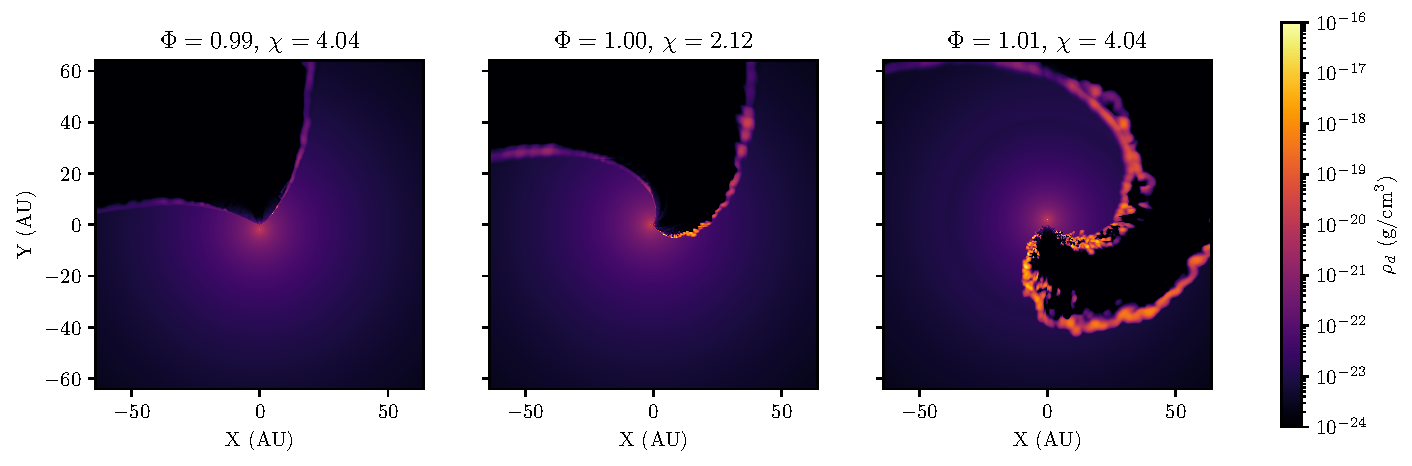
\includegraphics[width=\linewidth]{assets/periastron-3-rhod.pdf}
  \caption{Dust density in a simulation of the WR140 system shortly before, during, and shortly after periastron. Dust formation occurs as a direct result of the formation of thermal and KH instabilities in the post-shock WCR.}
  \label{fig:p2-fullpage-rhod}
\end{figure}

\begin{figure}
  \centering
  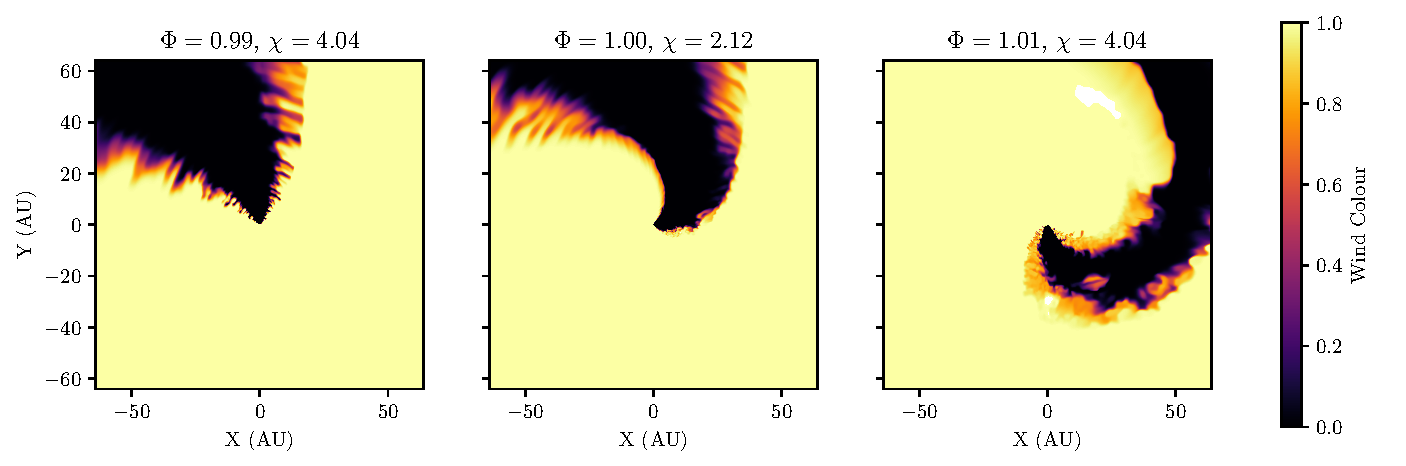
\includegraphics[width=\linewidth]{assets/periastron-3-r0.pdf}
  \caption{Wind ``colour'' in a simulation of the WR140 system shortly before, during, and shortly after periastron. With 1 representing a pure WR wind and 0 representing a pure OB wind. We find that the wind undergoes more mixing during and after periastron.}
  \label{fig:p2-fullpage-r0}
\end{figure}

\subsection{Instabilities}

% Instabilities

As can be seen in Fig. \ref{fig:p2-fullpage-rho}, after periastron passage the post-shock WCR region transitions from a smooth adiabatic wind to a highly radiative wind dominated by instabilities.
As the WCR becomes increasingly dominated by instabilities, dust formation drastically increases, with the bulk of dust formation occurring within the high density regions produced by these instabilities.
These clumpy pockets of gas do not exhibit significant dust formation beyond $\sim \SI{20}{\au}$ from the simulation barycentre, with concentrations of dust remaining approximately constant (Fig. \ref{fig:p2-fullpage-rhod}).
% Induced instabilities, ie 
By the end of the simulation at $\Phi = 1.10$, the WCR is still somewhat dominated by instabilities, with an elevated dust production rate even though the cooling parameter has increased significantly to $\chi = 19.7$, which would imply adiabatic behaviour.
Whilst the dust formation rate has reduced significantly, there is still a significantly greater formation rate than at the start of the simulation (after advection).
This suggests that the transition from radiative to adiabatic behaviour has a degree of latency, with instabilities still driving the structure of the WCR long after adiabatic flow should have been re-established.
% Wind mixing
The amount of wind being mixed in the system is also significantly increased after periastron passage, which would be conducive to the formation of complex organic molecules on the surface of the dust grains (Fig. \ref{fig:p2-fullpage-r0}).
Whilst research into this is out of the scope of the project, evolution of dust grains from WCd systems on longer time and length scales would be an enlightening avenue of research.

\subsection{Influence of varying wind velocity on dust production}

% Note change in dust yields from previous paper, will have to reference this when in publishing
As we have previously discussed, varying the wind terminal velocity for both stars in a simulation can result in exponential changes in the dust production rate.
This is theorised to be due to the increased influence of thermal instabilities through increased cooling in slower post-shock winds, as well as through KH instabilities driven through a wind velocity shear (if the wind terminal velocities are significantly different, see \cite{stevens_colliding_1992}).
Previous work on this subject considered systems with circular orbits, hence the orbital motion between the stars was persistent, and did not contribute to a change in the wind velocities over the orbit of the system.
However, in the case of a system with an eccentric orbit (such as WR140), we would find that both the outflow velocity for each wind - as well as the velocity ratio - would be markedly different over the systems orbit.
% Discuss change in relative velocity, will significantly impact, by as much as an order of magnitude? Write script to calculate change in chi?
As the stars approach periastron, the radial velocity, $v\rms{r}$ for each star rapidly changes from a minimum value to a maximum, as the stars approach and then swing past one another.
This sudden change in the stars radial velocity results in a rapid change in the velocity for both winds entering the collision region.
This will influence the amount of radiative cooling in the post-shock wind, suppressing radiative cooling pre-periastron and inciting it post-periastron, altering the dust formation rates. 
While this change in wind velocity is relatively small, with the wind velocity varying by as much as 6\% over the course of an orbit, this can still impact the cooling of the system.
Due to $\chi$ being dependent on $v^4$, this effect can vary $\chi$ by as much as a factor of 1.26 in the case of WR140.

% Velocity shear
The rate of dust formation is also strongly governed by the presence of a large wind velocity ratio, $\Upsilon$, where:

\begin{equation}
  \Upsilon = v\rms{OB} / v\rms{WR}, 
\end{equation}

\noindent
As the mass of each star is different, the change in velocity differs, causing an increased velocity ratio and therefore a stronger velocity shear.
Previous research with dust models suggests that a strong velocity shear drives an increased dust formation rate.
We find that the maximum change in velocity shear occurs at $\Phi = 1.01$, around the same time where the dust formation rate is at a maximum; this is consistent with our previous work (Fig. \ref{fig:p2-shear}).
% Whilst this will not dominate the dynamics of dust formation as a whole, this would explain asymmetry in dust formation rate curve
Whilst this change in velocity shear would not significantly alter the dynamics of dust formation on its own, it may be another factor in explaining the increased dust formation of WR140 post-periastron, and explain why the system is still dominated by instabilities even after the system should be behaving adiabatically.
However, this effect may also be decreased somewhat by the effect of radiative inhibition and braking on the winds.
We find using a model estimating wind velocities using the \textcite*{castor_radiation-driven_1975} model for radiative driving that the OB wind in particular is affected.
Fig. \ref{fig:p2-cak} shows the wind velocities resultant from this model with CAK parameters for the WR and OB stars in WR140.
We find that the wind velocity is approximately 84\% of the expected velocity.
This would decrease the velocity shear before and after periastron passage.
% reducing the velocity ratio on average, and resulting in a weaker velocity shear.
The effect of radiative line driving from the CAK model is not considered in this simulation, and simulations considering this effect would have to be performed in order to study this further.
This represents another interesting avenue of future research.



% \begin{figure}
%   \centering
%   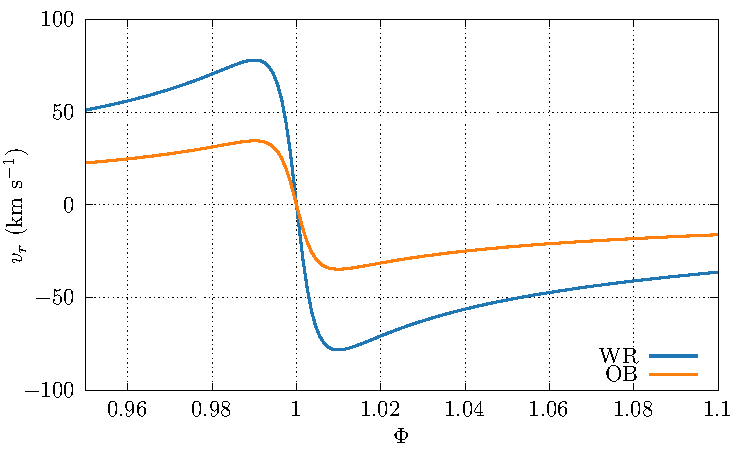
\includegraphics{assets/radial-velocity/radial.pdf}
%   \caption[Radial velocity]{Radial velocity as a function of the orbital phase for the WR and OB stars in the WR140 system relative to the barycentre. As periastron passage occurs, the sudden inversion from approaching to receding can alter the wind velocity of the WR star by as much as \SI{160}{\kilo\metre\per\second}. Whilst this discrepancy is $\sim 6\%$ of the WR wind velocity, this can significantly increase dust production if the stars are receding from each other.}
% \end{figure}

\begin{figure}
  \centering
  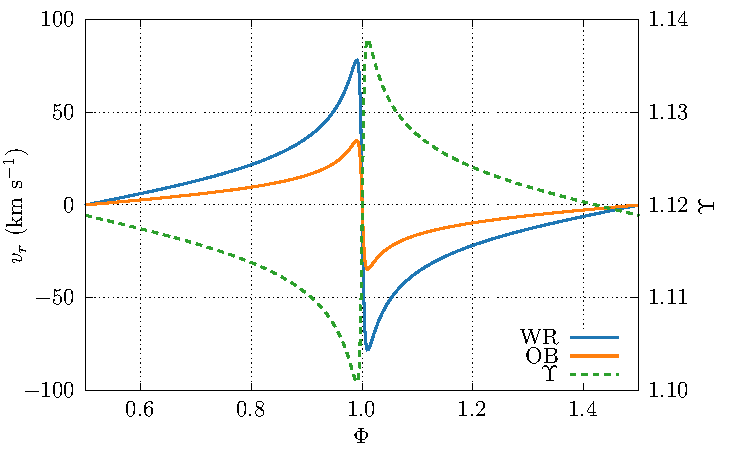
\includegraphics{assets/radial-velocity/radial-shear.pdf}
  \caption[Radial velocity]{Radial velocity as a function of the orbital phase for the WR and OB stars in the WR140 system relative to the barycentre. As periastron passage occurs, the sudden inversion from approaching to receding can alter the wind velocity of the WR star by as much as \SI{160}{\kilo\metre\per\second}. Whilst this discrepancy is $\sim 6\%$ of the WR wind velocity, this can significantly increase dust production if the stars are receding from each other. The velocity shear, $v\rms{OB}/v\rms{WR}$, also sharply increases during periastron passage, peaking at the point of maximum dust formation.}
  \label{fig:p2-shear}
\end{figure}

\begin{figure}
  \centering
  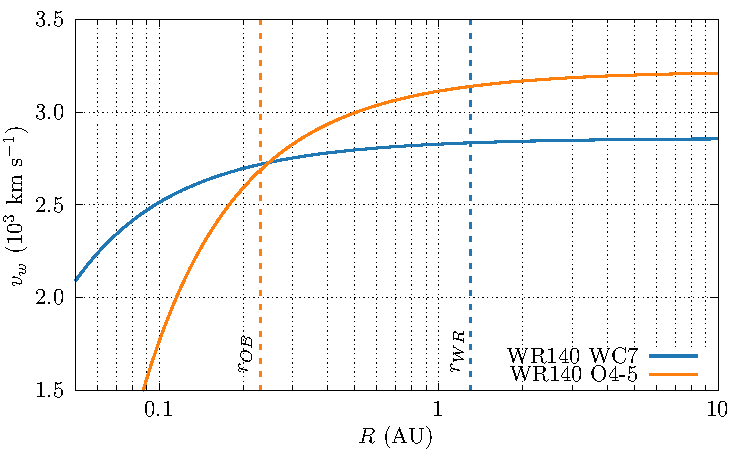
\includegraphics{assets/stag.pdf}
  \caption{Graph of the wind velocity of the WC7 and O4-5 stars in the WR140 system as a function of distance from the stellar surface due to radiative line driving. The dashed lines represent the distance to the WCR at periastron for each star. During periastron passage the WC7 wind is travelling at approximately its terminal velocity before collision, while the O4-5 companions wind is travelling at $\sim 84\%$ of terminal velocity before coming into contact with the WCR. CAK parameters were estimated to be $k = 0.37$, $\alpha = 0.60$ for the O4-5 star and $k=0.48$, $\alpha = 0.57$ for the WC7 star.}
  \label{fig:p2-cak}
\end{figure}


\section{Summary}
\label{sec:p2-conclusion}

Despite only simulating a limited section of the orbit of WR140, we have made a number of insights into the behaviour of the system.
We find a significant degree of change in the dust formation rate as a direct consequence of the changing orbital separation of the system.
This is related to the change in the behaviour of the post-shock WCR wind, which goes from a smooth adiabatic wind to a clumpy, high density wind dominated by instabilities ideal for dust formation.
It is particularly interesting to note that the system does not revert to behaving adiabatically as quickly as it entered it.
This suggests that the post-shock WCR condition of the system is dependent on additional factors, instead of being solely due to $d\rms{sep}$.
One of the main factors on this delayed return to the adiabatic, ``dormant'' state is potentially due to the orbital motion of the stars themselves.
As the stars approach each other at periastron, the radial velocity of the stars adds velocity to the wind beyond the outflow velocity, resulting in higher wind collision velocities, which encourages adiabatic behaviour in the post-shock flow.
The inverse is true as the stars recede from one another, the effective wind velocity for both stars is reduced, which encourages the formation of thermal instabilities.
Furthermore, as the OB star dominates the orbital dynamics of the system, the effective WR wind velocity is even further reduced, leading to an increased wind velocity ratio, resulting in a velocity shear that can drive KH instabilities.

There is much additional research potential in simulating dust growth in episodic WCd systems.
Further simulations of this system in particular would involve simulating a full orbit, through the use of AMR and increased computing time.
Other avenues of research include the effect on dust formation due to the influence of radiative line driving and sudden braking, as well as a more complex, multi-fluid dust model where dust grains are not explicitly coupled to the stellar wind.

\section{Acknowledgements}

This work was undertaken on ARC4, part of the High Performance Computing facilities at the University of Leeds, UK.
We would also like to thank P. A. Crowther for his work on the \footlink{Galactic Wolf-Rayet Catalogue}{pacrowther.staff.shef.ac.uk/WRcat}.
\chapter[Influence of Wind Velocity on Dust Formation]{An Exploration on the Influence of Wind Velocity of Dust formation in WCd Systems}

\section{Introduction}

\section{Methodology}

\section{Model Parameters}

\begin{table}[]
  \centering
  \begin{tabular}{cccccc}
  \hline
  Model & $v^\infty_{WR}$ & $v^\infty_{OB}$ & $\eta$ & $\chi_{WR}$ & $\chi_{OB}$ \\
   & \si{\centi\metre\per\second} & \si{\centi\metre\per\second} &  &  &  \\ \hline
  \texttt{sim-1-wr} & \num{2.00e+08} & \num{2.00e+08} & 0.010 & 19.149 & 1915 \\
  \texttt{sim-2-wr} & \num{1.36e+08} & \num{2.00e+08} & 0.015 & 4.060 & 1915 \\
  \texttt{sim-3-wr} & \num{1.03e+08} & \num{2.00e+08} & 0.019 & 1.332 & 1915 \\
  \texttt{sim-4-wr} & \num{8.26e+07} & \num{2.00e+08} & 0.024 & 0.557 & 1915 \\
  \texttt{sim-5-wr} & \num{6.91e+07} & \num{2.00e+08} & 0.029 & 0.273 & 1915 \\
  \texttt{sim-6-wr} & \num{5.94e+07} & \num{2.00e+08} & 0.034 & 0.149 & 1915 \\
  \texttt{sim-7-wr} & \num{5.21e+07} & \num{2.00e+08} & 0.038 & 0.088 & 1915 \\
  \texttt{sim-8-wr} & \num{4.63e+07} & \num{2.00e+08} & 0.043 & 0.055 & 1915 \\
  \texttt{sim-9-wr} & \num{4.18e+07} & \num{2.00e+08} & 0.048 & 0.036 & 1915 \\
  \texttt{sim-10-wr} & \num{3.80e+07} & \num{2.00e+08} & 0.053 & 0.025 & 1915 \\
  \texttt{sim-11-wr} & \num{3.49e+07} & \num{2.00e+08} & 0.057 & 0.018 & 1915 \\
  \texttt{sim-12-wr} & \num{3.22e+07} & \num{2.00e+08} & 0.062 & 0.013 & 1915 \\
  \texttt{sim-13-wr} & \num{2.99e+07} & \num{2.00e+08} & 0.067 & 0.010 & 1915 \\
  \texttt{sim-14-wr} & \num{2.79e+07} & \num{2.00e+08} & 0.072 & 0.007 & 1915 \\
  \texttt{sim-15-wr} & \num{2.62e+07} & \num{2.00e+08} & 0.076 & 0.006 & 1915 \\
  \texttt{sim-16-wr} & \num{2.47e+07} & \num{2.00e+08} & 0.081 & 0.004 & 1915 \\
  \texttt{sim-17-wr} & \num{2.33e+07} & \num{2.00e+08} & 0.086 & 0.004 & 1915 \\
  \texttt{sim-18-wr} & \num{2.21e+07} & \num{2.00e+08} & 0.091 & 0.003 & 1915 \\
  \texttt{sim-19-wr} & \num{2.10e+07} & \num{2.00e+08} & 0.095 & 0.002 & 1915 \\
  \texttt{sim-20-wr} & \num{2.00e+07} & \num{2.00e+08} & 0.100 & 0.002 & 1915 \\ \hline
  \end{tabular}
  \caption{WR parameters}
  \label{tab:vinf-chi-wrparams}
\end{table}

\begin{table}[]
  \centering
  \begin{tabular}{cccccc}
  \hline
  Model & $v^\infty_{WR}$ & $v^\infty_{OB}$ & $\eta$ & $\chi_{WR}$ & $\chi_{OB}$ \\
   & \si{\centi\metre\per\second} & \si{\centi\metre\per\second} &  &  &  \\ \hline
  \texttt{sim-1-ob} & \num{1.00e+08} & \num{1.00e+08} & 0.010 & 1.197 & 120 \\
  \texttt{sim-2-ob} & \num{1.00e+08} & \num{1.47e+08} & 0.015 & 1.197 & 564 \\
  \texttt{sim-3-ob} & \num{1.00e+08} & \num{1.95e+08} & 0.019 & 1.197 & 1721 \\
  \texttt{sim-4-ob} & \num{1.00e+08} & \num{2.42e+08} & 0.024 & 1.197 & 4112 \\
  \texttt{sim-5-ob} & \num{1.00e+08} & \num{2.89e+08} & 0.029 & 1.197 & 8403 \\
  \texttt{sim-6-ob} & \num{1.00e+08} & \num{3.37e+08} & 0.034 & 1.197 & 15407 \\
  \texttt{sim-7-ob} & \num{1.00e+08} & \num{3.84e+08} & 0.038 & 1.197 & 26079 \\
  \texttt{sim-8-ob} & \num{1.00e+08} & \num{4.32e+08} & 0.043 & 1.197 & 41520 \\
  \texttt{sim-9-ob} & \num{1.00e+08} & \num{4.79e+08} & 0.048 & 1.197 & 62975 \\
  \texttt{sim-10-ob} & \num{1.00e+08} & \num{5.26e+08} & 0.053 & 1.197 & 91833 \\
  \texttt{sim-11-ob} & \num{1.00e+08} & \num{5.74e+08} & 0.057 & 1.197 & 129630 \\
  \texttt{sim-12-ob} & \num{1.00e+08} & \num{6.21e+08} & 0.062 & 1.197 & 178045 \\
  \texttt{sim-13-ob} & \num{1.00e+08} & \num{6.68e+08} & 0.067 & 1.197 & 238900 \\
  \texttt{sim-14-ob} & \num{1.00e+08} & \num{7.16e+08} & 0.072 & 1.197 & 314164 \\
  \texttt{sim-15-ob} & \num{1.00e+08} & \num{7.63e+08} & 0.076 & 1.197 & 405950 \\
  \texttt{sim-16-ob} & \num{1.00e+08} & \num{8.11e+08} & 0.081 & 1.197 & 516516 \\
  \texttt{sim-17-ob} & \num{1.00e+08} & \num{8.58e+08} & 0.086 & 1.197 & 648263 \\
  \texttt{sim-18-ob} & \num{1.00e+08} & \num{9.05e+08} & 0.091 & 1.197 & 803739 \\
  \texttt{sim-19-ob} & \num{1.00e+08} & \num{9.53e+08} & 0.095 & 1.197 & 985633 \\
  \texttt{sim-20-ob} & \num{1.00e+08} & \num{1.00e+09} & 0.100 & 1.197 & 1196783 \\ \hline
  \end{tabular}
  \caption{OB parameters}
  \label{tab:vinf-chi-obparams}
\end{table}

\section{Results}
\chapter{Final Notes and Conclusions}

\section{Conclusions}

\subsection{Causes of dust formation in WCB systems}

\subsection{The role of eccentricity in dust formation}

\section{Future Study}

\subsection{More complex models}

\subsection{Further simulations of observed systems}

\subsection{Radiative transfer}

\subsection{WR+WR systems}

\subsection{Next generation telescopes}

\section{Other Observations}

\subsection[\textit{How I Learned to Stop Worrying and Love Numerics}]{\textit{Doctorate Strangelove or: How I Learned to Stop Worrying and Love Numerics}} 

\subsection{Join the physics department, see the world}

\subsection{Paul Erd\H{o}s was probably onto something}

\subsection{Carinae Strain: PhD research in a time of pandemic}

\subsection{WR 104 as a local GRB candidate}




%\appendix
\appendix
% Each appendix section has its own individual folder, containing a tex file and figures folder
\chapter{Astrophysical Shocks}

% References separate from main matter or appendix
\addcontentsline{toc}{chapter}{References} % Adds References to contents page
\printbibheading
\printbibliography[type=book,notkeyword=software,heading=subbibliography,title={Book Citations}]
\printbibliography[type=article,notkeyword=software,heading=subbibliography,title={Journal Citations}]
\printbibliography[keyword=software,heading=subbibliography,title={Software Citations}]
\printbibliography[nottype=book,nottype=article,notkeyword=software,heading=subbibliography,title={Other Citations}]

\end{document}
